%! TeX root = /Users/trustinnguyen/Downloads/Berkeley/Math/Math104/Notes/Math104Notes.tex

\documentclass{report}
\usepackage{/Users/trustinnguyen/.mystyle/math/packages/mypackages}
\usepackage{/Users/trustinnguyen/.mystyle/math/commands/mycommands}
\usepackage{/Users/trustinnguyen/.mystyle/math/environments/report}
\graphicspath{{./figures/}}

\title{Math104Notes}
\author{Trustin Nguyen}

\begin{document}
\newgeometry{
    total={150mm,235mm},
}

\begin{titlepage}
    \maketitle
\end{titlepage}
\tableofcontents
\restoregeometry

\reversemarginpar

\chapter{Week 1}

\textbf{Notations}: For sets, we have a set $S$ is a collection of elements. Either $x \in S$ or $x \notin S $. If $S^{\prime} \subseteq S$ if $S^{\prime}$ has elements that all are in $S$. Intersection and union:
    \begin{align*}
        S_{1} \cap S_{2} = \{s : s \in S_{1} \text{ and } s \in S_{2}\} \\
        S_{1} \cup  S_{2} = \{s : s \in S_{1} \text{ or } s \in S_{2}\} \\
        S_{1} - S_{2} = \{s : s \in S_{1} \text{ and } s \notin S_{2}\}
    \end{align*}
We also have other common types of sets:
    \begin{align*}
        \mathbb{N} &= \{1, 2, 3, \ldots\}                                          \\
        \mathbb{Z} &= \{\ldots, -1, 0, 1, \ldots\}                                 \\
        \mathbb{Q} &= \{\dfrac{p}{q} : p, q \in \mathbb{Z} \text{ and } q \neq 0\} \\
        \mathbb{R} &= \text{Real numbers}                                            
    \end{align*}

\begin{topic}
    \section{Absolute Values (Ross 3)}
\end{topic}

\begin{definition}{Absolute Values}
        $\forall a \in \mathbb{R}$:
            \begin{equation*}
                \lvert a \rvert = 
                    \begin{cases}
                        a \text{ if } a \geq 0 \\
                        a \text{ if } a < 0
                    \end{cases}
            \end{equation*}
        You could also say that the absolute value is the distance between $a$ and $0$.
    \end{definition}

\begin{theorem}{Absolute values}
    The following are facts about absolute values:
    \begin{itemize}
        \item $\lvert a \rvert \geq 0$
            \begin{proof}
                We follow by the function of the definition of absolute values. Use case work.
            \end{proof}

        \item $\lvert ab \rvert = \lvert a \rvert\lvert b \rvert$
            \begin{proof}
                
            \end{proof}

        \item $\lvert a + b \rvert \leq \lvert a \rvert + \lvert b \rvert$
            \begin{proof}
                For two numbers we have:
                    \begin{align*}
                        -\lvert a \rvert &\leq  a \leq \lvert a \rvert \\
                        -\lvert b \rvert &\leq  b \leq \lvert b \rvert   
                    \end{align*}
                We have that 
                    \begin{equation*}
                        -(\lvert a \rvert + \lvert b \rvert) \leq a + b \leq \lvert a \rvert + \lvert b \rvert
                    \end{equation*}
                We then have
                    \begin{align*}
                        a + b    &\leq \lvert a \rvert + \lvert b \rvert \\
                        -(a + b) &\leq \lvert a \rvert + \lvert b \rvert   
                    \end{align*}
                By case work, $\lvert a + b \rvert \leq \lvert a \rvert + \lvert b \rvert$. This is called the triangle inequality because it says that the sum of two sides of a triangle is greater than or equal to the third.
            \end{proof}
    \end{itemize}
\end{theorem}

\begin{examples}
    \begin{example}
        Show that $\sqrt{2}$ is irrational.
            \begin{proof}
                Suppose for contradiction that $\sqrt{2}$ is a rational number. So we have $p, q$ which are integers such that:
                    \begin{equation*}
                        \sqrt{2} = \frac{p}{q}
                    \end{equation*}
                where $q \neq 0$ and $p, q$ are relatively prime. 
                    \begin{align*}
                        \frac{p}{q}         &= \sqrt{2} \\
                        \frac{p^{2}}{q^{2}} &= 2        \\
                        p^{2}               &= 2q^{2}     
                    \end{align*}
                So $p^{2}$ must be even. So there exists an $m$ such that $p = 2m$. Now we have
                    \begin{align*}
                        (2m)^{2} &= 2q^{2} \\
                        4m^{2}   &= 2q^{2} \\
                        2m^{2}   &= q^{2}    
                    \end{align*}
                This also means that $q^{2}$ is even. But that is a contradiction as $p, q$ are relatively prime.
            \end{proof}
    \end{example}
\end{examples}

\begin{topic}
    \section{Lower and Upper Bounds/ Completeness Axiom}
\end{topic}

\begin{definition}{Maximum/Minimum of $S \subseteq \mathbb{R}$}
    If $\exists x_{0} \in S$ such that $\forall x \in S$, $x_{0} \geq  x$, we call $x_{0}$ the maximum of $S$. $x_{0} = \max(S) $

    If $\exists x_{0} \in S$ such that $x_{0} \leq x$ for all $x \in S$, then $x_{0}$ is the minimum of $S$.
\end{definition}

The maximum or minimum may not exist. It is unique if it exists also.

\begin{examples}
    \begin{example}
        We have the set $\{1, 2, 3, 4\}$. The max is $4$ and the min is $1$
    \end{example}

    \begin{example}
        We have the set $(0, 10) = \{x \in \mathbb{R}: x > 0 \land x <  10\}$. There is no maximum nor minimum.
    \end{example}

    \begin{example}
        We have the set $[0, \infty) = \{ x \in \mathbb{R}: x \geq 0\}$. The maximum does not exist. The minimum is $0$.
    \end{example}
\end{examples}

\begin{definition}{Upper/Lower Bound}
    If $\exists M \in \mathbb{R}$ where $\forall x \in S$, $M \geq x$, then $M$ is the upper bound of a set $S$. Note that unlike the maximum, $M$ does not have to be in $S$. 

    If $\exists m \in \mathbb{R}$ where $\forall x \in S$, $m \leq x$, then $m$ is the lower bound of $S$.

    We say that $S$ is bounded above if the upper bound exists. If $S$ has a lower bound, we say that $S$ is bounded below. If $S$ is bounded above and below, $S$ is said to be bounded.
\end{definition}

\begin{examples}
    \begin{example}
        $S = (0, 1) = \{x \in \mathbb{R} : 0 <  x <  1\}$. We have the upper bound as $M \geq 1$. The lower bound is $m \leq 0$.
    \end{example}

    \begin{example}
        $S = (-\infty, 1]$. The upper bound is $M \geq 1$. There is no lower bound.
    \end{example}
\end{examples}

Remark: The upper and lower bound may not exist. They also need not be unique. If the maximum of $S$ exists, then the maximum is an upper bound. The same can be said for the minimum of $S$.

\begin{definition}{Sup/Inf}
    If $\exists x_{0} \in \mathbb{R}$ such that:
        \begin{itemize}
            \item $x_{0}$ is an upper bound of $S$.

            \item $x_{0}$ is the smallest upper bound,
        \end{itemize}
    then we say that $x_{0}$ is the supremum of $S$. $\text{Sup}(S) = x_{0}$.

    If $\exists x_{0}^{\prime} \in \mathbb{R}$ such that:
        \begin{itemize}
            \item $x_{0}^{\prime}$ is a lower bound of $S$

            \item $x_{0}^{\prime}$ is the largest lower bound of $S$,
        \end{itemize}
    then we call $x_{0}$ the infimum of $S$ or $\text{Inf}(S) = x_{0}^{\prime}$.

    Note that the infimum and supremum may not exist but if they do, they are unique.
\end{definition}

If $\max(S)$ exists, then it is equal to $\sup (S)$. If $\sup (S)$ exists, then $\max(S)$ may not exist.

\begin{examples}
    \begin{example}
        $S = (0, 2)$. We have $\inf (S) = 0$ and $\sup (S) = 2$. Notice that the maximum and minimum does not exist.
    \end{example}

    \begin{example}
        $S = \{x : x^{2} <  2\}$. This is just $(-\sqrt{2}, \sqrt{2})$. This goes back to the previous example.
    \end{example}
\end{examples}

Question: Can we always find a smallest upper bound if an upper bound exists?

Completeness Axiom: If $S$ is bounded above, then $\sup (S)$ exists. Corollary: If $S$ is bounded below, then $\inf (S)$ will exist. 

\begin{examples}
    \begin{example}
        Consider the set $A = \{x \in \mathbb{Q}: x \geq 0 \land x^{2} \leq  2\} = (o, \sqrt{2}) \cap \mathbb{Q}$. $A$ is bounded, but $A$ has no supremum in $\mathbb{Q}$.
    \end{example}
\end{examples}

\begin{theorem}{Archimedian Property}
    If $a, b > 0$, then $\exists n \in \mathbb{N}$, we have $na > b$.
\end{theorem}
\begin{proof}
    Assume for any $a$, $na \leq b$ for all $n \in \mathbb{N}$. Let $S = \{na : n \in \mathbb{N}\}$. Then $S$ is bounded above. So $\sup (S) - a$ is not an upper bound of $S$. So $\exists n_{0} \in \mathbb{N}$ such that $na > \sup (S) - a$: $(n_{0} + 1)a >  \sup (S)$. But $n_{0} + 1 \in \mathbb{N}$, so it must be in $S$. This is a contradiction.
\end{proof}

\begin{theorem}{$\mathbb{Q}$ is dense}
    If $a, b \in \mathbb{R}$ and $a < b$, then there exists $r \in \mathbb{Q}$ such that $a < r < b$.
\end{theorem}

The idea is that we want to find $\frac{m}{n}$ that is between $a$ and $b$. This is equivalent to $an < m < bn$. We want $n$ such that $nb - na >  1$. But this is just the archimedian property: $n(a - b) > 1$

\chapter{Week 2}

We will prove the denseness of the rationals using the archimedian property:
    \begin{proof}
        Let $a, b$ be in $\mathbb{R}$. Choose a $k \in \mathbb{N}$ such that $\lvert nb \rvert, \lvert na \rvert <  k$. Consider the set of $\{n \in \mathbb{Z} : na <  j < k\}$. This set is finite, so we can find the minimum of this set. We have that $m - 1 \leq na$ which means that $m \leq na + 1 < nb$. So $na < m < nb$.
    \end{proof}

\begin{topic}
    \section{Sequence and Convergence}
\end{topic}

\begin{definition}{Sequence}
    A sequence is a function from $\{n \in \mathbb{Z}: n \geq m\}$ where we usually choose $m = 0, 1$. The value is $S(n) \in \mathbb{R}$. We write the sequence  $(S_{n})_{n = m}^{\infty}$. If $m = 1$, we just write $(S_{n})$.
\end{definition}

Remark: Sometimes, we use notations $(a_{n}), (b_{n}), (C_{n})$

\begin{examples}
    \begin{example}
        We can have $S_{n} = \frac{1}{n^{2}}, n \in \mathbb{N}$ which is the sequence:
            \begin{equation*}
                (1, \dfrac{1}{4}, \dfrac{1}{9}, \dfrac{1}{16}, \ldots)
            \end{equation*}
    \end{example}
    \begin{example}
        $a_{n} = (-1)^{n}$ where $n \in \mathbb{Z}_{\geq 0}$ which is the sequence:
            \begin{equation*}
                (1, -1, 1, -1, \ldots)
            \end{equation*}
    \end{example}
    \begin{example}
        \begin{itemize}
            \item $a_{n} = \cos{\frac{n\pi}{3}}, n \in \mathbb{N}$.

            \item $a_{1} = \cos{\frac{\pi}{3}} = \frac{1}{2}$

            \item $a_{2} = \cos{\frac{2\pi}{3}} = \frac{-1}{2}$

            \item $a_{3} = \cos{\pi} = -1$

            \item $(\frac{1}{2}, -\frac{1}{2}, -1, \ldots)$ 
        \end{itemize}
    \end{example}
    \begin{example}
        $a_{n} = \sqrt[n]{n}, n \in \mathbb{N}$ with the sequence:
            \begin{equation*}
                (1, \sqrt{2}, \sqrt[3]{3}, \ldots)
            \end{equation*}
    \end{example}
\end{examples}

We will now consider limits of a sequence:
\begin{definition}{Limits of a Sequence}
    Consider $(S_{n})_{n \in \mathbb{N}} \text{ or } (S_{n})$ is said to converge to some real number $s \in \mathbb{R}$ provided that $\forall \varepsilon \geq 0, \exists N \in \mathbb{N}$ such that $\forall n >  N$, we have $\lvert S_{n} - S \rvert <  \mathcal{E}$.
\end{definition}

Remark: We usually use $\varepsilon$ for very small positive numbers.
    \begin{itemize}
        \item Choice of $N$ depended on our choice of $\varepsilon$.
    \end{itemize}

Today, we will cover rigorous proofs on convergence. 

\textbf{Proposition}: If $(S_{n})$ has limits, then the limits are unique. 
    \begin{proof}
        Assume $\lim S_{n} = S$, and that $\lim S_{n} = T$. By definition $\forall \mathcal{E} > 0, \exists N_{1}$ such that $\forall n > N$, 
            \begin{equation*}
                \lvert S_{n} - S \rvert < \mathcal{E}
            \end{equation*}
        But we have a second limit so $\exists N_{2}$ such that $\forall n > N_{2}$:
            \begin{equation*}
                \lvert S_{n} - T \rvert < \mathcal{E}
            \end{equation*}
        Recall that $\lvert a + b \rvert \leq \lvert a \rvert + \lvert b \rvert$. Take $a = S_{n} - S, b = T - S_{n}$. Then $a + b = T - S$ and 
            \begin{align*}
                \lvert a + b \rvert = \lvert T - S \rvert &\leq \lvert S_{n} - S \rvert + \lvert T - S_{n} \rvert \\
                &< 2\mathcal{E}
            \end{align*}
        So $\lvert T - S \rvert = 0$. So $T = S$.
    \end{proof}

How to prove $\lim (S_{n}) = S$ when $S_{n}$ is a function of $n$. So for $\forall \mathcal{E} >  0$, we find $N$ such that $\forall n > N$, we have $\lvert S_{n} - S \rvert <  \mathcal{E}$. So we reduce $\lvert S_{n} - S \rvert <  \mathcal{E}$ to the inequality $n > $?.

\begin{examples}
    \begin{example}
        Prove that $\lim (\frac{1}{n^{2}}) = 0$
            \begin{proof}
                $\forall \mathcal{E} > 0$, we want to find $N$ such that $\forall n > N$, $\lvert \frac{1}{n^{2}} - 0 \rvert = \frac{1}{n^{2}} <  \mathcal{E}$. So we get:
                    \begin{equation*}
                        n >  \frac{1}{\sqrt{\mathcal{E}}}
                    \end{equation*}
                So we choose $N = \frac{1}{\sqrt{\mathcal{E}}}$. So 
                    \begin{equation*}
                        \lvert \frac{1}{n^{2}} \rvert = \frac{1}{n^{2}}
                    \end{equation*}
                and since $n >  \frac{1}{\sqrt{\varepsilon}}$, $\frac{1}{n^{2}} <  \frac{1}{(\frac{1}{\sqrt{\varepsilon}})^{2}} = \varepsilon$. Then $\lim (\frac{1}{n^{2}}) = 0$
            \end{proof}
    \end{example}
    \begin{example}
        Prove $\lim (\frac{3n + 1}{7n - 4}) = \frac{3}{7}$. Idea to find the limit:
            \begin{equation*}
                \dfrac{3n + 1}{7n - 4} = \dfrac{3 + \frac{1}{n}}{7 - \frac{4}{n}} = \frac{3}{7}
            \end{equation*}
        \begin{proof}
            $\forall \varepsilon> 0$, we want to find $N$ such that $\forall n > N$, we have $\lvert \frac{3n + 1}{7n - 4} - \frac{3}{7} \rvert <  \varepsilon$
                \begin{equation*}
                    \dfrac{3n + 1}{7n - 4} - \frac{3}{7} = \dfrac{7(3n + 1) - 3(7n - 4)}{(7n - 4)7} = \dfrac{19}{7(7n - 4)}
                \end{equation*}
            So we want to find $N$ such that:
                \begin{equation*}
                    \lvert \dfrac{19}{7(7n - 4)} \rvert <  \varepsilon 
                \end{equation*}
            or
                \begin{equation*}
                    \varepsilon < \dfrac{19}{7(7n - 4)} <  \varepsilon 
                \end{equation*}
            Since $7n - 4 > 0$, $\dfrac{19}{7(7n - 4)} > 0$. Solve:
                \begin{equation*}
                    \dfrac{19}{7(7n - 4)} < \varepsilon \implies n > \dfrac{19}{49\varepsilon} + \dfrac{4}{7}
                \end{equation*}
            So now we take $N = \frac{19}{49\varepsilon} + \frac{4}{7}$. Then verify.
        \end{proof}
    \end{example}
    \begin{example}
        Prove that $\frac{4n^{3}  + 3n}{n^{3} - 6} = 4$. 
            \begin{proof}
                $\forall \varepsilon > 0$, find $N$ such that $\forall n> N$, we have:
                    \begin{equation*}
                        \lvert \dfrac{4n^{3} + 3n}{n^{3} - 6}  - 4 \rvert < \varepsilon
                    \end{equation*}
                We have:
                    \begin{equation*}
                        \dfrac{4n^{3} + 3n}{n^{3} - 6} - 4 = \dfrac{3n  + 24}{n^{3} - 6}
                    \end{equation*}
                When $n \geq 2$, $n^{3} - 6 > 0$, $\frac{3n + 24}{n^{3} - 6} > 0$. We want to find function $f$ such that:
                    \begin{equation*}
                        \dfrac{3n + 24}{n^{3} - 6} < f
                    \end{equation*}
                and $f < \varepsilon$. Since $3n + 24 \leq 27n$ and $n^{3} - 6 \geq \frac{1}{2}n^{3}$. When $n \geq 3$. So when $n \geq 3$, $\frac{3n + 24}{n^{3} - 6} \leq \dfrac{27n}{\frac{1}{2}n^{3}} = \frac{54}{n^{2}}$. So for $\frac{54}{n^{2}} <  \varepsilon$, we need: $n>  \sqrt{\frac{54}{\varepsilon}}$. So we need $n > \max(3, \sqrt{\frac{54}{\varepsilon}})$
            \end{proof}
    \end{example}
\end{examples}

\begin{topic}
    \section{Divergence}
\end{topic}

\begin{examples}
    \begin{example}
        Prove $a_{n} = (-1)^{n}$ diverges. Idea assume $\lim a_{n} = a$. We know that
            \begin{equation*}
                \text{dist}(-1, a) + \text{dist}(1, a) \geq \text{dist}(-1, 1) = 2
            \end{equation*}
        One of $\text{dist}(-1, a)$ or $\text{dist}(1, a)$ must be greater than or equal to $1$.
            \begin{proof}
                Assume $\lim (a_{n}) = a$. Let $\varepsilon = 1$. By definition, there is an $N$ such that for all $n > N$, 
                    \begin{equation*}
                        \lvert (-1)^{n} - a \rvert < 1
                    \end{equation*}
                We choose an odd and an even $n > N$ so
                    \begin{equation*}
                        \lvert 1 - a \rvert < 1 \hspace{30pt}  \text{and} \hspace{30pt} \lvert -1 - a \rvert  < 1
                    \end{equation*}
                By triangle inequality:
                    \begin{equation*}
                        \lvert 1 - a \rvert + \lvert a + 1 \rvert \geq \lvert 2 \rvert = 2
                    \end{equation*}
                But their sum should be less than $2$. So that is a contradiction.
            \end{proof}
    \end{example}
    \begin{example}
        Assume $s_{n} > 0$ and $\lim s_{n} = s> 0$. Prove 
            \begin{equation*}
                \lim \sqrt{s_{n}} = \sqrt{s}.
            \end{equation*}
        Idea: For $\forall \varepsilon > 0$, we want to find $N$ such that $\forall n > N$, $\lvert \sqrt{s_{n}} - \sqrt{s} \rvert < \varepsilon$. Recall that $(a + b) (a - b) = a^{2} - b^{2}$. So $a - b = \frac{a^{2} - b^{2}}{a + b}$. We have
            \begin{align*}
                \lvert \sqrt{s_{n}} - \sqrt{s} \rvert &= \lvert \dfrac{s_{n} - s}{\sqrt{s_{n}} + s} \rvert \\
            \end{align*}
        Since $\sqrt{s_{n}} + \sqrt{s} > \sqrt{s}$, we have
            \begin{align*}
                \dfrac{s_{n} - s}{\sqrt{s_{n}} + \sqrt{s}} &=  \dfrac{\lvert s_{n} - s \rvert}{\sqrt{s_{n}} + \sqrt{s}} \\
                                                           &<  \dfrac{\lvert s_{n} - s \rvert}{\sqrt{s}}                  
            \end{align*}
        So we solve for $\varepsilon$:
            \begin{align*}
                \dfrac{\lvert s_{n} - s \rvert}{\sqrt{s}} < \varepsilon &\iff  \lvert s_{n} - s \rvert < \varepsilon\sqrt{s} = \varepsilon   
            \end{align*}
        \begin{proof}
            We need to show that $\forall \varepsilon > 0$, we choose $\varepsilon = \varepsilon\sqrt{s}$. For $\varepsilon^{\prime}$, there is an $N$ such that $\forall n > N$, $\lvert S_{n} - s \rvert < \varepsilon^{\prime} = \varepsilon\sqrt{s}$. We have
                \begin{equation*}
                    \lvert \sqrt{s_{n}} - \sqrt{s} \rvert = {s_{n} - s}{\sqrt{s_{n}} + \sqrt{s}} < \dfrac{\lvert s_{n} - s \rvert}{\sqrt{s}} < \frac{\varepsilon\sqrt{s}}{\sqrt{s}} = \varepsilon
                \end{equation*}
            Why can't we choose $\varepsilon = (\sqrt{s_{n}} + \sqrt{s}) \varepsilon$? Because we don't want $\varepsilon$ to depend on $n$.
        \end{proof}
    \end{example}
\end{examples}

\begin{topic}
    \section{Limit Theorems}
\end{topic}

\begin{definition}{Bounded Sequences}
    A sequence $(s_{n})$ is bounded if $\{s_{n} : n \in \mathbb{N}\}$ is bounded. Equivalently, we can require $\exists M > 0$ such that for all $n$, 
        \begin{equation*}
            \lvert s_{n} \rvert \leq M
        \end{equation*}
\end{definition}

\begin{theorem}{Convergent Sequences are Bounded}
    If $\lim S_{n} = s$, then $(S_{n})$ is bounded.
\end{theorem}
    \begin{proof}
        We choose $\varepsilon = 1$. So there is $N$ such that $\forall n > N$, 
            \begin{equation*}
                \lvert s_{n} - s \rvert < 1
            \end{equation*}
        By the triangle inequality, $\lvert s_{n} - s \rvert + \lvert s \rvert > \lvert s_{n} \rvert$. Then $\lvert s_{n} \rvert < \lvert s \rvert + \lvert s_{n} - s \rvert < \lvert s \rvert + 1$. Take $m = \max(\lvert s \rvert + 1, \lvert s_{1} \rvert, \lvert s_{2}\rvert, \ldots, \lvert s_{N} \rvert)$. So $\forall n > N$, $\lvert s_{n} \rvert < \lvert s \rvert + 1 \leq m$. And $\forall n \leq N$, $\lvert s_{n} \rvert \leq m$. So $\forall n$, $\lvert s_{n} \rvert \leq m$.
    \end{proof}
The idea is that for $\varepsilon$ we know that the infinite number lies within some interval $(s - \varepsilon, s + \varepsilon)$ and we know that finitely many lie outside the interval. So taking the max over $s + \varepsilon$ and all elements $s_{n}$ for $n \leq N$, to which there are a finite number will be the max of the entire sequence.

\begin{theorem}{Theorem About Limits}
    Assume that $\lim s_{n} = s$ and $\lim t_{n} = t$. We have
        \begin{itemize}
            \item  $\forall r \in \mathbb{R}$, $\lim (rs_{n}) = rs$

            \item  $\lim (s_{n} + t_{n}) = s + t$

            \item $\lim s_{n}t_{n} = st$

            \item $s_{n} \neq 0, \lim \frac{t_{n}}{s_{n}} = \frac{t}{s}$
        \end{itemize}
\end{theorem}

\chapter{Week 3}

\begin{topic}
    \section{Examples}
\end{topic}

Last Lecture: We had that a sequence $(S_{n})$ converses to $S$ if $\forall \varepsilon > 0$, there $\exists N$ such that $\lvert S_{n} - S \rvert < \varepsilon$. If $\lim S_{n} = S$, $\lim (T_{n}) = T$, then 
    \begin{itemize}
        \item  $\lim (kS_{n}) = kS$

        \item  $\lim (S_{n} + T_{n}) = S + T$

        \item $\lim S_{n}T_{n} = ST$

        \item $\lim (\frac{T_{n}}{S_{n}}) = \frac{T}{S}$ The condition is that we need $S_{n}$ large enough that is non-zero. At the start of the sequence, our terms may not be defined, but for large enough $n$, we have a non-zero denominator, so there is a limit.
    \end{itemize}
Last time, it was shown that 
    \begin{itemize}
        \item $\lim \frac{1}{n^{p}}= 0$ for $p > 0$.

        \item We also have $\lim a^{n} = 0$ if $\lvert a \rvert < 1$.

        \item $\lim n^{\frac{1}{n}} = 1$

        \item $\lim a^{\frac{1}{n}} = 1$ for $a > 0$
    \end{itemize}  
\begin{proof}
    Use Binomial Theorem. We have:
        \begin{equation*}
            (1 + x)^{n} = 1 + nx + \dfrac{1}{2}n(n - 1)x^{2} + \ldots + x^{n}
        \end{equation*}
\end{proof}
\begin{proof}
    We have $\lvert a \rvert = \frac{1}{b + 1}$ or $b = \frac{1}{\lvert a \rvert} - 1 > 0$. Then 
        \begin{equation*}
            (1 + b)^{n} \geq 1 + nb
        \end{equation*}
    so we have $\lvert a \rvert^{n} = (\frac{1}{b + 1})^{n} < \frac{1}{nb}$. So for all $\varepsilon > 0$, we let $N = \frac{1}{b\varepsilon}$. We get this by solving:
        \begin{equation*}
            \dfrac{1}{nb} < \varepsilon \implies n >  \dfrac{1}{b\varepsilon}
        \end{equation*}
    So we have that $\forall \varepsilon >  0$, if we let $N = \frac{1}{b \varepsilon}$, then for all $n > N$, 
        \begin{equation*}
            \lvert a^{n} \rvert = \lvert a \rvert^{n} < \dfrac{1}{nb} < \varepsilon
        \end{equation*}
\end{proof}
For the proof of $(c)$:
    \begin{proof}
        We have $S_{n} = n^{\frac{1}{n}} - 1 \geq 0$. We also have:
            \begin{equation*}
                (1 + S_{n})^{n} = n
            \end{equation*}
        by moving the $1$ to the other side. So we have:
            \begin{equation*}
                (1 + S_{n})^{n} \geq 1 + nS_{n} + \dfrac{1}{2}n(n - 1)S_{n}^{2} > \dfrac{1}{2}n(n - 1)S_{n}^{2}
            \end{equation*}
        So we have
            \begin{equation*}
                n >  \dfrac{1}{2}n(n - 1)S_{n}^{2}, S_{n}^{2} <  \dfrac{2}{n - 1} 
            \end{equation*}
        If we take the square root of both sides:
            \begin{equation*}
                S_{n} < \sqrt{\dfrac{2}{n - 1}} < \varepsilon
            \end{equation*}
        So if we solve:
            \begin{equation*}
                \sqrt{\dfrac{2}{n - 1}} < \varepsilon \implies \dfrac{2}{n - 1} <  \varepsilon^{2} \implies n > \dfrac{2}{\varepsilon^{2}} + 1
            \end{equation*}
        Let $N = \frac{2}{\varepsilon^{2}} + 1$. Then $\lvert S_{n} - 0 \rvert = S_{n} < \sqrt{\frac{2}{n + 1}} <  \varepsilon$. So the limit of $n^{\frac{1}{n}} = \lim S_{n} + 1  = 1$.
    \end{proof}
Not enough time, so assume $(d)$ is true.

\begin{examples}
    \begin{example}
        Let $S_{n} = \frac{n^{3} + 6n^{2} + 7}{4n^{2} + 3n - 4}$. Show that $\lim (S_{n}) = \frac{1}{4}$. We can change the form:
            \begin{equation*}
                S_{n} = \dfrac{1 + \dfrac{6}{n} + \dfrac{7}{n^{3}}}{4 + \dfrac{3}{n^{2}} - \dfrac{4}{n^{3}}}
            \end{equation*}
        So $\lim S_{n} = \frac{\lim ()}{\lim ()} = \frac{1}{4}$.
    \end{example}
\end{examples}

\begin{definition}{Divergence}
    A sequence $(S_{n})$ diverges to $ + \infty/ - \infty$ if $\forall M > 0$, $\exists N$ such that $\forall n >  N$, we have $S_{n} >  M$. Similarly, $\lim S_{n} = -\infty$ if $\forall M <  0$, $\exists N$ such that $\forall n > N$, we have $S_{n}j < M$.
\end{definition}

\begin{examples}
    \begin{example}
        Let $S_{n} = \sqrt{n} + 7$, $\lim (S_{n}) = + \infty$. 
            \begin{proof}
                $\forall M > 0$, choose $N$ such that for $n > N$, we have that $S_{n} > M$. So we want:
                    \begin{equation*}
                        \sqrt{n} + 7 > M
                    \end{equation*}
                or 
                    \begin{equation*}
                        n >  (M - 7)^{2}
                    \end{equation*}
                Choose $N = (M - 7)^{2}$.
            \end{proof}
    \end{example}
\end{examples}

Remark: Theorem 9.2 - 9.6 may not hold for $\lim  = -\infty/ + \infty$. No definition for $\infty - \infty$.

\begin{theorem}{9.9}
    Assume that $\lim (S_{n}) = \infty$, $\lim (T_{n}) = \infty$. Then $\lim (S_{n}T_{n})= \infty$.
\end{theorem}

\begin{theorem}{9.10}
    Assume that $S_{n} > 0$ for all $n$. Then
        \begin{equation*}
            \lim (S_{n}) = \infty \iff \lim (\dfrac{1}{S_{n}}) = 0
        \end{equation*}
\end{theorem}

\begin{topic}
    \section{More on Convergence and Divergence}
\end{topic}

Last Lecture, we have shown that
    \begin{itemize}
        \item  $\lim \frac{1}{n^{p}} = 0$ if $p > 0$

        \item  $\lim a^{n} = 0$ if $\lvert a \rvert < 1$

        \item  $\lim n^{\frac{1}{n}} = 1$

        \item $\lim a^{\frac{1}{n}} = 1$ if $a > 0$

        \item $\lim S_{n} = \infty$ if $\forall M >  0$, $\exists N$ such that $\forall n > N$, $S_{n} > M$

        \item $\lim S_{n} = -\infty$ if $\forall M < 0$, $\exists N$, $\forall n> N$, such that $S_{n} < M$. 
    \end{itemize}
\begin{definition}{Increasing, Decreasing, Monotone}
    $(S_{n})$ is increasing if $\forall n, S_{n} \leq S_{n + 1}$. $(S_{n})$ is decreasing if $\forall n, S_{n} \geq S_{n + 1}$. $(S_{n})$ is a monotone sequence if it is increasing or decreasing.
\end{definition}

\begin{examples}
    \begin{example}
        Increasing: $a_{n} = 1 - \frac{1}{n^{2}}$, $b_{n} = n^{3}, c_{n} = (1 + \frac{1}{n})^{n}$
    \end{example}
    \begin{example}
        Decreasing: $d_{n} = \frac{1}{n}$
    \end{example}
    \begin{example}
        Monotone: $s_{n} = (-1)^{n}$
    \end{example}
\end{examples}

\begin{theorem}{Convergence Theorem}
    Any bounded monotone sequence converges.
\end{theorem}
    \begin{proof}
        Assume $(S_{n})$ is a bounded increasing sequence. Let $S = \{S_{n}: n \in \mathbb{N}\}$ is bounded. So by the completeness axiom, $\text{Sup}(S)$ exists. Let $u = \text{Sup}(S)$. Then for every $\varepsilon > 0$, since $u - \varepsilon$ is not an upper bound. Then there is an $N \in \mathbb{N}$ such that $S_{N} >  u - \varepsilon$. Since $(S_{n})$ is increasing, for all $n > N$, we have:
            \begin{equation*}
                S_{n} \geq S_{N} > u - \varepsilon \implies \lvert u - S_{n} \rvert < \varepsilon
            \end{equation*}
        for all $n > N$. So $\lim (S_{n}) = u$.
    \end{proof}

\begin{theorem}{Divergence Theorem}
    If $(S_{n})$ is unbounded increasing, then $(S_{n})$ diverges to $\infty$. If $(S_{n})$ is unbounded and decreasing, then $\lim (S_{n}) = -\infty$.
\end{theorem}
    \begin{proof}
        Since $(S_{n})$ is unbounded and increasing, the it is bounded below by $S_{1}$. Then $(S_{n})$ has no upper bound. Then we have $\forall M$, $M$ is not an upper bound of $(S_{n})$. So we have $N \in \mathbb{N}$ such that $S_{n} > M$. So we have for any $n > N$, we have
            \begin{equation*}
                S_{n} > S_{N} > M
            \end{equation*}
        So this is the definition of divergence to $\infty$.
    \end{proof}

If $(S_{n})$ is monotone. Then $\lim (S_{n})$ exists as $\mathbb{R}$ or $-\infty/\infty$. What we will do next is check that $(S_{n})$ converges or not by itself. Sometimes, $(S_{n})$ is not defined explicitly as a function.

Given $(S_{n})$ for any $N \in \mathbb{N}$, we can define $U_{N} = \inf (\{S_{n}: n > N\})$ and $V_{N} = \sup (\{S_{n} : n > N\})$. An example is:
    \begin{equation*}
        U_{3} = \inf (\{S_{4}, S_{5}, \ldots\})
    \end{equation*}
and
    \begin{equation*}
        V_{10} = \sup (\{S_{11}, S_{12}, \ldots\})
    \end{equation*}
So we have that $\forall N$, $U_{N}$ is a lower bound of a smaller set: $\{S_{n} : n > N + 1\}$. We have $U_{N + 1} \geq U_{N}$. So $U_{N}$ is increasing. Similarly, $V_{N}$ is decreasing. Define 
    \begin{equation*}
        \liminf (S_{n}) = \lim _{N \rightarrow \infty} U_{N}
    \end{equation*}
and
    \begin{equation*}
        \limsup (S_{n}) = \lim _{N \rightarrow \infty} V_{N}
    \end{equation*}
Since $U_{N} \leq V_{N}$, $\limsup (S_{n}) \geq \liminf (S_{n})$.

\begin{theorem}{10.7}
    If $\lim (S_{n})$ is defined in $\mathbb{R}/-\infty/\infty$. Then $\liminf (S_{n}) = \limsup (S_{n}) = \lim (S_{n})$. We also have that if $\liminf (S_{n}) = \limsup (S_{n})$, then $\lim (S_{n})$ exists and they are all equal.
\end{theorem}
    \begin{proof}
        (Part I) Only prove the case in $\mathbb{R}$. For the first part, assume $\lim (S_{n}) = S \in \mathbb{R}$. Then this means that $\forall \varepsilon >  0$, $\forall n > N$, we have
            \begin{equation*}
                \lvert S_{n} - S \rvert < \varepsilon
            \end{equation*}
        In particular, $\forall n > N$, we have that:
            \begin{equation*}
                S - \varepsilon < S_{n} < S + \varepsilon
            \end{equation*}
        So for $m > N$, we have $U_{m} = \inf (\{S_{n} : n > m\})$. So $U_{m} \geq S - \varepsilon$ for all $m > N$. So
            \begin{equation*}
                \lim _{m \rightarrow \infty} = U_{m} \geq S - \varepsilon
            \end{equation*}
        so 
            \begin{equation*}
                \lim _{m \rightarrow \infty} \geq S
            \end{equation*}
        By a similar argument, we have
            \begin{equation*}
                \lim _{m \rightarrow \infty} \leq S
            \end{equation*}
        But $S \geq  \lim _{m \rightarrow \infty} V_{m} \geq \lim _{m \rightarrow \infty}U_{m} \geq S$. So they are all equal.

        (Part II) Assume $\liminf (S_{n}) = \limsup (S_{n}) = S$. Take 
            \begin{equation*}
                U_{n} = \inf (\{S_{n} : n > N\})
            \end{equation*}
        Then for all $\varepsilon > 0$, there is an $N_{0}$ such that $\forall n > N_{0}$, $\lvert U_{n} - S \rvert < \varepsilon$. We also have $\forall n > N_{0} + 2$, and $S_{n} \in \{S_{N_{0} + 2}, S_{N_{0} + 3}, \ldots\}$. So $S_{n} \geq U_{N_{0} + 1}$. We have
            \begin{equation*}
                \lvert U_{N_{0} + 1} - S \rvert <  \varepsilon
            \end{equation*}
        So $U_{N_{0} + 1} < S - \varepsilon$ so $U_{N_{0} + 1} \geq S - \varepsilon$ and $S_{n} > S - \varepsilon$. Similarly, if we used $\limsup (V_{N}) = S_{n}$, we get
            \begin{equation*}
                S_{n} < S + \varepsilon
            \end{equation*}
    \end{proof}

\chapter{Week 4}

\begin{topic}
    \section{Cauchy Sequence}
\end{topic}

Last Lecture, we have that monotone sequences were either
    \begin{itemize}
        \item Increasing: $S_{n} \leq S_{n + 1}$

        \item Decreasing: $S_{n} \geq S_{n + 1}$ 
    \end{itemize}
Our definitions were of limsup and liminf:
    \begin{align*}
        \liminf  &= \lim \limits_{N \to \infty} \inf \{S_{n}: n > N\}  \\
        \limsup  &= \lim \limits_{N \to \infty} \sup \{S_{n} : n > N\}   
    \end{align*}
We also found that $\lim(S_{n})$ exists if and only if 

\begin{definition}{Cauchy Sequence}
    $(S_{n})$ is a Cauchy Sequence if $\forall \varepsilon > 0$, there is an $N$ such that $\forall n, m > N$, 
        \begin{equation*}
            \lvert S_{n} - S_{m} \rvert < \varepsilon
        \end{equation*}
\end{definition}

\textbf{Lemma}: Any Cauchy sequence is bounded.

\begin{theorem}{10}
    A sequence $(S_{n})$ is a convergent if and only if it is a cauchy sequence.
\end{theorem}
    \begin{proof}
        ($\rightarrow $) Assume that $\lim(S_{n}) = S$. Then $\forall \varepsilon > 0$, there is an $N$ such that $\forall n > N$, $\lvert S_{n} - S \rvert < \frac{\varepsilon}{2}$. Therefore, we have that for all $n, m > N$, 
            \begin{align*}
                \lvert S_{n} - S \rvert &<  \dfrac{\varepsilon}{2} \\
                \lvert S_{m} - S \rvert &<  \dfrac{\varepsilon}{2}   
            \end{align*}
        So $\lvert S_{n} - S_{m} \rvert \leq \lvert S_{n} - S \rvert + \lvert S_{m} - S \rvert < \varepsilon$

        ($\leftarrow $) We want to show that $\limsup  = \liminf $ when $(S_{n})$ is Cauchy. By definition, of Cauchy, we have $\forall \varepsilon > 0$, there is an $N$ such that $\forall n > N$, $\lvert S_{n} - S_{m} \rvert < \varepsilon$. Take $V_{N} = \sup \{S_{n} : n> N\}$. Then $\forall m > N$, we have $\forall n > N$, $\lvert S_{n} - S_{m} \rvert < \varepsilon$. In other words:
            \begin{equation*}
                S_{n} < S_{m} + \varepsilon
            \end{equation*}
        which means that $S_{m} + \varepsilon$ is an upper bound of $\{S_{n} : n > N\}$. So $V_{N} \leq S_{n} + \varepsilon$. This gives us $S_{m} \geq V_{n} - \varepsilon$. We find that $V_{n} - \varepsilon$ is a lower bound of $\{S_{m} : m > N\}$. Now let $U_{N} = \inf \{S_{m} : m > N\}$. We have $U_{N} \geq V_{N} - \varepsilon$. So we have $\liminf (S_{n}) \geq U_{N} \geq V_{N} - \varepsilon \geq \limsup (S_{n}) - \varepsilon$. If $a_{n}$ is decreasing and bounded, the $\lim\limits_{n \to \infty}a_{n} = a$. We have $a = \inf \{a_{n}: n > N\}$.

        We take the first and last inequality:
            \begin{equation*}
                \liminf S_{n} \geq \limsup (S_{n}) - \varepsilon
            \end{equation*}
        So 
            \begin{equation*}
                \liminf (S_{n}) \geq \limsup (S_{n})
            \end{equation*}
        By definition, $\liminf  \leq \limsup $. So they must be equal.
    \end{proof}

\begin{topic}
    \section{Subsequences}
\end{topic}

Why subsequences? Let $a_{n} = (-1)^{n}$. Choose $b_{n} = a_{2n} = (a_{2}, a_{4}, \ldots )$.

\begin{definition}{Subsequences}
    A subsequence of $(S_{n})$ is a sequence of the form $(t_{k})$ where $\forall k$ there is $n_{k} \in \mathbb{N}$ such that $n_{1} < n_{2} < n_{3} < n_{4} <  \ldots  < n_{k} < n_{k + 1} < $ and take $t_{k} = S_{n_{k}}$. Sometimes, we just write $(S_{n_{k}})$ for a subsequence.
\end{definition}
    \begin{examples}
        \begin{example}
            $S_{n} = n$, $(1, 2, 3, 4, 5, \ldots )$. We can take $n_{k} = 2k, \forall k \in \mathbb{N}$ $(S_{n_{k}})$ is $(2, 4, 6, 8, \ldots )$. $(2, 1, 3, 4, 5, 6, \ldots)$ is not a subsequence since $n_{1} > n_{2}$. If we have $(1, 1, 2, 3, 4, 5, \ldots )$ is not a subsequence because $n_{1} = n_{2}$. We actually need $n_{2} > n_{1}$. Finite sequences are not subsequences because sequences have infinitely many elements.
        \end{example}
    \end{examples}

\begin{theorem}{11.2}
    Let $(S_{n})$ be a sequence. Then
        \begin{itemize}
            \item $\forall t \in \mathbb{R}$, there $\exists $ a subsequence $(S_{n_{k}})$ converging to $t$ if and only if $\forall \varepsilon > 0$, $\{n \in \mathbb{N} : \lvert S_{n} - t \rvert < \varepsilon\}$ has infinitely many elements.

            \item If $(S_{n})$ is not bounded above, then it has a subsequence that diverges to $\infty$.

            \item If $(S_{n})$ is not bounded below, then it has a subsequence that diverges to $-\infty$. 
        \end{itemize}
    Moreover, the subsequence can be chosen to be monotone if it satisfies one to the three conditions above.
\end{theorem}
    \begin{proof}
        (Part I) ($\rightarrow $) Assume $\lim\limits_{k \to \infty}(S_{n_{k}}) = t$, then $\forall \varepsilon > 0$, there is an $N$ such that $\forall k > N$, $\lvert S_{n_{k}} - t \rvert < \varepsilon$. So the set $\{n \in \mathbb{N} : \lvert S_{n} - t \rvert < \varepsilon\}$ contains all of $n_{k}$.

        ($\leftarrow $) Let $\varepsilon_{k} = \frac{1}{k}$ for all $k \in \mathbb{N}$. Construct $n_{k}$ inductively such that $n_{k} > n_{k - 1}$ and $\lvert S_{n_{k}} - t \rvert <  \varepsilon_{k}$. Choose $n_{1}$ to be any element in $\{n \in \mathbb{N} : \lvert S_{n} - t \rvert < \varepsilon_{1} = 1\}$. Choose $n_{2}$ to be an element in the set $\{n \in \mathbb{N} : \lvert S_{n} - t \rvert <  \varepsilon_{2} = \frac{1}{2}, n > n_{1}\}$. There are infinitely many $n$ in the set satisfying the first condition. Since there are finitely many numbers less than or equal to $n_{1}$, we know that the set is non empty. So we continue and choose an $n_{k}$ to be an element in $\{n \in \mathbb{N} : \lvert S_{n} - t \rvert < \varepsilon_{k}, n > n_{k - 1}\}$.
    \end{proof}

\begin{topic}
    \section{Subsequences Continued}
\end{topic}

Last Lecture, we had that $(S_{n})$ is Cauchy if $\forall \varepsilon > 0$, there is an $N$ such that for all $m, n > N$,
    \begin{equation*}
        \lvert S_{n} - S_{m} \rvert < \varepsilon
    \end{equation*}
We also had a theorem that says that a sequence converges if and only if it was Cauchy. We defined a subsequence $(S_{n_{k}})$ which must satisfy $(S_{n}): n_{1} < n_{2}< n_{3} <  \ldots < n_{k} <  n_{k + 1} < \ldots $. So the index must be strictly increasing. Another theorem we have is that there exists a subsequence that converse to $t$ if an d only if 
    \begin{equation*}
        \forall  > 0, \{n \in \mathbb{N}: \lvert S_{n} - t \rvert < \varepsilon\}
    \end{equation*}
is an infinite set.

If $(S_{n})$ is not bounded at above, then there exists a subsequence that diverges to $\infty$. If a $(S_{n})$ is not bounded below, then there exists a subsequence that diverges to $-\infty$.

We will see that if the original sequence converges, then any subsequence will converge to the same limit:

\begin{theorem}{Subsequence Convergence}
    If $\lim S_{n} = S$, then any subsequence converges to $S$.
\end{theorem}
    \begin{proof}
        Choose any subsequence say $(S_{n_{k}})$. Then $n_{1} \geq 1$. $n_{2} > n_{1} \geq 1$. This also means that $n_{2} \geq 2$. By induction, $n_{k} \geq k$. So we use the definition for convergence:
            \begin{equation*}
                \forall \varepsilon > 0, \exists N \text{ such that } \forall n > N
            \end{equation*}
        we have
            \begin{equation*}
                \lvert S_{n} - S \rvert < \varepsilon
            \end{equation*}
        Then for any $k > N$, $n_{k} \geq k > N$, we have
            \begin{equation*}
                \lvert S_{n_{k}} - S \rvert < \varepsilon
            \end{equation*}
        Then $\lim\limits_{k \to \infty}(S_{n_{k}}) = S$.
    \end{proof}

\begin{theorem}{Monotone Subsequence}
    Every sequence has a monotone subsequence.
\end{theorem}
    \begin{proof}
        Given $(S_{n})$, $\forall n \in \mathbb{N}$, we call $S_{n}$ dominant if $\forall m > n$, we have $S_{n} > S_{m}$. We have two cases:
            \begin{itemize}
                \item If $(S_{n})$ contains infinitely many dominant elements. Then we take the collection of dominant terms which will form a descending subsequence. This is monotone.

                \item If we have finitely many dominant terms, we choose $n_{1}$ is after all dominant terms. So $S_{n_{1}}$ is not dominant. So we can find $n_{2} > n_{1}$ such that $S_{n_{2}} \geq S_{n_{1}}$. Then $S_{n_{2}}$ is not dominant. We continue, which gives us an increasing subsequence.
            \end{itemize}
    \end{proof}

\begin{theorem}{Bolzono-Weierstrass}
    Every bounded sequence has a convergent subsequence.
\end{theorem}
    \begin{proof}
        Using the previous proof, we know there is a monotone sequence that is bounded. We know that bounded monotone sequences converge.
    \end{proof}

Remark: The limit of a subsequence depends on the choice ot the subsequence:
    \begin{equation*}
        (-1)^{n}
    \end{equation*}
You can either choose all even $n$ or all odd $n$ as a subsequence.

\begin{definition}{Subsequential Limit}
    A subsequential limit of $(S_{n})$ is the limit of some subsequence of $(S_{n})$.
\end{definition}

\begin{theorem}{11.7}
    For any $(S_{n})$, there exists a monotone subsequence whose limit is $\limsup S_{n}$ and there exists a monotone subsequence whose limit is $\limsup S_{n}$.
\end{theorem}

\begin{theorem}{11.8}
    Let $S$ be the set of all subsequential limits of $(S_{n})$.
        \begin{itemize}
            \item $S$ is non-empty

            \item $\sup S = \limsup S_{n}$

            \item $\inf S = \liminf S_{n}$

            \item $\lim S_{n}$ exists if and only if $S$ has exactly one element. 
        \end{itemize}
\end{theorem}

\begin{examples}
    \begin{example}
        $S_{n} = (-1)^{n}n^{2}$. We have subsequences:
            \begin{align*}
                S_{2k}     &\rightarrow  \infty  \\
                S_{2k + 1} &\rightarrow  -\infty   
            \end{align*}
        How do we know that there are no more subsequential limits? We know that $n_{k} \geq k$. So $\lvert S_{n_{k}} \rvert = \lvert n_{k} \rvert^{2} \geq k^{2}$. So we know that it cannot converge. So
            \begin{equation*}
                S = \{-\infty, \infty\}
            \end{equation*}
    \end{example}
    \begin{example}
        $a_{n} = \sin{\frac{n\pi}{3}}$. We have that $a_{n}$ could be $-\frac{\sqrt{3}}{2}$ or $0$ or $\frac{\sqrt{3}}{2}$. The function is periodic and the image is restricted to those three values. So these are our subsequential limits:
            \begin{equation*}
                S = \left\{\dfrac{-\sqrt{3}}{2}, 0, \dfrac{\sqrt{3}}{2}\right\}
            \end{equation*}
    \end{example}
    \begin{example}
        We will use the fact that $\mathbb{Q}$ can be listed as a sequence $(r_{n})$. Start with
            \begin{align*}
                \begin{array}{ c c c c c c c }
                    -2            & -1            & 0       & 1            & 2            & 3            & 4            \\
                    -1            & \dfrac{-1}{2} & 0       & \dfrac{1}{2} & 1            & \dfrac{3}{2} & 2            \\
                    \dfrac{-2}{3} & \dfrac{-1}{3} & 0       & \dfrac{1}{3} & \dfrac{2}{3} & 1            & \dfrac{4}{3} \\
                    \vdots        & \vdots        & \vdots  & \vdots       & \vdots       & \vdots       & \vdots         
                \end{array}
            \end{align*}
        We will take the sequence $0, 1, \frac{1}{2}, 0, \frac{-1}{2}, -1, -2, -1, \ldots $. We claim that $S = \mathbb{R} \cup \{-\infty, \infty\}$.
    \end{example}
\end{examples}

\begin{theorem}{11.9}
    Let $S$ be the set of subsequential limits of $(S_{n})$. Assume that $(t_{n})$ is a sequence in $S \cap \mathbb{R}$ and $\lim t_{n} = t$. Then $t \in S$.
\end{theorem}

\begin{examples}
    \begin{example}
        Suppose we have $(S_{n})$ and $S = \{\frac{1}{k}: k \in \mathbb{N}\}$. Then $S$ converges to $0$. So the theorem says that you can find a subsequence with a limit of $0$.
    \end{example}
\end{examples}

\begin{topic}
    \section{More on limsup and liminf}
\end{topic}

\textbf{Last Lecture}: Any subsequence of a convergent sequence converges. Any sequence has a monotone subsequence. We also found that any bounded sequence has a convergent subsequence. There also exists a monotone subsequence whose limit is $\limsup (S_{n})$. Let $s$ be the set of subsequence limits. Then
    \begin{itemize}
        \item $S$ is non-empty.

        \item $\text{Sup}(S) = \limsup (S_{n})$, 

        \item An $\lim (S_{n})$ exists $\iff $ S has one element
    \end{itemize} 

The last theorem was that if $t_{n} \in S \cap \mathbb{R}$ and $\lim (t_{n}) = t$, then $t \in S$. We have that $S$ cannot be $(0, 1)$.

Today, we will talk about $\limsup $ and $\liminf $. Recall the definitions:
    \begin{itemize}
        \item $\limsup (S_{n}) = \lim\limits_{N \to \infty} \sup \{S_{n} : n > N\}$

        \item $\liminf (S_{n}) = \lim\limits_{N \to \infty} \inf \{S_{n} : n > N\}$ 
    \end{itemize}

Remark: $\limsup (S_{n})$ is not necessarily an upper bound of $(S_{n})$. An example is $\frac{1}{n} = (S_{n})$. We know that $\limsup (S_{n}) = \lim (S_{n})$ but $0$ is not an upper bound.

\begin{theorem}{12.1}
    Consider $(s_{n}), (t_{n})$. Suppose that
        \begin{equation*}
            \lim (s_{n}) = s > 0
        \end{equation*}
    Then 
        \begin{equation*}
            \limsup (s_{n}t_{n}) = s \cdot \limsup (t_{n})
        \end{equation*}
    Convention: $s \cdot \infty = \infty$ and $s \cdot -\infty = -\infty$.
\end{theorem}

In this case, notice that we only assume $s_{n}$ converges. We don't say that $t_{n}$ converges.
    \begin{proof}
        Only prove for one case where $\limsup (t_{n}) = \beta \in \mathbb{R}$. So there is a subsequence of $(t_{n_{k}})$ such that 
            \begin{equation*}
                \lim(t_{n_{k}}) = \beta
            \end{equation*}
        Then consider $(S_{n_{k}})$ converges to $s$. So we have the product theorem:
            \begin{equation*}
                \lim(t_{n_{k}}s_{n_{k}}) = \lim(t_{n_{k}})\lim(s_{n_{k}}) = \beta \cdot s
            \end{equation*}
        So $\beta s$ is a subsequential limit of $(t_{n}s_{n})$. Since $\limsup (t_{n}s_{n})$ is the sup of all subsequential limits of $(t_{n}s_{n})$,
            \begin{equation*}
                \limsup (s_{n}t_{n}) \geq \beta \cdot s
            \end{equation*}
        Now we want the other direction. To get that
            \begin{equation*}
                \limsup (s_{n}t_{n}) \leq \beta \cdot s
            \end{equation*}
        we consider $\frac{1}{s_{n}}$. This is well defined because $\lim(s_{n}) = s > 0$, we have that there is an $N$ such that $\forall n > N$,
            \begin{equation*}
                \lvert s_{n} - s \rvert < \dfrac{s}{2}
            \end{equation*}
        so 
            \begin{equation*}
                s_{n} > \dfrac{s}{2} > 0
            \end{equation*}
        By ignoring the first few elements, we can assume $s_{n} > 0 \forall n$. Take $s_{n}^{\prime} = \frac{1}{s_{n}}$ and $t_{n}^{\prime} = s_{n}t_{n}$ and $\lim(s_{n}^{\prime}) = \frac{1}{s}$. So now we use the inequality proved above:
            \begin{equation*}
                \lim(t_{n}^{\prime}s_{n}^{\prime}) \geq \limsup(t_{n}^{\prime}) \cdot \dfrac{1}{s}
            \end{equation*}
        and
            \begin{equation*}
                \limsup(t_{n}) \geq \dfrac{1}{s} \cdot \limsup(s_{n}t_{n})
            \end{equation*}
        We have proven both directions of inequality, so they must be equal.
    \end{proof}

\begin{theorem}{12.2}
    Assume that $\forall n$, $s_{n} \neq 0$, then
        \begin{equation*}
            \liminf(\left\lvert \dfrac{s_{n + 1}}{s_{n}} \right\rvert) \leq \liminf (\lvert s_{n} \rvert^{\dfrac{1}{n}}) \leq \limsup(\lvert s_{n} \rvert^{\dfrac{1}{n}}) \leq \limsup(\left\lvert \dfrac{s_{n + 1}}{s} \right\rvert)
        \end{equation*}
\end{theorem}

Why are we comparing $\lvert \frac{s_{n + 1}}{s_{n}} \rvert$ and $\lvert s_{n} \rvert^{\frac{1}{n}}$.

Model case: Assume $\frac{s_{n + 1}}{s_{n}} = 10$ and $s_{1} = 10$, then by induction, we get $s_{n} = 10^{n}$. So $(s_{n})^{\frac{1}{n}} = 10$.
    \begin{proof}
        Only prove $\limsup(\lvert s_{n} \rvert^{\frac{1}{n}}) \leq \limsup(\lvert \frac{s_{n + 1}}{s_{n}} \rvert)$. Let $\limsup(\lvert \frac{s_{n + 1}}{s_{n}} \rvert) = L \geq 0$. If $L = \infty$ we are done. Assume $L < \infty$. So this means that $\forall \varepsilon > 0$, we have that there $\exists N > N_{0} - 2$ such that
            \begin{equation*}
                \lvert \sup \left\{\left\lvert \dfrac{s_{n + 1}}{s} \right\rvert: n > N\right\} - L\rvert < \varepsilon
            \end{equation*}
        Choose $N = N_{0} - 1 > N_{0} - 2$. So 
            \begin{equation*}
                \left\lvert \sup \left\{\left\lvert \dfrac{s_{n + 1}}{s} \right\rvert : n > N_{0} - 1\right\} - L \right\rvert < \varepsilon
            \end{equation*}
        So
            \begin{equation*}
                \sup \left\{\left\lvert \dfrac{s_{n + 1}}{s} \right\rvert : n > N_{0} - 1\right\} <  L + \varepsilon
            \end{equation*}
        We have that $\forall n > N_{0} - 1,$
            \begin{equation*}
                \left\lvert \dfrac{s_{n + 1}}{s} \right\rvert < L + \varepsilon
            \end{equation*}
        Consider a rewite of $\lvert S_{n} \rvert$ given by
            \begin{equation*}
                \lvert S_{n} \rvert = \left\lvert \dfrac{s_{n}}{s_{n - 1}} \right\rvert \left\lvert \dfrac{s_{n - 1}}{s_{n - 2}} \right\rvert \ldots  \left\lvert \dfrac{s_{N_{0} + 1}}{s_{N_{0}}} \right\rvert \cdot \lvert S_{N_{0}} \rvert
            \end{equation*}
        We have $n - N_{0}$ fractions and each fraction satisfies the inequality. So we can replace:
            \begin{equation*}
                \lvert s_{n} \rvert < (L + \varepsilon)^{n - N_{0}} \cdot \lvert s_{N_{0}} \rvert
            \end{equation*}
        Let $a = (L + \varepsilon)^{-N_{0}} \cdot \lvert s_{N_{0}} \rvert$. Then we have
            \begin{equation*}
                \lvert s_{n} \rvert < (L + \varepsilon)^{n} \cdot a
            \end{equation*}
        Taking the $n$-th root:
            \begin{equation*}
                \lvert s_{n} \rvert^{\frac{1}{n}} < (L + \varepsilon) \cdot a^{\frac{1}{n}}
            \end{equation*}
        Take limsup of both sides:
            \begin{equation*}
                \limsup(\lvert s_{n} \rvert^{\dfrac{1}{n}}) \leq \limsup(L + \varepsilon \cdot a^{\dfrac{1}{n}}) = L + \varepsilon
            \end{equation*}
        We can remove the $\varepsilon$, so we are done:
            \begin{equation*}
                \limsup(\lvert s_{n} \rvert^{\frac{1}{n}}) \leq L = \limsup(\left\lvert \dfrac{s_{n+ 1}}{s_{n}} \right\rvert)
            \end{equation*}
    \end{proof}

\begin{examples}
    \begin{example}
        Assume $L = \limsup(S_{n}) \neq \infty \forall \alpha > L$. Then the set 
            \begin{equation*}
                \{n : s_{n} > \alpha\}
            \end{equation*}
        is finite.
    \end{example}
    \begin{example}
        The set 
            \begin{equation*}
                \{n : S_{n} > \limsup(s_{n})\}
            \end{equation*}
        can be infinite. $s_{n} = \frac{1}{n}, \limsup(s_{n}) =0$.
    \end{example}
\end{examples}

\chapter{Week 5}

\begin{topic}
    \section{Metrics}
\end{topic}

Last Lecture, we have that
    \begin{itemize}
        \item $\limsup(S_{n}) = \lim\limits_{N \to \infty} \sup \{s_{n} : n > N\}$

        \item $\liminf(S_{n}) = \lim\limits_{N \to \infty} \inf \{s_{n} : n > N\}$ 
    \end{itemize}
We had theorems:
    \begin{itemize}
        \item If $\lim(S_{n}) = S > 0$, then $\limsup(S_{n}T_{n}) = S\limsup(T_{n})$

        \item We also have $\liminf(\lvert \frac{s_{n + 1}}{s_{n}} \rvert) \leq \liminf (\lvert s_{n} \rvert^{\frac{1}{n}}) \leq \limsup(\lvert s_{n} \rvert^{\frac{1}{n}}) \leq \limsup(\lvert \frac{s_{n + 1}}{s_{n}} \rvert)$ 
    \end{itemize}

\begin{definition}{Metric Space}
    Let $S$ be a set and $d$ is a function for all pairs of $(x, y)$ where $x, y \in S$ such that
        \begin{itemize}
            \item $d(x,x) = 0$ and $d(x, y) > 0 \forall x \neq y$

            \item $d(x, y) = d(y, x)$

            \item $d(x, z) \leq d(x, y) + d(y, z)$ 
        \end{itemize}
    This $d$ is called the distance function or a metric on $S$. $(S, d)$ is called a metric space.
\end{definition}

\begin{examples}
    \begin{example}
        $S = \mathbb{R}$
            \begin{itemize}
                \item $(\mathbb{R}, \text{dist})$ where $\text{dist}(x, y) = \lvert x - y \rvert$

                \item $(\mathbb{R}, d^{\prime})$ where $d^{\prime}(x, x) = 0$ and $d^{\prime}(x, y) = 1$ for any $x \neq y$.
            \end{itemize}
    \end{example}
    \begin{example}
        \begin{itemize}
            \item $\mathbb{R}^{2}, x \in \mathbb{R}^{2}$ where $x = (x_{1}, x_{2})$ Then  $\forall x, y \in \mathbb{R}^{2}$, we have distance as 
                \begin{equation*}
                    d(x, y) = \sqrt{(x_{1} - y_{1})^{2} + (x_{2} - y_{2})^{2}}
                \end{equation*}

            \item Let $k \in \mathbb{N}, \mathbb{R}^{2}$ then we have $x \in \mathbb{R}^{k}$ where $x = (x_{1}, x_{2}, \ldots , x_{n})$
                \begin{equation*}
                    d(x, y) = \sqrt{(x_{1} - y_{1})^{2} + (x_{2} - y_{2})^{2} + \ldots + (x_{n} - y_{n})^{2}}
                \end{equation*}
        \end{itemize}
    \end{example}
\end{examples}

\begin{definition}{Convergence and Cauchy on a Metric Space}
    Let $s_{n} \in S$ and say that $(s_{n})$ converges to $s \in S$ if $\lim\limits_{n \to \infty}d(s_{n}, s) = 0$. We say that $(s_{n})$ is cauchy if $\forall \varepsilon > 0$, there is a $N$ such that $\forall m, n > N$, we have 
        \begin{equation*}
            d(s_{n}, s_{m}) < \varepsilon
        \end{equation*}
\end{definition}

Remark:
    \begin{itemize}
        \item On $(\mathbb{R}, \text{dist})$, the definition is the same as usual.
    \end{itemize}

\begin{definition}{Complete Metric Spaces}
    We call $(S, d)$ complete if any cauchy sequence converges.
\end{definition}

Remark:
    \begin{itemize}
        \item  $(\mathbb{R}, \text{dist})$ is complete

        \item Let $S = (0, 1)$. Consider $((0, 1), \text{dist})$ is not complete. We can find a sequence that gets closer to $0$, but since the limit is not contained in $(0, 1)$ it doesn't converge.

        \item  $([0, 1], \text{dist})$ is complete

        \item Construct a non-bounded metric on $\mathbb{R}$. 
    \end{itemize}

Notation: We write a sequence $(x^{(n)})$ instead of $(x_{n})$ for $\mathbb{R}^{R}$. 
    \begin{equation*}
        x^{(n)} = (x_{1}^{(n)}, x_{2}^{(n)}, \ldots , x_{k}^{(n)})
    \end{equation*}

\textbf{Lemma}: Consider $(x^{(n)}) \in \mathbb{R}^{k}$. 
    \begin{itemize}
        \item It converges iff for each $j = 1, 2, \ldots , k$, $(x_{j}^{(n)})$ converges in $\mathbb{R}$.

        \item $(x^{(n)})$ is cauchy iff for each $j = 1, 2, \ldots , k$, $(x_{j}^{(n)})$ is cauchy.
    \end{itemize}

\begin{theorem}{$\mathbb{R}^{k}$}
    $\mathbb{R}^{k}$ is complete
\end{theorem}
    \begin{proof}
        Assume $(x^{(n)})$ is cauchy. This means that for each $j$, we have $(x_{j}^{n})$ is cauchy. Then for each $(x_{j}^{n})$, it converges. So $(x^{(n)})$ converges by the lemma.
    \end{proof}

\begin{definition}{Bounded}
    We define a subset $S$ of $\mathbb{R}^{k}$ is bounded if there is an $M> 0$ such that $\forall x \in S$, we have $\max(\lvert x_{j} \rvert : j = 1, 2, \ldots , k)$ is always $\leq M$.
\end{definition}

\begin{theorem}{Bolzano-Weierstrass}
    Any bounded sequence in $\mathbb{R}^{k}$ has a convergent subsequence.
\end{theorem}
    \begin{proof}
        Assume $(x^{(n)}) \subseteq \mathbb{R}^{k}$  is bounded. Then $(x_{j}^{(n)})$ is also bounded. So there exists a subsequence $(x^{(n_{k})})$ where $(x_{1}^{n_{k}})$ converges. We can choose a subsequence of $(x^{(n_{k})})$ saying $(x^{(n_{k_{l}})})$ such that $(x_{2}^{(n_{k_{l}})})$ also converges. Repeating $k$ times, we get a convergent subsequence.
    \end{proof}

\begin{topic}
    \section{Topology on a Metric Space}
\end{topic}

\textbf{Last Lecture}: Recall that we went over metric spaces where $(S, d)$ is a vector space with a distance formula such that:
    \begin{itemize}
        \item $d(x, x) = 0$

        \item $d(x, y) > 0$

        \item $d(x, y) = d(y, x)$

        \item $d(x, z) \leq d(x, y) + d(y, z)$ 
    \end{itemize}
One example of a metric space was $(\mathbb{R}^{k}, d(x, y))$ where 
    \begin{equation*}
        d(x, y) = \sqrt{(x_{1} - y_{1})^{2} + (x_{2} - y_{2})^{2} + \cdots  + (x_{k} - y_{k})^{2}}
    \end{equation*}
Convergence was defined by: $\lim(d(S_{n}, S)) = 0$ if $S_{n}$ converges to $S$.

Cauchy: If $\forall \varepsilon> 0$, there is an $N$ such that $m, n> 0$, we have $d(S_{n}, S_{m}) < \varepsilon$. A complete metric space is one where all cauchy sequences converge.

We showed that $\mathbb{R}^{k}$ is complete, and that every bounded sequence on $\mathbb{R}^{k}$ has a convergent subsequence.

\begin{definition}{Interior}
    Let $(S, d)$ be a metric space and $E \subseteq S$. We say $s_{0} \in E$ is interior to $E$ if $\exists r > 0$ such that 
        \begin{equation*}
            \{s \in S : d(s, s_{0}) < r\} \subseteq E
        \end{equation*}
    Write $E^{0}$ for interior. Call $E$ open if $E = E^{0}$
\end{definition}

Consider a closed curve which we call $E$. If $r$ is within the bounds of this curve, we can draw a circle with radius $r$ such that that subset still lies in $E$. If $s_{0}$ is on the boundary, no matter the radius of the circle we choose, there will be points not in $E$.

\textbf{Proposition}: 
    \begin{itemize}
        \item  $S$ is an open set

        \item  $\emptyset$ is an open set

        \item Union of any open sets is an open set

        \item Intersection of finitely many open sets is an open set 
    \end{itemize}
\begin{proof}
    (III) Let $U_{\alpha}$ be an open set where $\alpha \in A$. Take $x \in \bigcup_{a\in A}^{} U_{\alpha}$. By definition, $\exists \alpha_{0} \in A$ such that $x \in U_{\alpha_{0}}$. So we can find $r > 0$ such that 
        \begin{equation*}
            \{s \in S : d(s, x) < r\} \subseteq U_{\alpha_{0}} \subseteq \bigcup_{a \in A}^{} U_{\alpha}
        \end{equation*}
    Since this holds for the union, $x$ is an interior point of the union. Since $x$ is any point, the union is open.

    (IV) Assume $U_{1}, U_{2}, \ldots , U_{k}$ are open. Then we take an arbitrary $x \in \bigcap_{i = 1}^{k} U_{i}$. So for each set, we have $r_{1} > 0$ such that
        \begin{equation*}
            \{S : d(x, s) < r_{1}\} \subseteq U_{1}
        \end{equation*}
    Since we have finitely many $r_{i}$, take $r = \min(r_{1}, r_{2}, \ldots , r_{k})$. Now:
        \begin{equation*}
            \{s \in S : d(x, s) < r\} \subseteq \bigcap_{i = 1}^{k} \{s \in S : d(s, s) < r_{i}\} \subseteq \text{each $U_{i}$} = \bigcap_{i = 1}^{k} U_{i}
        \end{equation*}
\end{proof}

\begin{examples}
    \begin{example}
        In the metric space $(\mathbb{R}, \text{dist})$, we have $(a, b)$ as open. $[a, b]$ is not open.
            \begin{equation*}
                \bigcap_{\varepsilon> 0}^{} (a - \varepsilon, b + \varepsilon) = [a, b]
            \end{equation*}
    \end{example}
\end{examples}

\begin{definition}{Closed Sets}
    On $(S, d)$, we call $E$ closed if $S - E$ is open.
\end{definition}

Here are some properties:
    \begin{itemize}
        \item  $S, \emptyset$ are closed sets.

        \item The intersection of any closed sets is closed

        \item The union of finitely many closed sets is closed. 
    \end{itemize}

\begin{definition}{Closure of $E$}
    Closure $\overline{E}$ of $E$ is the intersection of all closed sets containing $E$.
\end{definition}

Remark: $\overline{E}$ is the smallest closed set containing $E$.

\begin{examples}
    \begin{example}
        $(a, b)$ is open and $[a, b]$ is closed. If we consider $[a, b)$, then it is not open nor closed. All have interior $(a, b)$. Closure is $[a, b]$.
    \end{example}
\end{examples}

\begin{definition}{Boundary}
    The boundary of $E$ is $\overline{E} = E^{0}$.
\end{definition}

\begin{examples}
    \begin{example}
        On $\mathbb{R}^{k}$,
            \begin{equation*}
                \{x : d(x, 0) < r\}
            \end{equation*}
        is an open set. On $\mathbb{R}^{2}$, it is a filled circle. The closed set is
            \begin{equation*}
                \{x : d(x, 0) \leq r\}
            \end{equation*}
        is closed. The boundary is the circle perimeter.
    \end{example}
\end{examples}

\textbf{Proposition}: Assume $E \subseteq (S, d)$.
    \begin{itemize}
        \item Then $E$ is closed iff $E = \overline{E}$.

        \item $E$ is closed iff it contains the limit of any convergent sequence of points in $E$.

        \item An element is in $\overline{E}$ iff it is the limit of some sequence of points in $E$

        \item A point is a boundary point iff it is in $\overline{E} \cap \overline{(S - E)}$ 
    \end{itemize}

\begin{topic}
    \section{More on Closed and Open Sets}
\end{topic}

\textbf{Last Lecture}: Metric Spaces $(S, d)$, $E \subseteq S$. A point $s_{0} \in E$ is an interior point if $\exists  r > 0$ such that:
    \begin{equation*}
        \{s \in S : d(s, s_{0}) < r\} \subseteq E
    \end{equation*}
A point $x \in S$ is in the closure of $E$ if $\exists s_{n} \in E$ such that $\lim(S_{n}) = x$. $E^{0} \subseteq E \subseteq E^{-} \subseteq S$. $E$ is open if $E = E^{0}$ and $E$ is closed if $E =  E^{-}$. The boundary of $E$ is $E^{-} - E^{0}$. $E$ is open iff $S - E$ is closed.

\begin{examples}
    \begin{example}
        $(\mathbb{R}, d), E = [1, 2), E^{0} = (1, 2), E^{-} = [1, 2]$. The boundary is $\{1, 2\}$.
    \end{example}
    \begin{example}
        $(S = [1, 2), d), E = [\frac{3}{2}, 2)$. First find the closure: $E^{-} = [\frac{3}{2}, 2)$. For example, $s_{n} = 2 - \frac{1}{n}$ does not converge because the limit is not in $S$. So $2$ is not a point of the closure. $E$ is closed, and the boundary is $\{\frac{3}{2}\}$.
    \end{example}
\end{examples}

\begin{theorem}{}
    Let $(F_{n})$ be a sequence of decreasing closed bounded sets in $R^{k}$ with $F_{1} \supseteq F_{2} \supseteq F_{3} \supseteq F_{4} \supseteq \cdots $. Then
        \begin{equation*}
            F = \bigcap_{n = 1}^{\infty} F_{n}
        \end{equation*}
    is closed, bounded and non-empty.
\end{theorem}

Remark: Not true for open sets:
    \begin{equation*}
        U_{n} = (0, \dfrac{1}{n}) \subseteq \mathbb{R}
    \end{equation*}
where
    \begin{equation*}
        (0, 1) \supseteq (0, \dfrac{1}{2}) \supseteq (0, \dfrac{1}{3}) \supseteq  \cdots 
    \end{equation*}

Their intersection:
    \begin{equation*}
        \bigcap_{n = 1}^{\infty} U_{n} = \emptyset
    \end{equation*}
since $\forall x > 0$, $\exists N$ such that $\frac{1}{N} < x$, so $x \notin (0, \frac{1}{n})$.

Informal proof for $k = 1, F_{n} = [a_{n}, b_{n}]$. Since 
    \begin{equation*}
        F_{n} \supseteq F_{n + 1} \forall n
    \end{equation*}
$[a_{n}, b_{n}] \supseteq [a_{n + 1}, b_{n  + 1}]$. So $a_{n}$ is an increasing sequence and $b_{n}$ is a decreasing sequence. We also have $a_{n} \leq b_{n} \leq b_{1}$. So $a_{n}$ is bounded monotone sequence. So $\lim(a_{n}) = a$ exists and $\lim(b_{n}) = b$ exists. Since $b_{n} \geq a_{n}$, we have $b \geq a$. We shall show $F = \bigcap_{n = 1}^{\infty}  = [a, b]$. First show that $[a, b] \subseteq F$. We have $a = \sup a_{n} \geq a_{n}$. And $b =  \inf b_{n} \leq b_{n}$. This means that $[\sup a_{n},  \inf b_{n}] \subseteq F_{i}$ for all $i$. So it is in $F$. Now we wan to show that $\forall x > b =  \inf b_{n}$, $x \notin F$. So $x$ is not a lower bound of $\{b_{n}, n \in N\}$. So there is an $n$ such that $b_{n} < x$. So $[a_{n}, b_{n}]$ does not contain $x$. So $x$ is not in the intersection $F = \bigcap_{}^{} F_{i}$. We can prove the same for $\sup a_{n}$. So we have proved that $F \subseteq [a, b]$. Therefore, $F = [a, b]$.

\begin{definition}{Open Cover}
    $(S, d)$ is a metric space. A family $U$ of open sets is an open cover of a set $E$ if $E$ if $E \subseteq \bigcup_{v \in U}^{} V$.
\end{definition}

\begin{examples}
    \begin{example}
        $(\mathbb{R}, d), E  = [0, 1]$. Take $U = \{(-1, \frac{1}{2}), (0, 1), (\frac{1}{2}, 2), (-1, 2)\}$. We have $\bigcup_{v \in U}^{}  V = (-1, 2) \supseteq E$. So $U$ is an open cover of $E$.
    \end{example}
\end{examples}

\begin{definition}{Subcover}
    Define a subcover $U^{\prime}$ of $U$ is a subset of $U$ such that $U^{\prime}$ is an open cover.
\end{definition}

\begin{examples}
    \begin{example}
        $(\mathbb{R}, d), E  = [0, 1]$. Take $U = \{(-1, \frac{1}{2}), (0, 1), (\frac{1}{2}, 2), (-1, 2)\}$. We have $\bigcup_{v \in U}^{}  V = (-1, 2) \supseteq E$. So $U$ is an open cover of $E$. Now take $U^{\prime} = \{(-1, 2)\}$ is a subcover.
    \end{example}
\end{examples}

\begin{definition}{Finite Open Covers}
    An open cover/sub cover is finite if it contains finitely many sets.
\end{definition}

\begin{definition}{Compact}
    A set $E \subseteq S$ is compact if any open cover of $E$ has a finite subcover.
\end{definition}

\begin{theorem}{Heine-Borel}
    In $\mathbb{R}^{k}$, $E \subseteq \mathbb{R}^{k}$ is compact iff $E$ is closed and bounded.
\end{theorem}

\begin{examples}
    \begin{example}
        Bounded open $(0, 1)$ is not compact. Take $U = \{(\frac{1}{n}, 1), n \in \mathbb{N}\}$is an open cover of $(0, 1)$.
    \end{example}
\end{examples}

Take any finite subset of $U$. Let $N$ be the max of $n$: $(\frac{/1}{n}, 1) \in U^{\prime}$. Then the union is also $(\frac{1}{n}, 1) \not\supseteq (0, 1)$.

\chapter{Week 6}

\textbf{Last Lecture}: Theorem $13.14$ If $(s_{n}) \subseteq \mathbb{R^{k}}$ is bounded closed nonempty decreasing set $F_{1} \supseteq F_{2} \supseteq F_{3} \supseteq \cdots $ then $\bigcap_{n = 1}^{\infty} F_{n}$ is nonempty, closed, bounded 

And theorem $13.12$ If $E \subseteq \mathbb{R}^{k}$ is compact iff it is closed and bounded.

\begin{topic}
    \section{Series}
\end{topic}

\begin{definition}{Series}
    $(a_{k})$ is a sequence. We fix $m \in \mathbb{N}$ where $\forall n \geq m$, we have
        \begin{equation*}
            S_{n} = \sum_{k = m}^{n}a_{k} = a_{m} + a_{m + 1} + \cdots +a_{n}
        \end{equation*}
\end{definition}

\begin{examples}
    \begin{example}
        if we take $m = 1$, $n = 3$, then $S_{n} = a_{1} + a_{2} + a_{3}$.
    \end{example}
\end{examples}

If $\lim(S_{n})$ exists, then $\sum_{k = m}^{\infty}a_{k} = \lim(S_{n})$ called an infinite series.

Remark: 
    \begin{itemize}
        \item If $(s_{n})$ converges/diverges/diverges to $\infty/-\infty$, we say that $\sum_{k = m}^{\infty}a_{k}$ converges/diverges/diverges to $\infty/-\infty$.

        \item The existence of $\sum_{k = m}^{\infty}a_{k}$ does not depend on the choice of $m$. 
    \end{itemize}

Remark: If $a_{k} \geq 0$, $S_{n}$ is increasing since 
    \begin{equation*}
        s_{n + 1} = s_{n} + a_{n + 1} \geq s_{n}
    \end{equation*}
so $\lim(s_{n})$ exists if $s_{n}$ is bounded above. For any $(b_{n})$ if $\sum \lvert b_{n} \rvert < \infty$, then we call $\sum b_{n}$ absolutely convergent.

\begin{examples}
    \begin{example}
        Suppose $a_{k} = r^{k}$ where $r \neq 1$. We have:
            \begin{equation*}
                \sum_{k = 0}^{n}a_{k} = (1 + r + r^{2} + \cdots +r^{n})
            \end{equation*}
        take:
            \begin{align*}
                (1 - r)(1 + r^{2} + \cdots +r^{n}) &= (1 + r + r^{2} + \cdots +r^{n}) - (r + r^{@} + \cdots +r^{n} + r^{n + 1}) \\
                                                   &= 1 - r^{n + 1}
            \end{align*}
        so 
            \begin{equation*}
                \sum_{k = 0}^{n}a_{k} = (1 + r + \cdots +r^{n}) = \dfrac{1 - r^{n + 1}}{1 - r} = S_{n}
            \end{equation*}
        If $\lvert r \rvert < 1$, then $r^{n} \rightarrow 0$, $\lim S_{n} = \frac{1}{1 - r}$.
    \end{example}
\end{examples}

\begin{definition}{Cauchy Criterion}
    We say $\sum a_{n}$ satisfies the cauchy criterion if $(S_{n})$ is a cauchy sequence: $\forall \varepsilon > 0, \varepsilon N$ such that $m, n > N$:
        \begin{equation*}
            \lvert S_{m} - S_{n} \rvert < \varepsilon
        \end{equation*}
The same criterion: $\forall \varepsilon> 0$, $\exists N$ such that $\forall n\geq m > N$, we have:
    \begin{equation*}
        \lvert \sum_{k = m}^{n}a_{k} \rvert < \varepsilon
    \end{equation*}
\end{definition}

\begin{theorem}{14.4}
    A series $\sum a_{n}$ converges iff it satisfies the cauchy sequence.
\end{theorem}

\textbf{Corollary}: If $\sum a_{n}$ converges, then $\lim a_{n} = 0$.
    \begin{proof}
        Suppose it satisfies the cauchy criterion. $\forall \varepsilon > 0$, $\exists N$ such that $\forall n \geq m > N$,
            \begin{equation*}
                \lvert \sum_{k = m}^{n} \rvert < \varepsilon
            \end{equation*}
        So $\forall n > N$, take $m = n$. So:
           \begin{equation*}
               \lvert a_{n} \rvert < \varepsilon
           \end{equation*}
        or $\lim a_{n} = 0.$
    \end{proof} 

\textbf{Remark}: $\lim a_{n} = 0$ does not imply that $\sum a_{n}$ converges. We 
have $a_{n} = \frac{1}{n} \rightarrow 0$ but $\sum \frac{1}{n}$ diverges.

\begin{theorem}{Comparison Test}
    Assume $a_{n} \geq 0$ and $\forall n$
        \begin{itemize}
            \item If $\sum a_{n}$ converges and $\lvert b_{n} \rvert \leq a_{n}$, then $\sum b_{n}$ converges

            \item If $\sum a_{n}$ diverges to $\infty$ and $b_{n} \geq a_{n}$ then $\sum b_{n} = \infty$.
        \end{itemize}
\end{theorem}

\begin{proof}
    We have $\forall n \geq m$:
        \begin{equation*}
            \lvert \sum_{k = m}^{n}b_{k} \rvert \leq \sum_{k = m}^{n}\lvert b_{k} \rvert \leq \sum_{k = m}^{n}a_{k}
        \end{equation*}
    but because each $a_{k}$ is positive, we have:
        \begin{equation*}
            \sum_{k = m}^{n}a_{k} = \lvert \sum_{k = m}^{n}a_{k} \rvert
        \end{equation*}
    and since $\sum a_{k}$ satisfies the Cauchy criterion, $\sum b_{k}$ also satisfies it.
\end{proof}

\textbf{Corollary}: Absolutely converges implies converges:
If $\sum \lvert b_{n} \rvert$ converges, then $\sum b_{n}$ converges.

\begin{topic}
    \section{Summation Series Continued}
\end{topic}

\textbf{Last Lecture}: We had series:
    \begin{equation*}
        S_{n} = \sum_{k = m}^{n} a_{k}
    \end{equation*}
and
    \begin{equation*}
        \sum_{k \geq 1}^{\infty} a_{k} = \lim(S_{n}) \text{ if it exists}
    \end{equation*}
The sum 
    \begin{equation*}
        \sum_{}^{} a_{k}
    \end{equation*}
satisfies Cauchy criterion if $(S_{n})$ is a Cauchy series or $\forall  \varepsilon > 0$, there is an $N$ such that $\forall n \geq m$, 
    \begin{equation*}
        \lvert \sum_{k = m}^{n} a_{k} \rvert <  \varepsilon
    \end{equation*}

Theorem 14.4 says that $\sum_{}^{} a_{k}$ converges if and only if it satisfies the Cauchy criterion

Corollary: If $\sum_{}^{} a_{k}$ converges, then $\lim(a_{k}) = 0$.

Comparison test: Assume $a_{k} \geq 0$:
    \begin{itemize}
        \item If $\sum_{}^{} a_{k}$ converges and $\lvert b_{k} \rvert \leq a_{k}$ then $\sum_{}^{} b_{k}$ converges

        \item If $\sum_{}^{} a_{k}$ diverges and $b_{k} \geq a_{k}$, then $\sum_{}^{} b_{k}$ diverges also.
    \end{itemize}

Another test is the ratio test:

\begin{theorem}{Ratio Test}
    Assume $a_{n} \neq 0$. Then $\sum a_{n}$
        \begin{itemize}
            \item Converges absolutely if 
                \begin{equation*}
                    \limsup(\lvert \dfrac{a_{n + 1}}{a_{n}} \rvert) < 1
                \end{equation*}

            \item Diverges if 
                \begin{equation*}
                    \liminf(\lvert \dfrac{a_{n + 1}}{a_{n}} \rvert) > 1
                \end{equation*}

            \item No information if 
                \begin{equation*}
                    \limsup(\lvert \dfrac{a_{n + 1}}{a_{n}} \rvert \geq 1 \geq \liminf(\lvert \dfrac{a_{n + 1}}{a_{n}} \rvert))
                \end{equation*}
        \end{itemize}
\end{theorem}

There is also the root test:

\begin{theorem}{Root Test}
    Let $\alpha = \limsup(\lvert a_{n} \rvert^{\frac{1}{n}})$ then $\sum a_{k}$
        \begin{itemize}
            \item Converges absolutely if $\alpha < 1$

            \item Diverges if $\alpha > 1$

            \item No information if $\alpha = 1$ 
        \end{itemize}
\end{theorem}

Remark: Root test $\implies $ ratio test by theorem $12.2$:
    \begin{equation*}
        \liminf(\lvert \dfrac{a_{n + 1}}{a_{n}} \rvert) \leq \liminf (\lvert a_{n} \rvert^{\dfrac{1}{n}}) \leq \limsup(\lvert a_{n} \rvert^{\dfrac{1}{n}}) \leq \limsup(\lvert \dfrac{a_{n + 1}}{a_{n}} \rvert)
    \end{equation*}

\begin{proof}
    \begin{itemize}
        \item $\alpha <  1$ choose $\varepsilon >  0$ where $\alpha + \varepsilon < 1$. Then there is an $N$ such that 
            \begin{equation*}
                \lvert \sup  \{\lvert a_{n}^{\dfrac{1}{n}} : n > N \rvert\} - \alpha \rvert < \varepsilon
            \end{equation*}
        so
            \begin{equation*}
                \sup \{\lvert a_{n}^{\dfrac{1}{n}} : n > N \rvert\} <   \alpha + \varepsilon
            \end{equation*}
        So $(\lvert a_{n} \rvert) <  (\alpha + \varepsilon)^{n}$. So
            \begin{equation*}
                \sum_{n \geq N + 1}^{\infty} \lvert a_{n} \rvert < \sum_{n \geq N + 1}^{\infty} (\alpha + \varepsilon)^{n}
            \end{equation*}
        So the right hand side converges and so does the left hand side.

        \item This is similar. We would get $\sum (\alpha - \varepsilon)^{n}$ diverges so $\sum \alpha_{n}$ diverges.

        \item Take $a_{n} = \frac{1}{n}$ and $b_{n} = \frac{1}{n^{2}}$. We have
            \begin{equation*}
                \lim(a_{n}^{\dfrac{1}{n}}) = 1
            \end{equation*}
        and 
            \begin{equation*}
                \lim(b_{n}^{\dfrac{1}{n}}) = 1
            \end{equation*}
        But $\sum a_{n}$ diverges and $\sum b_{n}$ converges.
    \end{itemize}
\end{proof}

\begin{theorem}{15.1}
    $\sum \frac{1}{n^{p}}$  converges iff $p > 1$.
\end{theorem}
    \begin{proof}
        Use integral test. ($\leftarrow $) Choose $p > 1$. $y = \frac{1}{x^{p}}$. The area under the curve 
        for two points $x = n, x = n - 1$, it has height $\frac{1}{n^{p}}$ so $A = \frac{1}{n^{p}}$. Now consider the area under the curve:
            \begin{equation*}
                \int_{n - 1}^{n} \dfrac{1}{x^{p}} \, \dd{x} \geq \dfrac{1}{n^{p}}
            \end{equation*}
        Now:
            \begin{align*}
                \sum_{n = 1}^{N} \dfrac{1}{n^{p}} &= 1 + \sum_{n = 2}^{N} \dfrac{1}{n^{p}} \\ 
                                                  &\leq 1 + \sum_{n = 2}^{N} \int_{n - 1}^{n} \dfrac{1}{x^{p}} \, \dd{x} \\
                                                  &= 1 + \int_{1}^{N} \dfrac{1}{x^{p}} \, \dd{x}  \\
                                                  &= 1 + \dfrac{1}{p -1}\left(1 - \dfrac{1}{N^{p - 1}}\right) \rightarrow 1 + \dfrac{1}{p - 1}
            \end{align*}
        So it converges.

        ($\rightarrow $) It is enough to show that $\sum \frac{1}{n}$ diverges since $\frac{1}{n^{p}} \geq \frac{1}{n}$ when $p < 1$. We also consider the area. If we take the rectangle of height $\frac{1}{n}$ from points $n, n + 1$, it is larger than that of $\int_{n}^{n + 1} \frac{1}{x} \, \dd{x} \leq \frac{1}{n}$. So we have
            \begin{align*}
                \int_{1}^{N} \dfrac{1}{x} \, \dd{x}  &\leq  \sum_{n = 1}^{N} \dfrac{1}{n} \\
                ln(n)                                &=                                     
            \end{align*}
        Since $ln(n)$ diverges, we have $\sum \frac{1}{n}$ diverges.
    \end{proof}

\begin{examples}
    \begin{example}
        Take $\sum \frac{n}{n^{2} + 3}$. No information from root or ratio test. We can use the comparison test. We have
            \begin{equation*}
                \dfrac{n}{n^{2} + 3} \geq \dfrac{n}{n^{2} + 3n^{2}} = \dfrac{1}{4n}
            \end{equation*}
        Since $\frac{1}{4n}$ diverges, $\sum \frac{n}{n^{2} + 3}$ diverges
    \end{example}
    \begin{example}
        We have $a_{n} = 2^{(-1)^{n} - n}$ when $n$ is even, $a_{n}  = 2^{1 - n}$ and when odd, $a_{n} = 2^{- 1 - n}$. No information from ratio test. But for root test:
            \begin{equation*}
                \lvert a_{n} \rvert^{\frac{1}{n}} = 2^{((-1)^{n} - n)(\frac{1}{n})}= 2^{\frac{(-1)^{n}}{n} - 1}
            \end{equation*}
        and this goes to $\frac{1}{2}$. So the limsup of this is $\frac{1}{2} <  1$.
    \end{example}
\end{examples}

\chapter{Week 7}

\textbf{Last Lecture}: We had a ratio test: 
    \begin{equation*}
        \limsup(\lvert a_{n + 1}/a_{n} \rvert) < 1
    \end{equation*}
then $\sum a_{n}$ converges absolutely. We also had that if 
    \begin{equation*}
        \liminf(\lvert a_{n + 1}/a \rvert) > 1
    \end{equation*}
then $\sum a_{k}$ diverges. 

There was a root test also where if we let $\alpha = \limsup(\lvert a_{n} \rvert^{n})$, and $\alpha<  1$, then $a_{n}$ diverges. If $\alpha = 1$, then there is no information and if $\alpha > 1$, then it diverges.

Theorem $15.1$ says that $\sum \frac{1}{n^{p}}$ converges iff $p > 1$.

\begin{theorem}{Alternating Series}
    If $a_{1} \geq a_{2} \geq a_{3} \geq \cdots  \geq 0$ and $\lim(a_{k}) = 0$, then the alternating series:
        \begin{equation*}
            \sum_{k = 1}^{\infty}(-1)^{k + 1}a_{k}
        \end{equation*}
    converges.
\end{theorem}

Remark: $\sum(-1)^{n + 1}\frac{1}{n}$ converges but not absolutely.
    \begin{proof}
        Let $S_{n} = \sum_{k = 1}^{n}(-1)^{k + 1}a_{k}$. We want to show that $S_{n}$ converges. The idea is that $(S_{2n}) = (S_{2}, S_{4}, S_{6}, \ldots )$ and $(S_{2n + 1}) = (S_{3}, S_{5}, S_{7}, \ldots )$. We want to show $(S_{2n}) \rightarrow s \in \mathbb{R}$ and $(S_{2n + 1}) \rightarrow s$.. Since $S_{2n + 2} -  S_{2n} = (-1)^{2n + 1}a_{2n + 1} + (-1)^{2n + 2}a_{2n + 2} = a_{2n + 1} - a_{2n - 2} \geq 0$. So $(S_{2n})$ is increasing. By a similar argument, $S_{2n + 1}$ is decreasing. Since $S_{2n + 1} - S_{2n} = a_{2n + 1} \geq 0$. Since $S_{n + 1} \geq S_{n}$.

        We claim: $\forall m, n \in \mathbb{N}$,
            \begin{equation*}
                S_{2m} \leq S_{2n + 1}
            \end{equation*}
        If $m \leq n$, then $S_{2m} \leq S_{2n} \leq S_{2n + 1}$. If $m > n$, then $S_{2n + 1} \geq S_{2m + 1} \geq S_{2m}$. So $(S_{2n})$ is bounded above and $(S_{2n + 1})$ is bounded below. So $\lim(S_{2n}) = s, \lim(S_{2n + 1}) = t$. We have $t - s = \lim(S_{2n + 1}) - \lim(S_{2n}) = \lim((S_{2n + 1}) - \lim(S_{2n})) = \lim(a_{2n + 1}) = 0$.
    \end{proof}

\begin{topic}
    \section{Continuous Functions}
\end{topic}

We consider a function $f$ such that $\dom f \subseteq \mathbb{R}$ and $f(x) \in \mathbb{R} \forall x \in \dom f$.

Natural domain: $f(x) = \frac{1}{x}$, domain is $(-\infty, 0) \cup (0, \infty)$.

$f(x) = \sqrt{x}$ dom is $[0, \infty]$.

\begin{definition}{Continuous}
    $x_{0} \in \dom f$, $f$ is continuous at $x_{0}$ if $\forall $ sequences $(x_{n}) \subseteq \dom f$, such that $\lim x_{n} = x_{0}$, we have $\lim f(x_{n}) = f(x_{0})$.
\end{definition}

We say that $f$ is continuous on a set $S \subseteq \dom f$ if $f$ is continuous at $\forall x_{0} \in S$. We say $f$ is continuous if it is continuous at $\forall x_{0} \in \dom f$.

\begin{theorem}{17.2}
    $\varepsilon-\delta$ definition of continuous. $f$ is continuous at $x_{0} \iff $ $\forall \varepsilon > 0$, $\varepsilon\delta > 0$, such that $\forall x \in \dom f$ such that 
        \begin{equation*}
            \lvert x - x_{0} \rvert < \delta
        \end{equation*}, 
    we have
        \begin{equation*}
            \lvert f(x) - f(x_{0}) \rvert < \varepsilon
        \end{equation*}
\end{theorem}
    \begin{proof}
        $(\leftarrow )$ $\forall x_{n} \in \dom f$ such that $\lim x_{n} = x_{0}$. We have $\forall \varepsilon > 0$, there is an $\delta > 0$ such that $\forall x$ such that $\lvert x - x_{0} \rvert < \delta$, we have:
            \begin{equation*}
                \lvert f(x) - f(x_{0}) \rvert < \varepsilon
            \end{equation*}
        So $\varepsilon$, $\exists N$ such that $\forall n > N$, we have $\lvert x_{n} - x_{0} \rvert < \delta$. This implies that 
            \begin{equation*}
                \lvert f(x_{n}) - f(x_{0}) \rvert < \varepsilon
            \end{equation*}
        So we have $\lim f(x_{n}) = f(x_{0})$

        $(\rightarrow )$ Assume $\varepsilon-\delta$ definition fails. Remark on how to write a statement fails. We have
            \begin{equation*}
                \text{assumption} \implies \text{conclusion}
            \end{equation*}
        If we say it fails, we say that $\varepsilon \rightarrow \forall $ and claim that the conclusion does not hold. So if $\varepsilon-\delta$ fails, we have $\exists \varepsilon > 0$ such that $\forall \delta > 0$, where $\exists x \in \dom f$ such that
            \begin{equation*}
                \lvert x - x_{0} \rvert < \delta
            \end{equation*}
        we have
            \begin{equation*}
                \lvert f(x) - f(x_{0}) \rvert \geq \varepsilon
            \end{equation*}
        $\forall n \in \mathbb{N}$, take $\delta = \frac{1}{n}$. So we have $\exists x_{n} \in \dom f$ such that
            \begin{equation*}
                \lvert x_{n} - x_{0} \rvert < \dfrac{1}{n}
            \end{equation*}
        and 
            \begin{equation*}
                \lvert f(x_{n}) - f(x_{0}) \rvert \geq \varepsilon
            \end{equation*}
        So $\lim x_{n} = x_{0}$, but $f(x_{n})$ does not converge to $f(x_{0})$ which is a contradiction. Therefore, the two definitions are equivalent. 
    \end{proof}

\begin{examples}
    \begin{example}
        Suppose $f(x) = 2x^{2} + 1$ and prove that $f$ is continuous on $\mathbb{R}$ by the continuous definition and definition of $\varepsilon-\delta$.
            \begin{proof}
                Let $x_{n}$ be a sequence such that $\lim x_{n} = x_{0}$. Then $\lim f(x_{n}) = \lim (x_{n}^{2} + 1) = \lim x_{n}^{2} + \lim 1 = x_{0}^{2} + 1 = f(x_{0})$.
            \end{proof}
    \end{example}
    \begin{example}
        $f(x) = x^{2} \sin{\frac{1}{x}} \, x \neq 0$. We have $f(0) = 0$ and prove that $f$ is continuous at $0$.
            \begin{proof}
                $\forall x \rightarrow 0$, $\lvert f(x_{n}) - 0 \rvert = \lvert x^{2}_{n}\sin{\frac{1}{x_{n}}} \rvert \leq x_{n}^{2} \rightarrow 0$ So $\lim f(x_{n}) = 0$.
            \end{proof}
    \end{example}
    \begin{example}
        $f(x) = \frac{1}{x}\sin{\frac{1}{x^{2}}}$ for $x \neq 0$. $f(0) = 0$. Prove that $f$ is not continuous at $0$.
            \begin{proof}
                Choose $x_{n} = \sqrt{\frac{1}{2n\pi + \frac{\pi}{2}}}$. We have $\lim x_{n} = 0$ but $f(x_{n}) = \frac{1}{x_{n}} \rightarrow \infty$.
            \end{proof}
    \end{example}
\end{examples}

\begin{topic}
    \section{Continuous Functions Continued}
\end{topic}

Given a function $f$, we can define a new function $kf$ where $k \in \mathbb{R}$:
    \begin{equation*}
        (kf)(x) = k \cdot f(x)
    \end{equation*}
We also have $\lvert f \rvert = \lvert f \rvert(x) = \lvert f(x) \rvert$.

\begin{theorem}{17.3}
    If $f$ is continuous at $x_{0}$, then $\lvert f \rvert$ and $kf$ are continuous for any $k \in \mathbb{R}$ at $x_{0}$.
\end{theorem}
    \begin{proof}
        For any $x_{n} \in \dom f$, converging to $x_{0}$, since $f$ is continuous at $x_{0}$, we have $\lim f(x_{n}) = f(x_{0})$. Then $\lim kf(x_{n}) = \lim d \cdot f(x_{n}) = k \cdot \lim f(x_{n}) = k \cdot f(x_{0})$.

        Now consider $\lvert \lvert f(x_{n}) \rvert - \lvert f(x_{0}) \rvert \rvert \leq \lvert f(x_{n}) - f(x_{0}) \rvert$. So $\lim f(x_{n}) = f(x_{0})$.
    \end{proof}

Given functions $f, g$ define 
\begin{itemize}
    \item  $(f + g)(x) = f(x) + g(x)$

    \item  $(fg)(x) = f(x)g(x)$

    \item $(f/g)(x) = f(x)/g(x)$

    \item $g \circ f(x) = g(f(x))$

    \item $\max(f, g)(x) = \max(f(x), g(x))$

    \item $\min(f, g)(x) = \min(f(x), g(x))$
\end{itemize}

\begin{examples}
    \begin{example}
        $f(x) = \frac{1}{x}$, $g(x) = \sin{x}$. We have $\lvert f \rvert = \lvert \frac{1}{x} \rvert$, $kf = \frac{k}{x}$, $f + g = \frac{1}{x} + \sin{x}$, $fg = \frac{\sin{x}}{x}$, $f/g = \frac{1}{x \sin{x}}$, $g \circ f = \sin{\frac{1}{x}}$, and $\max(f, g) = \frac{1}{x}$ when $\frac{1}{x} \geq \sin{x}$ and $\sin{x}$ when $\sin{x} \geq \frac{1}{x}$
    \end{example} 
\end{examples}

\textbf{Remark}: The domain of the first $3$ are $\dom f \cap  \dom g$. The fourth one has domain $\{x \in \dom f : f(x) \in \dom g\}$.

\begin{theorem}{17.4}
    If $f, g$ are continuous, then $f + g, fg, f/g$ are continuous at $x_{0}$.
\end{theorem}
    \begin{proof}
        Consider any $x_{n} \in \dom f \cap \dom g$ such that $\lim x_{n} = x_{0}$. Since $f, g$ are continuous, we have 
            \begin{equation*}
                \lim f(x_{n}) = f(x_{0}), \lim g(x_{n}) = g(x_{0})
            \end{equation*}
        Then 
            \begin{equation*}
                \lim f(x_{n}) + g(x_{n}) = \lim f(x_{n}) + \lim g(x_{n}) = f(x_{0}) + g(x_{0})
            \end{equation*}
        we also have
            \begin{equation*}
                \lim f(x_{n})g(x_{n}) = \lim f(x_{n})\lim g(x_{n}) = f(x_{0})g(x_{0})
            \end{equation*}
        Since $g(x_{0})$ is non-zero, $g(x_{n})$ is not 0 when $n$ is large enough. So
            \begin{equation*}
                \lim \dfrac{f}{g}(x_{n}) = \lim \dfrac{f(x_{n})}{g(x_{n})} = \dfrac{f(x_{0})}{g(x_{0})}
            \end{equation*}
    \end{proof}

\begin{theorem}{}
    If $f$ is continuous at $x_{0}$ and $g$ is continuous at $f(x_{0})$, then $g \circ f$ is continuous at $x_{0}$.
\end{theorem}
    \begin{proof}
        If $x_{n} \in \{x \in \dom f: f(x) \in \dom g\}$, such that $\lim  x_{n} = x$, since $f$ is continuous at $x_{0}$, $\lim f(x_{n}) = f(x_{0})$. Since $g$ is continuous at $f(x_{0})$, we have $\lim g(f(x_{n})) = g(f(x_{0}))$. So 
            \begin{equation*}
                \lim g \circ f(x_{n}) = g(f(x_{0})).
            \end{equation*}
    \end{proof}

\begin{examples}
    \begin{example}
        If $f, g$ are continuous at $x_{0}$, then
            \begin{equation*}
                \max(f, g)
            \end{equation*}
        is continuous at $x_{0}$.
            \begin{proof}
                Use the formula that $\forall a, b \in \mathbb{R}$, we have:
                    \begin{equation*}
                        \max(a, b) = \dfrac{a + b}{2} + \dfrac{\lvert a - b \rvert}{2}
                    \end{equation*}
                so
                    \begin{equation*}
                        \max(f, g) = \dfrac{f + g}{2} + \dfrac{\lvert f - g \rvert}{2}
                    \end{equation*}
                which is still continuous at $x_{0}$.
            \end{proof}
    \end{example}
    \begin{example}
        We know that $\sin{x}, \frac{1}{x}, x^{2}$ are continuous. So
            \begin{equation*}
                x^{2}\sin{\dfrac{1}{x}} \text{ is continuous $x \neq 0$}
            \end{equation*}
    \end{example}
\end{examples}

\begin{theorem}{18.1}
    Let $f$ be a continuous function on a closed interval $[a, b]$. Then $f$ is bounded and it can achieve its maximum and minimum. That is $\exists M> 0$ such that $\forall x \in [a, b]$ $\lvert f(x) \rvert \leq M$ and $\exists x_{0}, y_{0} \in [a, b]$ such that $f(x_{0}) \leq f(x) \leq f(y_{0}) \forall x\in [a, b]$ is.
\end{theorem}

\textbf{Remark}: The theorem does not hold on open intervals. One example is 
    \begin{equation*}
        f(x) = \dfrac{1}{x}
    \end{equation*}
in $(0, 1)$.

\begin{proof}
    (Bounded) Assume that $f(x)$ is unbounded. Then $ \forall n \in \mathbb{N}$, we can find $x_{n} \in [a, b]$ such that $f(x_{n}) > n$. By the Bolzano-Weierstrass theorem, $(x_{n})$ has a convergent subsequence $(x_{n_{k}}) \rightarrow x_{0}$. Then $\lim f(x_{n_{k}}) = f(x_{0})$. But by our choice of $x_{n_{k}}$, $f(x_{n_{k}}) > n_{k}$ but $n_{k} \rightarrow \infty$, which is a contradiction.

    (Maximum) Since $f(x)$ is bounded, it has a supremum $M$. So for any $n \in \mathbb{N}$, $M - \frac{1}{n}$ is not an upper bound. So there exists $x_{n} \in [a, b]$ such that $f(x_{n}) > M - \frac{1}{n}$. But $M \geq f(x_{n}) > M - \frac{1}{n}$. So $\lim f(x_{n}) = M$. Take convergent subsequence $(x_{n_{k}}) \rightarrow y_{0}$. By continuity, we have $\lim f(x_{n_{k}}) = f(y_{0}) = M$.
\end{proof}

\begin{topic}
    \section{Intermediate Value Theorem}
\end{topic}

Last Lecture, we had that $f$ is continuous at a  point if $\forall x_{n} \rightarrow x_{0}$, we have $f(x_{n} \rightarrow f(x_{0}))$. Theorem: if $f, g$ are continuous, then $kf, \lvert f \rvert, f + g, f \cdot g, f/g, g \circ f, \max(f, g)$ are all continuous.

Another theorem: if $f$ is continuous on $[a, b]$, then $f$ is bounded and you can get the max/min values on $[a, b]$.

\begin{theorem}{Intermediate Value Theorem}
    If $f$ is continuous on an interval $I$, then for any $a, b \in I$, and assume $f(a) < y < f(b)$. Then there exists some $x \in (a, b)$ such that $f(x) = y$.
\end{theorem}
    \begin{proof}
        Assume $f(a) <  y < f(b)$. Take $S = \{x \in (a, b) : f(x) < y\}$. So $s$ is non-empty since $a \in S$ and $S$ is bounded. So the supremum exists. Let $x_{0} = \sup S$. For $n \in \mathbb{N}$, since $x = \frac{-1}{n}$ is not an upper bound of $S$, so there is an $x_{n}$ such that $x_{0} \geq x_{n} \geq x_{0} - \frac{1}{n}$. So $\lim x_{n} = x_{0}$. Since $f$ is continuous, $\lim f(x_{n}) = f(x_{0})$. Since $x_{n} \in s$, $f(x_{n} < y)$. So $\lim f(x_{n}) = f(x_{0}) \leq y$.

        Now take $t_{n} = \min(b : x_{0} + \frac{1}{n})$. Then $x_{0} + \frac{1}{n} \geq t_{n} \geq x_{0}$. So $\lim t_{n} = s_{0}$ and $\lim f(t_{n}) = f(x_{0})$. Since $t_{n} \notin S$, $f(t_{n}) \geq y$. So $f(x_{0}) = y$.
    \end{proof}

\textbf{Corollary 13.8}: If $f$ is continuous on an interval $I$, then $f(I) = \{f(x) : x \in I\}$ is an interval or a single point. 

We just take the supremum and infimum of the set. By the intermediate value theorem, we can see that any values between $f(a), f(b)$ are still in the interval.

\begin{examples}
    \begin{example}
        Assume $f$ is continuous and $f: [0, 1] \rightarrow [0, 1]$. Then $f$ has a fixed point $x_{0}$ such that $f(x_{0}) = x_{0}$.
            \begin{proof}
                Consider $g(x) = f(x) - x$. We have:
                    \begin{equation*}
                        g(0) = f(0) - 0 \geq 0
                    \end{equation*}
                and 
                    \begin{equation*}
                        g(1) = f(1) - 1 \leq 0
                    \end{equation*}
                If $g(0) = 0$ or $g(1) = 0$, then $f(0) = 0$ or $f(1) = 1$. Otherwise, $g(0) > 0$ and $g(1) < 0$. We can use IVT to say that there is some $0 < x < 1$ where $g(x) = 0$. Then this means that $x$ is a fixed point.
            \end{proof}
    \end{example}
\end{examples}

\textbf{Remark}: In the intermediate value theorem, assume $f(a) \leq y \leq f(b)$ or $f(b) \leq y \leq f(a)$, then $\exists x \in [a, b]$ such that $f(x) = y$. We just changed the interval to a closed one.

\begin{definition}{Strictly Increasing}
    $f$ is strictly increasing if $\forall x_{1} < x_{2}$, $f(x_{1}) < f(x_{2})$.
\end{definition}

\textbf{Fact}: If $f$ is strictly increasing, let $s = \{f(x) : x \in \dom f\}$. So for any $x \in \dom f$, $y = f(x)$. Now $f^{-1}(y) = x$. This is well defined and strictly increasing.

\begin{examples}
    \begin{example}
        We have $f(x) = \lvert x \rvert$ on $\mathbb{R}$ is not strictly increasing. So $f^{-1}$ is not well defined. This is because there are two choices for what $f^{-1}(1) = ?$. But $f(x) = \lvert x \rvert$ on $[0, \infty]$ has an inverse. It is $f^{-1}(y) = y$.
    \end{example}
\end{examples}

\begin{theorem}{18.5}
    Let $f$ be a strictly increasing function on an interval such that $g(J)$ is an interval. Then $g$ is continuous on $J$.
\end{theorem}
    \begin{proof}
        For any $x_{0} \in J$, we want to show that $g$ is continuous at $x_{0}$. Assume $g(x_{0})$ is not an endpoint. So there is $\varepsilon_{0}$ such that $(g(x_{0}) - \varepsilon_{0}, g(x_{0}) + \varepsilon_{0}) \subseteq g(J)$. Check $\varepsilon -\delta$. So for all $\varepsilon > 0$, we can take $\varepsilon < \varepsilon_{0}$. So there is $x_{1}, x_{2} \in J$ such that 
            \begin{equation*}
                g(x_{1}) = g(x_{0}) - \varepsilon
            \end{equation*}
        and
            \begin{equation*}
                g(x_{2}) = g(x_{0}) + \varepsilon
            \end{equation*}
        Take $\delta = \min(x_{1} - x_{0}, x_{0} - x_{2})$. Then $\forall x$ such that $d(x, x_{0}) < \delta$, then $x_{1} < x < x_{2}$ so $g(x) - g(x_{0}) < \varepsilon$. 
    \end{proof}

\begin{theorem}{18.4}
    If $f$ is strictly increasing and continuous, then $f^{-1}$ is also strictly increasing and continuous.
\end{theorem}

\chapter{Week 8}

\begin{topic}
    \section{Uniform Continuity}
\end{topic}

Idea: Difference between $f(x) = \frac{1}{x^{2}}$ and $y(x) = x^{2}$ on $(0, 1)$. Recall that $f$ is continuous if $\forall x_{0} \in \dom$ and $\varepsilon> 0$, $\exists \delta> 0$ such that $\forall x \in \dom$ such that
    \begin{equation*}
        \lvert x - x_{0} \rvert < \delta
    \end{equation*}
we have
    \begin{equation*}
        \lvert f(x) - f(x_{0}) \rvert < \varepsilon
    \end{equation*}
Remark: $\delta$ depends on $\varepsilon$ and $x$ in general. 

\begin{examples}
    \begin{example}
        $f(x) = \frac{1}{x}$ and $(0, 1)$. We must have
            \begin{itemize}
                \item  $\delta$ depends on $\varepsilon$ if $\varepsilon$ is very small, $\delta$ should be small also

                \item $\delta$ depends on $x_{0} \in (0, 1)$ we claim $\delta< x_{0}$ otherwise, $\delta \geq x_{0}$,
                    \begin{equation*}
                        \lvert  x - x_{0} \rvert < \delta
                    \end{equation*}
                contains $(0, x_{0})$, but $\frac{1}{x^{2}}$ is unbounded on $(0, x_{0})$ so contradiction.
            \end{itemize}
    \end{example}
\end{examples}

\begin{definition}{Uniformly Continuous}
    $f$ is uniformly continuous on $S$ if $\forall \varepsilon> 0$, $\exists \delta > 0$ such that $\forall x, y \in S$, and 
        \begin{equation*}
            \lvert x - y \rvert < \delta
        \end{equation*}
    we have
        \begin{equation*}
            \lvert f(x) - f(y) \rvert < \varepsilon
        \end{equation*}
\end{definition}

\textbf{Remark}: Uniform Continuity = Continuity + $\delta$ independent of $x_{0}$.

\begin{examples}
    \begin{example}
        $f(x) = \frac{1}{x^{2}}$ is not uniformly continuous on $(0, 1)$ since $\delta < x_{0}$.
    \end{example}
    \begin{example}
        $f(x) = \frac{1}{x^{2}}$ is uniformly continuous on $[a, \infty)$ for $a > 0$.
            \begin{proof}
                $\forall \varepsilon > 0$, $x \geq a$, $y \geq a$.
                    \begin{align*}
                        \lvert f(x) - f(y) \rvert & =   \left\lvert \dfrac{y^{2} - x^{2}}{x^{2}y^{2}} \right\rvert                     \\
                                                  & =   \dfrac{\lvert y - x \rvert(x + y)}{x^{2}y^{2}}                                 \\
                                                  &=    \lvert y - x \rvert \left(\dfrac{x}{x^{2}y^{2}} + \dfrac{y}{x^{2}y^{2}}\right) \\
                                                  &=    \lvert y - x \rvert \left(\dfrac{1}{x^{2}y} + \dfrac{1}{xy^{2}}\right)         \\
                                                  &\leq  \lvert y - x \rvert \left(\dfrac{1}{a^{3}} + \dfrac{1}{a^{3}}\right)          \\
                                                  &=    \dfrac{2}{a^{3}}\lvert y - x \rvert                                              
                    \end{align*}
                take $\delta = \frac{\varepsilon a^{3}}{2}$. So if $\lvert x - y \rvert <\frac{ \varepsilon a^{3}}{2}$, then $\lvert f(x) - f(y) \rvert \leq\frac{2}{a^{3}}\lvert y - x \rvert$, and $\frac{2}{a^{3}}\lvert y - x \rvert  < \varepsilon$.
            \end{proof}
    \end{example}
    \begin{example}
        $f(x) = x^{2}$ on $(0, 1)$ is uniformly continuous.
            \begin{proof}
                $\forall \varepsilon> 0$, $x, y \in \dom f$, we check
                    \begin{equation*}
                        \lvert f(x) - f(y) \rvert = \lvert x^{2} - y^{2} \rvert = \lvert x - y \rvert \lvert x + y \rvert < 2\lvert x - y \rvert
                    \end{equation*}
                because $x, y < 1$. Then take 
                    \begin{equation*}
                        \lvert x - y \rvert < \dfrac{\varepsilon}{ 2}
                    \end{equation*}
                take $\delta =\frac{\varepsilon}{ 2}$. Then $\forall x, y \in \dom f$ and $\lvert x - y \rvert< \delta$, we have
                    \begin{equation*}
                        \lvert f(x) - f(y) \rvert< 2\lvert x - y \rvert < \varepsilon
                    \end{equation*}
                which shows that $x^{2}$ is uniformly continuous on $(0, 1)$.
            \end{proof}
    \end{example}
\end{examples}

So we know that a uniformly continuous function is continuous. But what about the converse?

\begin{theorem}{19.2}
    If $f$ is continuous on $[a, b]$, then $f$ is uniformly continuous on $[a, b]$.
\end{theorem}

\textbf{Remark}: This holds on compact domains. So it works on continuous functions over bounded and closed sets.
    \begin{proof}
        Assume that $f$ is not uniformly continuous on $[a, b]$. Then there is an $\exists \varepsilon> 0$ such that $\forall \delta> 0$, $\exists x, y \in [a, b]$ such that
            \begin{equation*}
                \lvert x - y \rvert < \delta
            \end{equation*}
        but
            \begin{equation*}
                \lvert f(x) - f(y) \rvert \geq \varepsilon
            \end{equation*}
        Take $\delta = \frac{1}{n}$, $\exists x_{n}, y_{n} \in [a, b]$. Then $\lvert x_{n} - y_{n} \rvert<\frac{1}{n}$ but 
            \begin{equation*}
                \lvert f(x_{n}) - f(y_{n}) \rvert \geq \varepsilon
            \end{equation*}
        Since $x_{n}$ is bounded, it has a convergent subsequence $(x_{n_{k}})$ where $x_{0} = \lim x_{n_{k}}$. Since $[a, b]$ is closed, for any convergent sequence, $x_{0} \in [a, b]$. So since $f$ is continuous, $\lim f(x_{n_{k}}) = f(x_{0})$. Since
            \begin{equation*}
                \lvert y_{n_{k}} - x_{n_{k}} \rvert<\dfrac{1}{n_{k}} \rightarrow 0
            \end{equation*}
        $\lim y_{n_{k}} = x_{0}$. So $\lim f(y_{n_{k}}) = f(x_{0})$. Then $\lim f(x_{n_{k}}) - f(y_{n_{k}}) = 0$. But 
            \begin{equation*}
                \lvert f(x_{n_{k}}) - f(y_{n_{k}}) \rvert \geq \varepsilon
            \end{equation*}
        which is a contradiction.
    \end{proof}

\textbf{Remark}: $f(x) = \frac{1}{x^{2}}$ on $(0, 1)$. Take $x_{n} = \frac{1}{n} \rightarrow 0$ But $f(x_{n}) = x^{2} \rightarrow \infty$.

\begin{theorem}{19.4}
    If $f$ is uniformly continuous function on $S$ and $(S_{n}) \subseteq S$ is a Cauchy sequence and $f(S_{n})$ is also cauchy.
\end{theorem}

\begin{proof}
    $\forall \varepsilon> 0$, $\exists \delta> 0$ such that $\forall x, y \in S$, and $\lvert x - y \rvert <  \delta$, we have
        \begin{equation*}
            \lvert f(x) - f(y) \rvert < \varepsilon
        \end{equation*}
    For this delta, there exists $N$ such that $\forall n, m> N$, we have
        \begin{equation*}
            \lvert  s_{n} - s_{m} \rvert < \delta
        \end{equation*}
    So we take $x = s_{m}, y = s_{n}$. Then 
        \begin{equation*}
            \lvert f(s_{n}) - f(s_{m}) \rvert<  \varepsilon
        \end{equation*}
    So by definition, $(f(S_{n}))$ is a cauchy sequence.
\end{proof}

\textbf{Last Lecture}: $f$ is a uniform continuous function on a set $S$ if $\forall \varepsilon > 0$, $\exists \delta > 0$ such that $\forall x, y \in S$ and $\lvert x - y \rvert < \delta$, we have 
    \begin{equation*}
        \lvert f(x) - f(y) \rvert < \varepsilon
    \end{equation*}
\begin{examples}
    \begin{example}
        $f(s) = \frac{1}{x^{2}}$ is not uniform continuous on $(0, 1)$.
    \end{example}
\end{examples}

\begin{theorem}{19.2}
    If $f$ is continuous on $[a, b]$, then $f$ is uniform continuous on $[a, b]$.
\end{theorem}

\begin{theorem}{19.4}
    If $(S_{n})$ is a Cauchy sequence and $f$ is a uniform sequence, then $(f(S_{n}))$ is cauchy.
\end{theorem}

\begin{definition}{Extension of Functions}
    We say $\tilde{f}$ is an extension of $f$ if $\dom f \subseteq \dom \tilde{f}$ and $\forall  x \in \dom f$, $\tilde{f}(x) = f(x)$.
\end{definition}

\begin{examples}
    \begin{example}
        $f(x) = x\sin{\frac{1}{x}}, x \in (0, \frac{1}{\pi}]$. We can define $\tilde{f}(x) = x\sin{\frac{1}{x}}, x \in (0, \frac{1}{\pi})$ and $\tilde{f} = 0, x = 0$. $\tilde{f}$ is an extension of $f$.

        $\tilde{f}$ is continuous at $x = 0$ since $\forall (x_{n}) \subseteq [0, \frac{1}{\pi}]$ which converges to $0$, $\lvert f(x_{n}) \rvert \leq \lvert x_{n} \rvert \rightarrow 0$. So $\lim \tilde{f}(x_{n}) = 0$
    \end{example}
    \begin{example}
        $f(x) = \frac{1}{x}, x \in (0, \infty)$. Define 
            \begin{equation*}
                \tilde{f}(x) = 
                    \begin{cases}
                        \dfrac{1}{x} & x > 0 \\
                        c & x = 0
                    \end{cases}
            \end{equation*}
        for any $c$, $\tilde{f}$ is not continuous at $x = 0$.
    \end{example}
\end{examples}

\begin{theorem}{19.5}
    $f$ is uniform continuous on $(a, b)$ iff $f$ can be extended to a continuous extension on $[a, b]$.
\end{theorem}
    \begin{proof}
        ($\leftarrow $) $\tilde{f}$ is an extension on $[a, b]$. So $\tilde{f}$ is uniformly continuous on $[a, b]$. So $\tilde{f}$ is uniformly continuous on $(a, b)$. Since $\tilde{f} = f$ on $(a, b)$, $f$ is also uniformly continuous on $(a, b)$.

        ($\leftarrow $) We want to define $\tilde{f}(a), \tilde{f}(b)$ such that $\tilde{f}$ is continuous on $[a, b]$. So only consider $\tilde{f}(a)$. 

        Claim 1: If $(S_{n}) \subseteq (a, b)$ converges to $a$, then $\lim f(S_{n})$ exists.

        Claim 2: If $(S_{n}), (T_{n})$ are two sequences in $(a, b)$ converging to $a$, then $\lim f(S_{n}) = \lim f(T_{n})$.

        If claim 1 holds, we can define $\tilde{f}(a) = \lim f(S_{n})$ where $S_{n} \subseteq (a, b)$ converges to $a$. Now $\tilde{f}$ is continuous at $a$ by definition.

        (Proof of claim 1) Since $(S_{n})$ is a cauchy sequence, $(f(S_{n}))$ is a cauchy sequence. So it converges and the limit exists.

        (Proof of claim 2) Take $(U_{n}) = s_{1}, t_{1}, s_{2}, t_{2}, \ldots$. Then $s_{n}, t_{n}$ are subsequences of $U_{n}$. So $\lim U_{n} = a$. By claim $1$, $\lim f(U_{n})$ exists. Since $f(t_{n}), f(s_{n})$ are subsequences of $f(U_{n})$, they converge to the same value.
    \end{proof}

\begin{topic}
    \section{Limits of Functions}
\end{topic}

Recall that $S_{n} = \frac{1}{n}$ means $\lim\limits_{n \to \infty}S_{n} = 0$. We want to define $\lim\limits_{x \to 2} x^{2} = 4$.

\begin{definition}{Limit}
    Let $S \subseteq \mathbb{R}$ and $a$ is a real number or $\infty$, $-\infty$ which is a limit of a sequence in $S$. And $L$ is a umber of $\infty$/$-\infty$. We write $\lim\limits_{x \to a} f(x) = L$ if $f$ is a function on $S$ and for any sequence, $x_{n} \subseteq S$ which has limit $a$, we have $\lim f(x_{n}) = L$
\end{definition}

Remark: $f$ is a continuous function at $a$ iff $a$ is in $\dom f$ and $\lim\limits_{x \to a} f(x) = f(a)$. Another remark is that $\lim\limits_{x \to a} f(x)$ is unique if it exists. Last remark is that $a$ is not necessarily in $S$.

\begin{examples}
    \begin{example}
        $f(x) = x \sin{\frac{1}{x}}$. We can choose $x \in (0, \infty)$ but $\lim\limits_{x \to 0} f(x) = 0$.
    \end{example}
\end{examples}

More definitions:

\begin{definition}{Notation}
    \begin{itemize}
        \item If $a \in \mathbb{R}$, we write $\lim\limits_{x \to a} f(x) = L$, when we take $S = J\backslash \{a\}$ where $J$ is an open interval containing $a$.

        \item We write $\lim\limits_{x \to a+}f(x) = L$ if we take $S = (a, b)$ and $\lim\limits_{x \to a-}f(x) = L$ if we take $S = (c, a)$.

        \item We write $\lim\limits_{x \to \infty}f(x) = L$ if $S = (c, \infty)$ and $\lim\limits_{x \to -\infty}f(x) = L$ if $S = (-\infty, b)$.
    \end{itemize}
\end{definition}

\begin{examples}
    \begin{example}
        We define $f(x) = -1$ if $x < 0$, $0$ if $x = 0$ and $1$ if $x > 1$.

        $\lim\limits_{x \to 0-}= -1$, $\lim\limits_{x \to 0+} = 1$, but $\lim\limits_{x \to 0}$ does not exist.
    \end{example}
\end{examples}

\textbf{Last Lecture}: We had theorem $19.5$ which says that $f$ is uniformly continuous on $[a, b]$ iff there exists $\tilde{f}$ an extension which is continuous on $[a, b]$. Definition: $\lim\limits_{x \to a^{s}}f(x) = L$   if $f$ is a function on $S$ and $\forall (x_{n}) \subseteq S$ with limit $a$ we have $\lim f(x_{n}) = L$. 

\textbf{Remark}: $f(x)$ is continuous at $a$ iff $a \in \dom (f)$ and $\lim\limits_{x \to a^{\dom}} f(x) = f(a)$. 

Special limits:
    \begin{equation*}
        \lim\limits_{x \to a}
    \end{equation*}
where $S = J\backslash\{a\}$. $J$ is an open interval containing $a$.

We have:
    \begin{equation*}
        \lim\limits_{x \to a^{-}}
    \end{equation*}
where $S = (b, a)$, $b < a$. 
    \begin{equation*}
        \lim\limits_{x \to a^{+}}
    \end{equation*}
where $S = (a, c)$, $c > a$.
    \begin{equation*}
        \lim\limits_{x \to \infty}
    \end{equation*}
where $S = (c, \infty)$.
    \begin{equation*}
        \lim\limits_{x \to -\infty}
    \end{equation*}
where $S = (-\infty, b)$.

\begin{examples}
    \begin{example}
        $f(x) = \frac{1}{x - 2}$. We have
            \begin{equation*}
                \lim\limits_{x \to 2^{+}}f(x) = +\infty
            \end{equation*}
        and
            \begin{equation*}
                \lim\limits_{x \to 2^{-}}f(x) = -\infty
            \end{equation*}
        and
            \begin{equation*}
                \lim\limits_{x \to 2}f(x) DNE
            \end{equation*}
        Now for $\infty$:
            \begin{equation*}
                \lim\limits_{x \to \infty} f(x) = 0
            \end{equation*}
        and
            \begin{equation*}
                \lim\limits_{x \to -\infty} f(x) = 0
            \end{equation*}
    \end{example}
\end{examples}

\begin{theorem}{20.5}
    Assume $L = \lim\limits_{x \to a}f(x)$ is finite. $g$ is defined on $f(S) \cup \{L\}$ and is continuous at $L$. Then $\lim\limits_{x \to a^{s}}g\circ f(x) = f(L)$.
\end{theorem}
    \begin{proof}
        $\forall (x_{n})\subseteq S$ with limit $a$, we want to show that 
            \begin{equation*}
                \lim g \circ f(x_{n}) = g(L)
            \end{equation*}
        Since $\lim\limits_{x \to a}f(x) = L$, we have
            \begin{equation*}
                \lim f(x_{n}) = L
            \end{equation*}
        Since $g$ is continuous at $L$, 
            \begin{equation*}
                \lim g(f(x_{n})) = g(L)
            \end{equation*}
        So this means
            \begin{equation*}
                \lim\limits_{x \to a}g(f(x)) = g(L)
            \end{equation*}
    \end{proof}

\begin{examples}
    \begin{example}
        Assume $\lim\limits_{x \to a^{s}}f(x) = L \in \mathbb{R}$. By taking $g(x) = \lvert x \rvert$. Then  
            \begin{equation*}
                \lim\limits_{x \to a^{s}}\lvert f(x) \rvert = \lvert L \rvert
            \end{equation*}
        similarly, we have
            \begin{equation*}
                \lim\limits_{x \to a^{s}}e^{f(x)} = e^{L}
            \end{equation*}
        We can also take
            \begin{equation*}
                \lim\limits_{x \to a^{s}}\sin{f(x)} = \sin{L}
            \end{equation*}
    \end{example}
\end{examples}

\begin{theorem}{20.6}
    Assume $a$ and $L$ are finite. Then
        \begin{equation*}
            \lim\limits_{x \to a^{s}}f(x) = L \iff 
        \end{equation*}
    $\forall \varepsilon> 0$, $\exists \delta> 0$ such that $\forall x \in S$ and 
        \begin{equation*}
            \lvert x - a \rvert < \delta
        \end{equation*}
    we have
        \begin{equation*}
            \lvert f(x) - L \rvert < \varepsilon
        \end{equation*}
\end{theorem}

\begin{examples}
    \begin{example}
        $f(x) = $ $1$ if $x \neq 0$ and $0$ if $x = 0$. We have $\lim\limits_{x \to 0}f(x) = 1$. So $\forall \varepsilon> 0$, there $ \exists \delta> 0$, lets say $1$ such that $x \in J\backslash \{0\}$ and 
            \begin{equation*}
                \lvert x - 0 \rvert < 1
            \end{equation*}
        then 
            \begin{equation*}
                 \lvert f(x) - 1 \rvert = 0< \varepsilon
            \end{equation*} 
    \end{example}
\end{examples}

\textbf{Corollary}: $\lim\limits_{x \to a}f(x) = L$ iff $\forall \varepsilon> 0$, $\exists \delta> 0$ such that 
    \begin{equation*}
        0 < \lvert x - a \rvert< \delta
    \end{equation*}
we have
    \begin{equation*}
        \lvert f(x) - L \rvert < \varepsilon
    \end{equation*}
The difference is that $x \neq a$ because we require $0 < \lvert x - a\rvert$. So the set of $x$ is equal to $(a - \delta, a) \cup (a, a + \delta)$.

\textbf{Corollary}: We have
    \begin{equation*}
        \lim\limits_{x \to a^{-}}f(x) = L
    \end{equation*}
iff $\forall \varepsilon> 0$, $\exists \delta> 0$ such that 
    \begin{equation*}
        a - \delta < x <  a
    \end{equation*}
we have
    \begin{equation*}
        \lvert f(x) - L \rvert < \varepsilon
    \end{equation*}

(Case where $L$ is infinite) 
    \begin{itemize}
        \item $x_{0} \in \mathbb{R}$. Then $\lim\limits_{x \to x_{0}}f(x) = \infty$ iff $\forall M> 0$, $\exists \delta> 0$ such that $\forall x \in S$ and 
            \begin{equation*}
                \lvert x - x_{0} \rvert < \delta
            \end{equation*}
        we have
            \begin{equation*}
                f(x) > M
            \end{equation*}

        \item $y_{0} \in \mathbb{R}$, $\lim\limits_{x \to -\infty} f(x) = y_{0}$ iff $\forall \varepsilon>0$ $\exists M < 0$ such that $\forall x < M$ we have
            \begin{equation*}
                \lvert f(x) - y_{0} \rvert < \varepsilon
            \end{equation*}
    \end{itemize}

\begin{theorem}{20.10}
    Let $a \in \mathbb{R}$. Then $\lim\limits_{x \to a}f(x)$ exists iff
        \begin{equation*}
            \lim\limits_{x \to a^{-}}f(x) \text{ and } \lim\limits_{x \to a^{+}}f(x)
        \end{equation*}
    exist and are equal. In this case, all limits are equal.
\end{theorem}
    \begin{proof}
        Only consider the case where limits are finite. 

        ($\rightarrow$) $\lim\limits_{x \to a}f(x) = L \in \mathbb{R}$. Then $\forall \varepsilon> 0$, $\exists \delta> 0$ such that if
            \begin{equation*}
                \lvert x - a \rvert <  \delta
            \end{equation*}
        we have
            \begin{equation*}
                \lvert f(x) - L \rvert < \varepsilon
            \end{equation*}
        Then 
            \begin{equation*}
                a - \delta < x <  a
            \end{equation*}
        implies that
            \begin{equation*}
                0 < \lvert x - a \rvert < \delta
            \end{equation*}
        Therefore, 
            \begin{equation*}
                \lvert f(x) - L \rvert < \varepsilon
            \end{equation*}
        By the corollary above, the LHS limit is equal to $L$. Similarly, the RHS limit is also equal to $L$.

        ($\leftarrow$) We assume the limit exists for RHS and LHS. We choose the smallest $\delta$ such that for $ a - \delta<x < a + \delta$, we get
            \begin{equation*}
                \lvert f(x) - L \rvert < \varepsilon
            \end{equation*}
    \end{proof}

\chapter{Week 9}

Last Lecture: If $\lim\limits_{x \to a}f(x) = L$ is finite and $g(x)$ is defined on $f(S) \cup \{L\}$ and $g$ is continuous at $L$, then $\lim\limits_{x \to a}g \circ f(x) = g(L)$. If $a, l$ are finite, then $\lim\limits_{x \to a}f(x) = L \iff  \forall \varepsilon > 0, \exists \delta > 0$ such that $\forall x \in S$ and $\lvert x - a \rvert < \delta$, we have
    \begin{equation*}
        \lvert f(x) - f(a)  \rvert< \varepsilon
    \end{equation*}

We also have $\lim\limits_{x \to a}f(x)$ exists iff 
    \begin{equation*}
        \lim\limits_{x \to a^{-}}f(x) = \lim\limits_{x \to a^{+}}
    \end{equation*}
exists.

\begin{topic}
    \section{Continuity on Metric Spaces}
\end{topic}

Recall that $f : \mathbb{R} \rightarrow \mathbb{R}$ is continuous at $x_{0}$ if for any sequence $x_{n} \rightarrow x_{0}$, we have 
    \begin{equation*}
        \lim f(x_{n}) = f(x_{0})
    \end{equation*}
which holds iff $\forall \varepsilon> 0, \exists \delta > 0$ such that for any $x$ such that
    \begin{equation*}
        \lvert x - x_{0} \rvert < \delta
    \end{equation*}
we have
    \begin{equation*}
        \lvert f(x) - f(x_{0}) \rvert < \varepsilon
    \end{equation*}

We define $f$ is uniformly continuous on $E \subseteq \mathbb{R}$ if $\forall \varepsilon> 0$, $\exists \delta> 0$ such that $\forall x, y \in E$, we have
    \begin{equation*}
        \lvert f(x) - f(y) \rvert < \varepsilon
    \end{equation*}

Recall the metric space has a distance $(S, d)$. We say that $(x_{n}) \rightarrow x_{0}$ if $d(x_{n}, x_{0}) \rightarrow  0$. 

\begin{definition}{}
    Take two metric spaces $(S, d)$ and $(S^{*}, d^{*})$. We have
        \begin{equation*}
            f: S \rightarrow S^{*}
        \end{equation*}
    which is continuous at $s_{0} \in S$ if $\forall \varepsilon > 0$, we have $\delta > 0$ such that $d(s, s_{0}) < \delta$ means that:
        \begin{equation*}
            d^{*}(f(s), f(s_{0})) < \varepsilon
        \end{equation*}
    and for continuity, we have that $\forall (S_{n}) \subseteq S$ which converges to $S_{0}$, we have $\lim f(S_{n}) = S_{0}$.
\end{definition}

\begin{examples}
    \begin{example}
        $S =  \mathbb{R}^{2} = (x_{1}, x_{2})$ and $S^{*} = \mathbb{R}^{2} = (y_{1}, y_{2})$.
            \begin{equation*}
                f(x_{1}, x_{2}) = (x_{1} + x_{2}, x_{1} - x_{2})
            \end{equation*}
        and
            \begin{equation*}
                g(x_{1}, x_{2}) = (x_{1}x_{2}, x_{1}^{2} + x_{2}^{2})
            \end{equation*}
    \end{example}
\end{examples}

We define $f$ is uniformly continuous on $E$ if $\forall \varepsilon > 0$, $\exists \delta > 0$ such that $\forall s, t \in E$ and $d(s, t) < \delta$, we have 
    \begin{equation*}
        d^{*}(f(s), f(t)) < \varepsilon
    \end{equation*}

If we take $S^{*} = \mathbb{R}^{k}$, we can take $d^{*}(x, y)$ with the usual metric:
    \begin{equation*}
        \sqrt{(x_{1} - y_{1})^{2} + (x_{2} - y_{2})^{2} + \cdots +(x_{k} - y_{k})^{2}}
    \end{equation*}

\begin{definition}{Paths and Curves}
    Define
        \begin{equation*}
            \gamma: \mathbb{R} \rightarrow \mathbb{R}^{k}
        \end{equation*}
    is a path if $\gamma$ is continuous. The image $\gamma(\mathbb{R})$ is called a curve. If $\gamma: [a, b] \rightarrow \mathbb{R}^{k}$ is continuous, we still call it a path.
\end{definition}

\begin{examples}
    \begin{example}
        $\gamma: \mathbb{R} \rightarrow \mathbb{R}$ given by:
            \begin{equation*}
                \gamma(t) = (\cos{t}, \sin{t})
            \end{equation*}
        so $\gamma$ is a path and the circle is a curve.
    \end{example} 
    \begin{example}
        If $f : \mathbb{R} \rightarrow \mathbb{R}$ is continuous, we consider $\gamma(t) = (t, f(t))$.
    \end{example}
\end{examples}

\textbf{Proposition}: $\gamma: [a, b] \rightarrow \mathbb{R}^{k}$ and write $\gamma(t) = (f_{1}(t), f_{2}(t), \ldots , f_{k}(t))$. Then $\gamma$ is continuous iff $f_{j}$ is continuous for each $j$. 

Recall a set $U \subseteq S$ is open if $\forall  s \in U$, there is an $r$ such that
    \begin{equation*}
        \{x: d(s, x) < r\} \subseteq  U
    \end{equation*}

\begin{theorem}{21.3}
    We have
        \begin{equation*}
            f : S \rightarrow S^{*}
        \end{equation*}
    is continuous iff $\forall $ open sets $U \subseteq S$, we have $f^{-1}(U)$ is open.
\end{theorem}

\textbf{Remark}: If we take $f(x) = x^{2}$ and $f^{-1}([0, 1]) = [-1, 1]$ and $f^{-1}([4, 9]) = [-3, -2] \cup [2, 3]$. So $f$ is continuous if for any closed set $E \subseteq S$, we have $f^{-1}(E)$ is closed.
    \begin{proof}
        $(\rightarrow )$ If $f$ is continuous and $U$ is open in $S^{*}$, we want to show $\forall S_{0} \in f^{-1}(U)$, $S_{0}$ is an interior point. Since $U$ is open, there exists $\varepsilon> 0$ such that $\{s^{*} \in S^{*}: d^{*}(s^{*}, f(s_{0})) < \varepsilon \} \subseteq U$. Since $f$ is continuous, $\exists \delta > 0$ such that $\forall d(s, s_{0}) <\delta$, we have $d^{*}(f(s), f(s_{0})) < \varepsilon$. So take $f(s) = s^{*}$ and say that we have found an $\varepsilon$ that make the set open. Then we have that there is a delta that makes $f^{-1}(S)$ open.

        $(\leftarrow )$.
    \end{proof}

Last Lecture: Suppose we had two metric spaces $(S, d), (S^{*}, d^{*})$. $f : S \rightarrow S^{*}$ is continuous at $s \in S$ if $\forall \varepsilon > 0$, $\exists \delta > 0$ such that
    \begin{equation*}
        \lvert d(s, s_{0}) \rvert < \delta
    \end{equation*}
implies that:
    \begin{equation*}
        d^{*}(f(s), f(s_{0})) < \varepsilon
    \end{equation*}
We also say that $f$ is uniformly continuous on $E \subseteq S$ if $\forall \varepsilon> 0$, $\delta > 0$ such that $x, y \in E$ and $d(x, y) < \delta$ means that:
    \begin{equation*}
        d^{*}(f(x), f(y)) < \varepsilon
    \end{equation*}

\textbf{Proposition}: If $\delta: [a, b] \rightarrow \mathbb{R}^{k}$, $\delta(t) = (f_{1}(t), f_{2}(t), \ldots , f_{k}(t))$, Then $\delta$ is continuous iff $f_{i}$ are continuous. Lastly, there is a theorem which says that $f : S \rightarrow S^{*}$ is continuous iff $f^{-1}(U)$ where $U$ is open, is open.

Recall: $E \subseteq S$ is a compact set of $S$ if any open cover of $E$ has a finite subcover.

\begin{theorem}{13.12}
    $E \subseteq \mathbb{R}^{k}$ is compact iff it is closed and bounded.
\end{theorem}

\begin{theorem}{21.4}
    Assume $f: S \rightarrow S^{*}$ is continuous, $E$ is a compact subset of $S$. Then $f(E)$ is compact as well. $f$ is uniformly continuous on $E$.
\end{theorem}
    \begin{proof}
        Only prove for the case $S = \mathbb{R}^{k}$ and $S^{*} = \mathbb{R}^{k}$ so that we can use theorem $13.12$. The theorem does in general hold for two metric spaces in general. Then $E$ is bounded and closed.

        (Part I) We want to show that $f(E)$ is closed and bounded. Suppose that $f(E)$ is not bounded. This means that there is $x_{n} \in E$ such that $d^{*}(0,, f(x_{n}))  \rightarrow +\infty $. Since $(x_{n}) \subseteq E$ is bounded, we can choose a convergent subsequence $s_{n_{k}}$ which converges to $x_{0}$. Since $E$ is closed, $x_{0} \in E$. Since $f$ is continuous, $\lim f(x_{n}) = x_{0}$. Then $\lim d^{*}(f(x_{n}), 0) = d^{*}(f(x_{0}), 0)$. The LHS is infinite but the RHS is finite. So contradiction.

        To prove that $f(E)$ is closed, assume that $f(E)$ is not closed. So we can find $y_{0} \in f(E)^{-} - f(E)$. So $\exists x_{n} \in E$ such that $\lim f(x_{n}) = y_{0}$. Since $y_{0} \in f(E)^{-}$. So there is a subsequence $x_{n_{k}} \rightarrow x_{0}$. Since $f$ is continuous, $\lim f(x_{n_{k}}) = f(x_{0}) = y_{0} \in f(E)$. This is a contradiction.

        (Part II) Recall from Theorem $19.2$ where if $f : \mathbb{R} \rightarrow \mathbb{R}$ is continuous on $[a, b]$, then it is uniformly continuous on $[a, b]$
    \end{proof}

\textbf{Corollary}: Assume $f: S \rightarrow \mathbb{R}$ is continuous and $E \subseteq S$. Then
    \begin{itemize}
        \item  $f(E)$ is bounded

        \item  $f$ assumes a maximum and minimum value on $E$. 
    \end{itemize}

\begin{definition}{Dense Sets}
    $(S, d)$ is a metric space. We call $D \subseteq S$ is dense if every nonempty open set intersects $D$. We call $E \subseteq S$ nowhere dense if $E^{-}$ has no interior.
\end{definition}

\begin{examples}
    \begin{example}
        $\mathbb{Q}$ is dense in $\mathbb{R}$.
    \end{example}
    \begin{example}
        $\mathbb{Z}$ is nowhere dense in $\mathbb{R}$.
    \end{example}
\end{examples}

\textbf{Remark}:
    \begin{itemize}
        \item  $D$ is dense in $S$ iff the closure $D^{-} = S$.

        \item  $E$ is nowhere dense iff $S - E^{-}$ is dense.
    \end{itemize}

\begin{theorem}{Baire Category Theorem}
    Any complete metric space $(S, d)$ is a not a union of a sequence of nowhere dense subsets of $S$. If $S = \bigcup_{n = 1}^{\infty } E_{n}$, then at least one of $E_{n}$ is not nowhere dense.
\end{theorem}

\begin{topic}
    \section{Metric Spaces and Connectedness}
\end{topic}

Idea: On $\mathbb{R}$, $(-1, 1)$ is connected. Consider $(-1, 0) \cup (0, 1)$ which should be disconnected. In $(-1, 0) \cup (0, 1)$, we can separate it into two parts $(-1, 0)$ and $(0, 1)$. On the other hand, we can separate $(-1, 1)$ into $(-1, 0]$ and $(0, 1)$. But notice that $(-1, 0]$ has a boundary point.

\begin{definition}{Connected and Disconnected Sets}
    Define $E \subseteq S$ is disconnected if it satisfies one of the following two conditions:
        \begin{itemize}
            \item There exists open sets $U_{1}, U_{2} \subseteq S$ such that:
                \begin{equation*}
                    (E \cap U_{1}) \cap (E \cap U_{2}) = \emptyset
                \end{equation*}
            and 

            \item  $(E \cap U_{1}) \cup (E \cap  U_{2}) = E$ where $E \cap U_{1} \neq \emptyset$ and $E \cap U_{2} \neq \emptyset$.
        \end{itemize}
    So this says that we separate $E$ into disjoint sets. The second condition says that their union is all of $E$. If there are disjoint nonempty subsets $A, B \subseteq E$ such that:
        \begin{itemize}
            \item $E = A \cup B$ and

            \item $A^{-} \cap B = \emptyset$, $B^{-} \cap A = \emptyset$
        \end{itemize}
    This says that the sets don't contain boundary points.
\end{definition}

Remark: To prove that these two definitions are the same, prove that $a \rightarrow b$ by $A = E \cap U_{1}$, $B = E \cap U_{2}$. And for $b \rightarrow a$, take $U_{1} = S - B^{-}$ and $U_{2} = S - A^{-}$.

\textbf{Last Lecture}: If $f: S \rightarrow S^{*}$, $E \subseteq S$ is compact, then 
    \begin{itemize}
        \item $f(E)$ is compact

        \item $f$ is uniform continuous on $E$. 
    \end{itemize}

We call $E \subseteq S$ is dense if $E$ intersects all open sets in $S$ or the closure of $E$ is $S$. 

We call $E$ nowhere dense if $E^{-}$ has no interior. Any complete metric space cannot be a union of nowhere dense subsets. 

$E \subseteq S$ is disconnected if one of the following conditions hold:
    \begin{itemize}
        \item $\exists U_{1}, U_{2}$ open sets of $S$ such that $(E \cap U_{1}) \cap(E \cap U_{2})$ is empty and $(E \cap U_{1}) \cup(E \cap U_{2}) = E$, $E \cap U_{1}$, $E \cap U_{2}$ non-empty

        \item $\exists $ disjoint non-empty subsets $A, B$ such that $A^{-} \cap B = \emptyset$ and $B^{-} \cap A = \emptyset$ and $A \cup B = E$
    \end{itemize}
We say $E$ is connected if it is not disconnected.

\begin{examples}
    \begin{example}
        $(-1, 0) \cup(0, 1)$ is disconnected in $\mathbb{R}$. Take $U_{1} = (-1, 0)$, $U_{2} = (0, 1)$. So it is disconnected.
    \end{example}
    \begin{example}
        Take $(-1, 1)$. Prove it is connected
            \begin{proof}
                Assume $(-1, 1)$ is disconnected. So there exists open sets $U_{1}, U_{2}$ satisfying that there is $a \in E \cap U_{1}, b \in E \cap U_{2}$. Assume $a < b$. Let $t = \sup([a, b) \cap U_{1})$. Since $U_{1}, u_{2}$ are open, the neighborhood of $a \subseteq U_{1}$. The neighborhood of $b \subseteq U_{2}$ Then the neighborhood of $b \cap U_{1} = \emptyset$. So $a < t < b$. So $t \in U_{1}$ or $t \in U_{2}$. If $t \in U_{1}$, then there is an $r$ such that $(t - r, t + r) \subseteq U_{1} \cap[a, b)$. But $\sup(U_{1} \cap[a, b)) \geq t + r$ which is a contradiction. 

                If $t \in U_{2}$, there is an $r$ such that $(t - r, t +r) \subseteq U_{2} \cap[a, b)$. So $(t - r, t + r) \cap U_{1} \neq \emptyset$. We find that $\sup(U_{1} \cap[a, b))$ is less than $t - r$ or greater than $t + r$. Contradiction.
            \end{proof}
    \end{example}
\end{examples}

\textbf{Remark}: $E \subseteq \mathbb{R}$ is connected iff $E$ is an interval. For the $\rightarrow $ direction, assume that $E$ is not an interval. Then there is an $a <  b < c$ such that $a, c \in E$ but $b \notin E$. Take $U_{1} = (-\infty , C), U_{2} = (C, \infty )$. $U_{1}$ and $U_{2}$ separate $E$.

\begin{theorem}{22.2}
    If $f : S \rightarrow S^{*}$ is continuous, $E \subseteq  S$ is connected, then $f(E)$ is connected also.
\end{theorem}
    \begin{proof}
        Assume that $f (E)$ is disconnected. Then there are open sets $V_{1}, V_{2}$ separating $f(E)$. Since $f$ is continuous. Then $U_{1} = f^{-1}(V_{1}), U_{2} = f^{-1}(V_{2})$ are open. We can show $U_{1}, U_{2}$ separate $E$.
    \end{proof}
\textbf{Corollary}: If $f : S \rightarrow \mathbb{R}$ is continuous and $E \subseteq S$ is connected, then $f(E)$ is an interval. So the IVT holds.

\begin{definition}{Path Connected}
    $E \subseteq S$ is path connected if $\forall x, y \in E$, there is a continuous function $\gamma : [a, b] \rightarrow E$ such that $\gamma(a) = x$, $\gamma(b) = y$.
\end{definition}

\begin{theorem}{22.5}
    If $E \subseteq S$ is path connected, then $E$ is connected.
\end{theorem}
    \begin{proof}
        Assume that $E$ is disconnected. Then there are open sets $U_{1}, U_{2}$ that separate $E$. So we can choose $x \in U_{1} \cap E$, $y \in U_{2} \cap E $. So there is $\gamma: [a, b] \rightarrow E$ such that $\gamma(a) = x$, $\gamma(b) = y$. Then $U_{1}, U_2$ separate $\gamma([a, b])$. Then $\gamma([a, b])$ is disconnected which is a contradiction.
    \end{proof}

\begin{examples}
    \begin{example}
        Consider $\mathbb{R}^{2}$ and 
            \begin{equation*}
                E = \begin{cases}
                    y = \sin{\dfrac{1}{x}} & if x > 0 \\
                    -1 \leq  y \leq 1 & if x = 0
                \end{cases}
            \end{equation*}
        This is a case where $E$ is connected but not path connected.
    \end{example}
\end{examples}

\chapter{Week 10}

\begin{topic}
    \section{Power Series}
\end{topic}

\begin{definition}{Power Series}
    $(a_{n})_{n >0}^{\infty}$ is a sequence of real numbers. We all
        \begin{equation*}
            a_{0} + \sum_{n = 1}^{\infty} a_{n}x^{n}
        \end{equation*}
    a power series. We write 
        \begin{equation*}
            \sum_{n = 0}^{\infty} a_{n}x^{n}
        \end{equation*}
    with convention $0^{0} = 1$.
\end{definition}

Recall the root test: Let $\alpha = \limsup \lvert S_{n} \rvert^{\frac{1}{n}}$. If $\alpha <1$, $\sum S_{n}$ converges. If $\alpha >1$, then $\sum S_{n}$ diverges. 

\begin{theorem}{23.1}
    For $\sum_{n = 0}^{\infty} a_{n}x^{n}$, let $\beta = \limsup \lvert a_{n} \rvert^{\frac{1}{n}} \land let mR = \frac{1}{\beta}$. If $\beta = 0$, we let $R = \infty$ and if $\beta = \infty$, let $R = 0$. Then 
        \begin{itemize}
            \item $\sum_{n = 0}^{ \infty} a_{n}x^{n}$ converges when $\lvert x \rvert < R$

            \item $\sum_{n = 0}^{\infty} a_{n}x^{n}$ diverges when $ \lvert x \rvert> R$.
        \end{itemize}
\end{theorem}

\begin{proof}
    $\limsup \lvert a_{n}x^{n} \rvert^{\frac{1}{n}} = \limsup \lvert a_{n} \rvert^{\frac{1}{n}}\lvert x \rvert = \lvert x \rvert \limsup \lvert a_{n} \rvert^{\frac{1}{n}} = \lvert x \rvert\beta$.

    If $\lvert x \rvert < R$, $\lvert x \rvert \beta <1$ and if $\lvert x \rvert > R$, then $\lvert x \rvert\beta>1$.
\end{proof}

Recall that for $\sum S_{n}$, if $\lim \lvert \frac{S_{n + 1}}{S_{n}} \rvert$, then $ \lim \lvert S_{n} \rvert^{\frac{1}{n}} = \lim \lvert \frac{S_{n + 1}}{S_{n}} \rvert$.

\begin{examples}
    \begin{example}
        We have $\sum_{n = 0}^{\infty}\frac{1}{n!}x^{n}$, $a_{n} = \frac{1}{n!}$. This case, we can use the ratio test:
            \begin{equation*}
                \lim \lvert \dfrac{a_{n + 1}}{a_{n}} \rvert =  \lim \dfrac{n!}{(n + 1)!} = \lim \dfrac{1}{n + 1} = 0
            \end{equation*}
        So $\beta = 0$. So $R = \infty$, which means that when $\lvert x \rvert < \infty$ the series converges or just for any $x \in \mathbb{R}$.
    \end{example}
    \begin{example}
        $\sum_{n = 0}^{ \infty} x_{n}, a_{n} = 1$. Then $\beta = 1$ and $R = 1$. So it converges when $\lvert x \rvert < 1$.
    \end{example}
    \begin{example}
        Consider $\sum_{n = 0}^{\infty}\frac{1}{n}x^{n}$. Recall that $\lim n^{\frac{1}{n}} = 1$. So
            \begin{equation*}
                \limsup \lvert a_{n} \rvert^{\dfrac{1}{n}} = \limsup \left(\dfrac{1}{n}\right)^{\dfrac{1}{n}} = 1
            \end{equation*}
        So $\beta = 1$ and $R = 1$. So it converges for when $\lvert x \rvert <1$. We also need to check for when $x = 1, -1$ separately. For $x = 1$,
            \begin{equation*}
                \sum_{n = 1}^{\infty}\dfrac{1}{n} \rightarrow \infty
            \end{equation*}
        When $x = -1$,
            \begin{equation*}
                \sum_{n = 1}^{\infty}(-1)^{n}\dfrac{1}{n}
            \end{equation*}
        which converges. So the power series converges on $x \in [-1, 1)$.
    \end{example}
    \begin{example}
        Consider $\sum_{n = 1}^{\infty}\frac{1}{n^{2}}x^{n}$. Because $\limsup n^{2/n} = 1$ so $\beta = 1$. $R = 1$. If $x = -1$, then $\sum_{n = 1}^{\infty}\frac{1}{n^{2}}(-1)^{n}$ converges. And for $x = 1$, we get $\sum_{n = 1}^{\infty}\frac{1}{n^{2}}$ which converges. So the power series converges on $x \in [-1, 1]$.
    \end{example}
    \begin{example}
        Consider the power series $\sum_{n = 0}^{\infty} n! x^{n}$, and by the ratio test, we get $\beta = \infty$, $R = 0$. So the power series converges when $x = 0$.
    \end{example}
\end{examples}

\textbf{Remark}: For $\sum_{n = 0}^{\infty} a_{n}x^{n}$, one of the following is true:
    \begin{itemize}
        \item Converges for any $x \in \mathbb{R}$

        \item Only converges on $x = 0$

        \item Converges for $x$ in bounded interval centered at $0$: $(-R, R), [-R, R), (-R, R], (-R, R)$. 
    \end{itemize}

We consider $\sum_{n = 0}^{\infty} a_{n}(x - x_{0})^{n}$ where $x_{0}$ is a fixed point. We can take $y = x - x_{0}$ as a change of variables. Then we have:
    \begin{equation*}
        \sum_{n = 0}^{\infty} a_{n}y^{n}
    \end{equation*}

\begin{examples}
    \begin{example}
        Consider $\sum_{n = 1}^{\infty}\frac{(-1)^{n + 1}}{n}(x - 1)^{n}$. Take $y = x - 1$, $a_{n} = \frac{(-1)^{n + 1}}{n}$. So we have if $y = 1$, 
            \begin{equation*}
                \sum_{n = 1}^{\infty}\dfrac{(-1)^{n + 1}}{n}
            \end{equation*}
        which converges. If $y = -1$, we get:
            \begin{equation*}
                \sum_{n = 1}^{\infty}\dfrac{(-1)^{2n + 1}}{n} = \sum_{n = 1}^{\infty}\dfrac{-1}{n}
            \end{equation*}
        which diverges to $-\infty$. So the power series converges on $y \in (-1, 1]$. So $x = y + 1$. So $x \in (0, 2]$. Converges on an interval centered at $x_{0}$.
    \end{example}
\end{examples}

\begin{definition}{Convergence of Function Sequences}
    Let $(f_{n})$ be a sequence of functions that converges pointwise to $f$ on $S$ if $\forall  x \in S$,
        \begin{equation*}
            \lim f_{n}(x) = f(x)
        \end{equation*}
\end{definition}

\begin{examples}
    $f_{n} = \sum_{k = 0}^{n}a_{n}x^{k}$ converges pointwise to $\sum_{k = 0}^{\infty} x^{k}$ on $S$ which is the area of convergence. $\sum_{k = 0}^{\infty} a_{k}x^{k}$ converges to some $x_{0}$ iff $\sum_{k = 0}^{\infty} a_{k}x^{k}_{0}$ converges iff $\sum_{k = 0}^{n}a_{k}x_{0}^{k}$ converges as $n \rightarrow \infty$ which is $(\sum_{k = 0}^{n}a_{k}x_{0}^{k}) = f_{n}(x_{0})$.
\end{examples}

\textbf{Last Lecture}: Defined power series:
    \begin{equation*}
        \sum_{i = 0}^{\infty} a_{i}x^{i}
    \end{equation*}
and proved that $\beta = \limsup \lvert a_{n} \rvert^{\frac{1}{n}}$ and $R = \frac{1}{\beta}$. Then it converges when $\lvert x \rvert < R$ and diverges when $\lvert x \rvert > R$. No information when $x = \pm R$ if $R \neq 0, \infty$.

We can also use the ratio test if $\lim \lvert \frac{a_{n + 1}}{a_{n}} \rvert$ exists. Then we let $\beta = \lim \lvert \frac{a_{n + 1}}{a_{n}} \rvert$ and check.

A sequence of function $(f_{n})$ converges pointwise to $f$ on $S$ if for any $x \in S$, the $\lim f_{n}(x)$ converges to $f(x)$. For this, we write $f_{n} \rightarrow f$ pointwise. Remark: $f_{n} \rightarrow f$ pointwise in $S$ iff $\forall  x \in S$, $\forall \varepsilon>0$, $\exists N$ such that $\forall  n > N$, we have
    \begin{equation*}
        \lvert f_{n}(x) - f(x) \rvert < S
    \end{equation*}

\begin{examples}
    \begin{example}
        Let $f_{n}(x) = x^{n}$, $x \in[0, 1]$. Recall that $\forall 0 < x <1$, $x^{n} \rightarrow0$. So $f_{n} \rightarrow f$ pointwise on $[0, 1]$. So
            \begin{equation*}
                f = \begin{cases}
                    1, x = 1 \\
                    0, x \in[0, 1)
                \end{cases}
            \end{equation*}
    \end{example}
\end{examples}

\begin{definition}{Uniform Convergence}
    A sequence $(f_{n})$ converges uniformly to $f$ on $S$ if $\forall  S$, $\exists  N$ such that $\forall  n > N$ and $x \in S$, we have 
        \begin{equation*}
            \lvert f_{n}(x) - f(x) \rvert <\varepsilon
        \end{equation*}
\end{definition}

\textbf{Remark}: Uniform Convergence $\rightarrow$ pointwise convergence.

\begin{examples}
    \begin{example}
        $f(x) = (1 - \lvert x \rvert)^{n}$ where $x \in(-1, 1)$. When $x \neq 0$, then $1 >1 - \lvert x \rvert >0$. So $f_{n}(x) \rightarrow0$. When $x = 1$, $f_{n}(x) \rightarrow1$. So it converges pointwise on the interval to $f$ where:
            \begin{equation*}
                f = \begin{cases}
                    0, \text{if $0 < \lvert x \rvert <1$} \\
                    1, \text{if $x = 0$}
                \end{cases}
            \end{equation*}
        Claim: $f_{n} \rightarrow f$ is not uniformly convergent on $S$. 
            \begin{proof}
                Assume that $f_{n} \rightarrow f$ uniformly on $(-1, 1)$. Take $\varepsilon = \frac{1}{2}$. So then by definition, $ \exists  N$ such that $\forall  n > N$, we have:
                    \begin{equation*}
                        \lvert f_{n}(x) - f(x) \rvert < \dfrac{1}{2}
                    \end{equation*}
                Choose $n = N + 1$, and take $x \in(0, 1)$. Then 
                    \begin{equation*}
                        (1 - x)^{n} <\dfrac{1}{2} \implies 1 - x < \dfrac{1}{\sqrt[n]{2}}
                    \end{equation*}
                which means that
                    \begin{equation*}
                        x >1 - \dfrac{1}{\sqrt[n]{2}}
                    \end{equation*}
                which is a contradiction because we can choose a smaller $x$ than this number but greater than $0$.
            \end{proof}
    \end{example}
    \begin{example}
        Let $f_{n}(x) = \frac{\sin{nx}}{n}, x \in \mathbb{R}$. Since $\lvert f_{n}(x) \rvert \leq\frac{1}{n}$. So $f_{n} \rightarrow0$ pointwise on $\mathbb{R}$. 

        Claim is that $f_{n} \rightarrow0$ uniformly on $\mathbb{R}$.
            \begin{proof}
                $\forall \varepsilon >0$, we want to find $N$ such that $\forall  n > N$ and $x \in \mathbb{R}$, we have
                    \begin{equation*}
                        \lvert  f_{n}(x) - f(x) \rvert <\varepsilon
                    \end{equation*}
                Since $\lvert f_{n}(x) \rvert \leq \frac{1}{n}$. We let $\frac{1}{n} <\varepsilon$, we get $n >\frac{1}{\varepsilon}$. So we can take $N = \frac{1}{\varepsilon}$. Then we take $\forall  n > N, x \in \mathbb{R}$, 
                    \begin{equation*}
                        \lvert f_{n}(x) - 0 \rvert = \lvert \dfrac{\sin{nx}}{n} \rvert \leq\dfrac{1}{n} <\varepsilon
                    \end{equation*}
            \end{proof}
    \end{example}
\end{examples}

\begin{theorem}{24.3}
    The uniform limit of continuous functions is continuous. More specifically, if $f_{n} \rightarrow f$ uniformly on $S$, and each $f_{n}$ is continuous at $x_{0}$, then $f$ is continuous at $x_{0}$.
\end{theorem}
    \begin{proof}
        For any $\varepsilon>0$, there is a $N$ such that $\forall  n > N$, and $\forall  x \in S$, we have $\lvert f_{n}(x) - f(x) \rvert <\frac{\varepsilon}{3}$. Take $n = N + 1$. Since $f_{n}$ is continuous at $x_{0}$, $\exists\delta>0$ such that $\forall x \in S$, and $\lvert x - x_{0} \rvert <\delta$, we have 
            \begin{equation*}
                \lvert f_{n}(x) - f_{n}(x_{0}) \rvert <\dfrac{\varepsilon}{3}
            \end{equation*}
        Then we have $\forall x \in S$, and $\lvert x - x_{0} \rvert <\delta$, we want to show that:
            \begin{equation*}
                \lvert f(x) - f(x_{0}) \rvert<\varepsilon
            \end{equation*}
        We have
            \begin{equation*}
                \lvert f(x) - f(x_{0}) \rvert \leq \lvert f(x) - f_{n}(x) \rvert + \lvert f_{n}(x) - f_{n}(x_{0}) \rvert + \lvert f_{n}(x_{0}) - f(x_{0}) \rvert <\varepsilon
            \end{equation*}
    \end{proof}

\textbf{Remark}: The uniform limit of uniformly continuous functions is also uniformly continuous.

\begin{examples}
    \begin{example}
        Let $f_{n}(x) = x^{n}$ where $x \in[0, 1]$. We have show that $f_{n} \rightarrow f$ pointwise on $[0, 1]$ where
            \begin{equation*}
                f = \begin{cases}
                    0, \text{ if } x \in[0, 1) \\
                    1, \text{ if } x = 1
                \end{cases}
            \end{equation*}
        Then $f_{n} \rightarrow f$ is not uniformly continuous since $f$ is not continuous
    \end{example}
\end{examples}

\textbf{Remark}: $f_{n} \rightarrow f$ uniformly on $S$ iff $\limsup\limits_{n \to \infty} \{\lvert f(x) - f_{n}(x) \rvert : x \in S\} = 0$.

\textbf{Last Lecture}: Defined $f_{n} \rightarrow f$ pointwise converges on $S$ if $\forall x \in S$, $\lim f_{n}(x) = f(x)$. We write down the definition: $\forall \varepsilon> 0$, $\exists N$ such that $\forall n > N$, we have
    \begin{equation*}
        \lvert f_{n}(x) - f(x) \rvert <  \varepsilon
    \end{equation*}
We defined $f_{n} \rightarrow f$ uniform convergence if $\forall \varepsilon> 0$, $\exists N$ such that $\forall n> N$, $x \in S$, 
    \begin{equation*}
        \lvert f_{n}(x) - f(x) \rvert < \varepsilon
    \end{equation*}

Theorem: If $f_{n} \rightarrow f$ uniformly on $S$ and all $f_{n}$ are continuous, then $f$ is continuous. Remark that $f_{n} \rightarrow f$ uniformly convergent iff $\limsup \{f_{n}(x) - f(x): x\in S\}  = 0$
    \begin{proof}
        We have $\forall \varepsilon> 0$, $\forall x \in S$, $\lvert f_{n}(x) - f(x)  \rvert \leq \varepsilon$ iff $\sup \{\lvert f_{n}(x) - f(x) \rvert : s \in S\} \leq \varepsilon$
    \end{proof}

\begin{examples}
    \begin{example}
        Consider $f_{n} = \frac{x}{1 + nx^{2}}, x \in \mathbb{R}$. For $f_{n}(0) = 0$, and if $x \neq 0$, $1 + nx^{2} \rightarrow \infty$ when $n \rightarrow \infty$. So $f_{n}(x) \rightarrow 0$. So $f_{n} \rightarrow 0$ on $x \in \mathbb{R}$. To check $\sup \{\lvert f_{n}(x) \rvert : x \in \mathbb{R}\}$. We need to find supremum of $f_{n}$ and $\inf f_{n}$. We find the derivative. The derivative is $\frac{1 - nx^{2}}{(1 + nx^{2})^{2}}$. We have $f_{n}^{\prime}(x) = 0$ when $x = -\frac{1}{\sqrt{n}}$ or $\frac{1}{\sqrt{n}}$. If $x \rightarrow \infty$, then $\lim\limits_{x \to \infty}\frac{1}{1 + nx^{2}} = 0$ and $\lim\limits_{x \to \infty}\frac{x}{1 + nx^{2}} = 0$.
            \begin{center}
                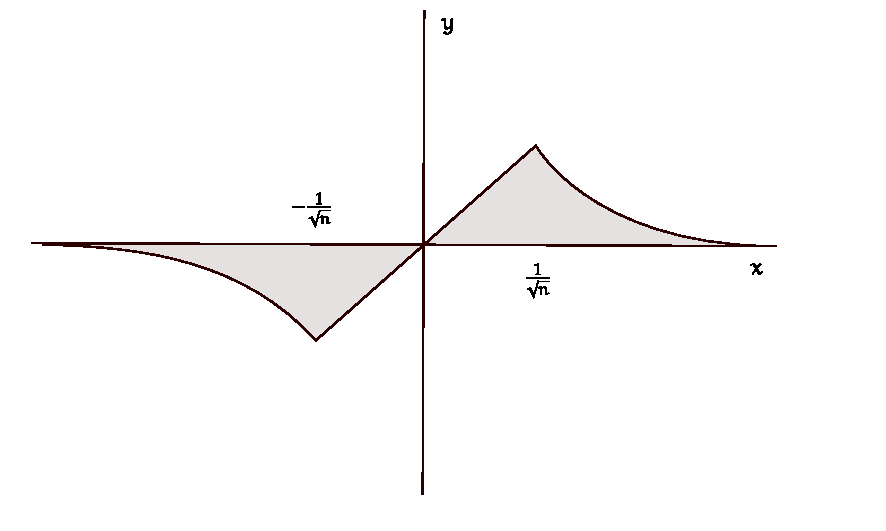
\includegraphics[scale = 0.9]{exmgraph1}
            \end{center}
        We have $\max(f_{n}(x)) = f_{n}(\frac{1}{\sqrt{n}}) = \frac{1}{2\sqrt{n}}$. And $\min(f_{n}(x)) = f_{n}(-\frac{1}{\sqrt{n}}) = \frac{-1}{2\sqrt{n}}$. So $\sup \{\lvert f_{n}(x) \rvert : s\in \mathbb{R}\} = \frac{1}{2\sqrt{n}} \rightarrow 0$. So $f_{n} \rightarrow 0$ uniformly converges.
    \end{example}
    \begin{example}
        Consider $f_{n}(x) = n^{2}x^{n}(1 - x)$. It converges when $x \in [0, 1]$. We have $\lim f_{n}(1) = 0$. If $0 \leq x< 1$, since $(n^{2}x^{n}(1 - x))^{\frac{1}{n}} = (n^{\frac{2}{n}})x(1 - x)^{\frac{1}{n}} \rightarrow x < 1$. So we know $\sum n^{2}x^{n}(1 - x)$ converges. Then $n^{2}x^{n}(1 - x) \rightarrow 0$. So $f_{n} \rightarrow 0$ pointwise. Check $ \sup \{\lvert f_{n}(x) \rvert : x \in [0, 1]\}$. Find the maximum and minimum values of $f_{n}$. Recall critical value theorem: If $f$ is differentiable on $[a, b]$, then maximum or minimum values are at one of the critical points $x$ such that $f^{\prime}(x) = 0$ or $a, b$. Find $f^{\prime}_{n}(x) = nx^{n - 1} - (n + 1)x^{n} = x^{n - 1}(n - (n + 1)x)$. So $f_{n}^{\prime}(x) = 0$. So $x = 0$ or $\frac{n}{n + 1}$. So $f_{n}(0) = f_{n}(1) = 0$. We have $f(\frac{n}{n + 1}) = \frac{n^{2}}{n + 1}(\frac{n}{n + 1})^{n}$. We consider what happens when $n \rightarrow \infty$. We have
            \begin{align*}
                (\dfrac{n}{n + 1})^{n} &=           \dfrac{1}{(\dfrac{n + 1}{n})^{n}} \\
                                       &=           \dfrac{1}{(1 + \dfrac{1}{n})^{n}} \\
                                       &=           \dfrac{1}{e}                      \\
                \dfrac{n^{2}}{n + 1}   &\rightarrow  \infty                             
            \end{align*}
         So $\frac{n^{2}}{n + 1}(\frac{n}{n + 1})^{n}$ goes to infinity, which is not $0$, so it is not uniformly convergent.
    \end{example} 
\end{examples}

\begin{theorem}{25.2}
    If $f_{n} \rightarrow f$ uniformly on $[a, b]$ and $f_{n}$ are continuous on $[a, b]$, then $\lim \int_{a}^{b} f_{n}(x) \, \dd{x}  = \int_{a}^{b} f(x) \, \dd{x} = \int_{a}^{b} \lim f_{n}(x) \, \dd{x}$
\end{theorem}

\textbf{Recall}:
    \begin{itemize}
        \item The integral $\int_{a}^{b} f(x) \, \dd{x} =$ signed area between $f(x)$ and $x$ coordinate on $[a, b]$
            \begin{center}
                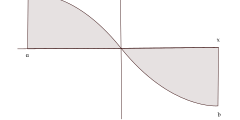
\includegraphics[scale = 0.9]{integralpic}
            \end{center}

        \item Any continuous function is integrable
        g(x)
        \item If $g(x) \leq h(x)$ $\forall x \in [a, b]$, then $\int_{a}^{b} g(x) \, \dd{x}  \leq \int_{a}^{b} h(x) \, \dd{x} $ 

        \item $\lvert \int_{a}^{b} g(x) \, \dd{x}  \rvert \leq \int_{a}^{b} \lvert g(x) \rvert  \, \dd{x}$
    \end{itemize}

\begin{proof}
    By theorem $24.3$, So $f$ is continuous. Then $f_{n} - f$ is integrable. Then $\forall \varepsilon> 0$, there is $N$ such that $\forall n> N$, $x \in [a, b]$, we have
        \begin{equation*}
            \lvert f_{n}(x) - f(x) \rvert < \dfrac{\varepsilon}{b - a}
        \end{equation*}
    Then $\forall n> N$, we have
        \begin{align*}
            \lvert \int_{a}^{b} f_{n}(x) \, \dd{x}  - \int_{a}^{b} f(x) \, \dd{x}  \rvert &= \lvert \int_{a}^{b} f_{n}(x) - f(x) \, \dd{x}  \rvert \\
                                                                                          &\leq \int_{a}^{b} \lvert f_{n}(x) - f(x) \rvert \, \dd{ x}  \\
                                                                                          &< \int_{a}^{b} \dfrac{\varepsilon}{ b - a} \, \dd{x}  \\
                                                                                          &= \varepsilon
        \end{align*}
    So $\lim \int_{a}^{b} f_{n}(x) \, \dd{x}  = \int_{a}^{b} f(x) \, \dd{x}$.
\end{proof}

\chapter{Week 11}

\textbf{Last Lecture}: $f_{n} \rightarrow f$ pointwise on $S$ if $\forall x \in S$, $\lim f_{n}(x) = f(x)$. Then $\forall  x\in S$, and $\forall \varepsilon> 0$, $\exists N$ such that $\forall n > N$, we have
    \begin{equation*}
        \lvert f_{n} (x) - f(x) \rvert < \varepsilon
    \end{equation*}
Definition: $f_{n} \rightarrow f$ uniformly if $\forall \varepsilon > 0$, $\exists N$ such that $\forall n > N$ and $x \in S$ we have
    \begin{equation*}
        \lvert f_{n}(x) - f(x) \rvert < \varepsilon
    \end{equation*}
Remark: $f_{n} \rightarrow f$ uniformly iff $\limsup \{\lvert f_{n}(x) - f(x) \rvert : x \in S\} = 0$. Theorem: If $f_{n} \rightarrow f$k uniformly on $[a, b]$ and $f_{n}$ is continuous, then 
    \begin{equation*}
        \lim \int_{a}^{b} f_{n}(x) \, \dd{x}  = \int_{a}^{b} f(x) \, \dd{x} 
    \end{equation*}
\begin{topic}
    \section{Series of Functions}
\end{topic}

\begin{definition}{Cauchy Series}
    $(f_{n})$ is uniformly cauchy on $S$ if $\forall \varepsilon> 0$, $\exists N$ such that $\forall x \in S$ and $m, n > N$, we have
        \begin{equation*}
            \lvert f_{n}(x) - f_{m}(x) \rvert < \varepsilon
        \end{equation*}
\end{definition}

\begin{theorem}{Uniform Convergence}
    If $(f_{n})$ uniformly cauchy on $S$, then $\exists f$ on $S$ such that $f_{n}\rightarrow f$ uniformly on $S$.
\end{theorem}

\begin{definition}{Series of Functions}
    $\sum_{k = 0}^{\infty} g_{k}$ is the limit if
        \begin{equation*}
            \sum_{k = 0}^{n}g_{k}
        \end{equation*}
    exist. If $\sum_{k = 0}^{n}g_{k}$ on uniformly on $S$, we say that the series is uniformly convergent.
\end{definition}

\begin{examples}
    \begin{example}
        Power Series: 
            \begin{equation*}
                \sum_{k = 0}^{\infty} a_{k}x^{k}
            \end{equation*}
        is a series of functions. $g_{k} = a_{k}x^{k}$.
    \end{example}
    \begin{example}
        $\sum_{k = 0}^{\infty}\frac{x^{n}}{1 + x^{n}}$ is a series of functions but not a power series.
    \end{example}
\end{examples}

\begin{definition}{Cauchy Criterion}
    The series converges uniformly on $S$ if $\forall \varepsilon > 0$, $\exists N$ such that $\forall n \geq m > N$ and $x \in S$, 
        \begin{equation*}
            \lvert \sum_{k = m}^{n}g_{k}(x) \rvert < \varepsilon
        \end{equation*}
\end{definition}

\begin{theorem}{25.6}
    If $\sum_{k = 0}^{\infty} g_{k}$ satisfies Cauchy criterion uniformly on $S$, then $\sum g_{k}$ converges uniformly on $S$.
\end{theorem}

\begin{theorem}{25.7}
    If real numbers $M_{k} \geq 0$ and $\sum M_{k} < \infty$, if $\lvert g_{k}(x) \rvert \leq M_{k}$ for any $x \in S$, then $\sum g_{k}$ converges uniformly on $S$. 
\end{theorem}
    \begin{proof}
        Prove Cauchy criterion uniformly on $S$. $\forall \varepsilon> 0$, $\sum M_{k}$ converges. So $\exists N$ such that $\forall n \geq m > N$ we have
            \begin{equation*}
                \sum_{k = m}^{n}M_{k} < \varepsilon
            \end{equation*}
        For any $x \in S$, $\lvert \sum_{k = m}^{n} g_{k}(x)\rvert \leq \sum_{k = m}^{n}\lvert g_{k}(x) \rvert \leq \sum_{k = m}^{n} M_{k} < \varepsilon$.
    \end{proof}

\begin{theorem}{25.5}
    If $g_{k}$ is continuous and $\sum_{k = 0}^{\infty}g_{k}$ converges uniformly on $S$, then the limit of the series is continuous.
\end{theorem}

\textbf{Remark}: If $\sum_{k = 0}^{\infty} g_{k}$ converges uniformly on $S$, then $(g_{k})$ converges to $0$ on $S$.

\begin{examples}
    \begin{example}
        Consider the power series $\sum_{k = 1}^{\infty} 2^{-k}x^{k}$. It converges pointwise to a continuous function on $(-2, 2)$ but not uniformly.
            \begin{proof}
                Take $a_{k} = 2^{-k}$, $\lim \sqrt[k]{a_{k}} = \frac{1}{2} = \beta$. Then $R = \frac{1}{\beta} = 2$. If $x = 2$, $\sum_{k = 1}^{\infty} 1$ diverges and if $x = -2$, $\sum_{-1}^{\infty} (-1)^{k}$ also diverges. Then radius of convergence is $(-2, 2)$. 

                (The limit is continuous on $(-2, 2)$). Take any $0 < a< 2$, then for any $x \in [-a, a]$, we have 
                    \begin{equation*}
                        \lvert 2^{-n}x^{n} \rvert \leq 2^{-n}a^{n} = \left(\dfrac{a}{2}\right)^{n}, \dfrac{a}{2} < 1
                    \end{equation*}
                so $\sum_{k = 0}^{\infty} g_{k}$ converges uniformly on $[-a, a]$. Then $\sum_{k = 1}^{\infty} 2^{-n}x^{n}$ is continuous on $[-a, a]$. Since $a$ is any number between $0, 2$, the limit is continuous on $(-2, 2)$.

                (Not uniform) Assume that the convergence is uniform. Then $(g_{k}) = x^{n}2^{-n}$ goes to $0$ uniformly on $(-2, 2)$. But $\sup \{\lvert x^{n}2^{-n} \rvert : x \in (-2, 2)\} = 1$. So contradiction.
            \end{proof}
    \end{example}
\end{examples}

\begin{theorem}{26.1}
    If we consider $\sum_{n = 0}^{\infty} a_{n}x^{n}$ which has radius of convergence $r > 0$, then the power series converges uniformly $[-R_{1}, R_{1}]$ where $0 <R_{1} < R$
\end{theorem}

\textbf{Corollary}: $\sum a_{n}x^{n}$ converges to a continuous function on $(-R, R)$. Remark: $\sum a_{n}x^{n}$ is not necessarily uniformly convergent on $(-R, R)$.

\begin{topic}
    \section{Derivative and Integral of Power Series}
\end{topic}

\textbf{Last Lecture}: Recall that $f_{n} \rightarrow f$ uniformly on $S$ if $\forall \varepsilon> 0$, $\exists N$ such that $\forall n > N$ and $x \in S$
    \begin{equation*}
        \lvert f_{n}(x) - f(x) \rvert < \varepsilon
    \end{equation*}
Theorem: If $(f_{n})$ are uniformly cauchy on $S$, then $\exists f$ such that $f_{n} \rightarrow f$ uniformly on $S$. 

Theorem for Series: If $\sum g_{k}$ satisfies the cauchy criterion on $S$, then $\sum g_{k}$ converges uniformly on $S$.

Theorem: If $M_{k} \geq 0$ and $\sum M_{k} < \infty$. If $\lvert g_{k}(x) \rvert \leq M_{k}$ $\forall x \in S$, $\forall k \in \mathbb{N}$, then $\sum g_{k}$ converges uniformly on $S$.

Theorem for power series: $\sum a_{n}x^{n}$ has $R> 0$. Then $\forall R_{1} < R$, the power series $\sum a_{n}x^{n}$ converges uniformly on $[-R_{1}, R_{1}]$.

Today: Derivative and integral on Power Series.

\textbf{Recall}: $(a_{n}x^{n})^{\prime} = na_{n}x^{n - 1}$ and $\int a_{n}x^{n} \, \dd{x}  = \frac{a_{n}}{a_{n + 1}}x^{n + 1}$. 

\textbf{Lemma}: If $\sum a_{n}x^{n}$ has $R$ then $\sum na_{n}x^{n}$ and $\sum\frac{a_{n}}{n + 1}x^{n + 1}$ have radius of convergence $R$.
    \begin{proof}
        We find $\beta = \limsup \lvert a_{n} \rvert^{\frac{1}{n}}, R = \frac{1}{\beta}$. Take $\limsup \lvert na_{n} \rvert^{\frac{1}{n}} = \limsup n^{\frac{1}{n}}\lvert a_{n} \rvert^{\frac{1}{n}} = \limsup \lvert a_{n} \rvert^{\frac{1}{n}} = \beta$. For the anti-derivative, we get:
            \begin{align*}
                \limsup \lvert \dfrac{a_{n}}{n + 1} \rvert^{\dfrac{1}{n}} &= \limsup \dfrac{\lvert a_{n} \rvert^{\dfrac{1}{n}}}{(n + 1)^{\dfrac{1}{n}}} \\
                                                                          &= \limsup \lvert a_{n} \rvert^{\dfrac{1}{n}} = \beta                           
            \end{align*}
    \end{proof}

\begin{theorem}{26.4}
    If $\sum a_{n}x^{n}$ has a radius $R > 0$, then $\forall \lvert x \rvert < R$, we have $\int_{0}^{x} \sum_{n = 0}^{\infty} a_{n}t^{n} \, \dd{t} = \sum_{n = 0}^{\infty}\frac{a_{n}}{n + 1}x^{n + 1}$.
\end{theorem}
    \begin{proof}
        If $x > 0$ and $\sum_{n = 0}^{\infty} a_{n}x^{n}$ and $\sum_{n = 0}^{\infty} \frac{a_{n + 1}}{n + 1}x^{n + 1}$ uniformly converge on $[0, x]$. Use the theorem by $25.2$ we have:
            \begin{align*}
                \int_{0}^{x} \sum_{n = 0}^{\infty} a_{n}t^{n} \, \dd{t} &= \int_{0}^{x} \lim\limits_{k \to \infty} \sum_{n = 0}^{k}a_{n}t^{n} \, \dd{t}  \\
                                                                        &= \lim\limits_{k \to \infty} \int_{0}^{x} \sum_{n = 0}^{k}a_{n}t^{n} \, \dd{t} \\
                                                                        &= \lim\limits_{k \to \infty} \sum_{n = 0}^{k}\int_{0}^{x} a_{n}t^{n} \, \dd{t} \\
                                                                        &= \lim\limits_{k \to  \infty} \sum_{n = 0}^{k} \dfrac{a_{n + 1}}{n + 1}x^{n + 1} \\
                                                                        &= \sum_{k = 0}^{\infty} \dfrac{a_{n + 1}}{n + 1}x^{n + 1}
            \end{align*}
    \end{proof}

\begin{theorem}{26.5}
    Assume that $f(x_{n}) = \sum_{n = 0}^{\infty} a_{n}x^{n}$ has $R> 0$. Then $f(x)$ is differentiable on $(-R, R)$ and $f^{\prime}(x) = \sum_{n = 0}^{\infty} na_{n}x^{n - 1}$.
\end{theorem}
    \begin{proof}
        Take $g(x) = \sum_{n = 0}^{\infty} na_{n}x^{n + 1}$. $\forall \lvert x \rvert < R$. Using the last theorem:
            \begin{align*}
                 \int_{0}^{x} f(t) \, \dd{t}  &= \sum_{n = 1}^{\infty} a_{n}x^{n} \\
                                              &= f(x) - a_{0}                       
            \end{align*}
        But
            \begin{equation*}
                f(x) =  \int_{0}^{x} g(t) \, \dd{t}  + a_{0}
            \end{equation*}
        and $g(t)$ is continuous on $(-R, R)$. By the fundamental theorem of calculus, $f^{\prime}(x) = g(x)$.
    \end{proof}

\begin{examples}
    \begin{example}
        Recall that $\sum_{n = 0}^{\infty} x^{n} = \frac{1}{1 - x}$ for $\lvert x \rvert < 1$. Then $R = 1$. So differentiate:
            \begin{equation*}
                \dfrac{1}{(1 - x)^{2}} = \sum_{n = 0}^{\infty} nx^{n - 1}
            \end{equation*}
        We can also integrate:
            \begin{equation*}
                -\ln(1 - x) = \sum_{n = 0}^{\infty}\dfrac{1}{n + 1}x^{n + 1}
            \end{equation*}
        for $\lvert x \rvert < 1$
    \end{example}
\end{examples}

\begin{theorem}{Abel's Theorem}
    If $f(x) = \sum_{n = 0}^{\infty} a_{n}x^{n}$ has $0 < R < \infty$, and if $f$ converges at $x = R$, then $f$ is continuous at $x = R$. If $f$ converges at $x = -R$, then $f$ is continuous at $x = -R$.
\end{theorem}

\begin{examples}
    \begin{example}
        $-\ln(1 - x) = \sum_{n = 0}^{\infty}\frac{x^{n + 1}}{n + 1}$ for $\lvert x \rvert < 1$. $\sum_{n = 0}^{\infty}\frac{x^{n + 1}}{n + 1}$ converges at $x = -1$. By Abel's theorem, it is continuous at $x = -1$. This means that $\forall x_{n} \rightarrow-1^{+}$, $\lim \frac{x_{n}^{n + 1}}{n + 1} = \frac{(-1)^{n + 1}}{n + 1} = -\ln(2)$. Then we get:
            \begin{equation*}
                \ln(2) = 1 - \dfrac{1}{2} + \dfrac{1}{3} - \dfrac{1}{4} + \cdots
            \end{equation*}
    \end{example}
\end{examples}

\chapter{Week 12}

\textbf{Last Lecture}: If $f(x) = \sum_{n = 0}^{\infty} a_{n}x^{n}$ has $R > 0$. Then $\forall \lvert x \rvert < R$,
    \begin{equation*}
        \int_{0}^{x} f(t) \, \dd{t}  = \sum_{n = 0}L^{\infty}\dfrac{a_{n}}{n + 1}x^{n + 1}
    \end{equation*}
and
    \begin{equation*}
        \dv{x}f(x) = \sum_{n = 1}^{\infty} na_{n}x^{n - 1}
    \end{equation*}

Abel's theorem: If $\sum a_{n}x^{n}$ has $\infty > R > 0$, if it converges at $R$ or $-R$, then it is continuous at $R$ or $-R$.

\begin{topic}
    \section{Derivatives}
\end{topic}

\begin{definition}{Derivative}
    Let $f$ be a function defined on an open interval containing $x_{0}$. Then $f$ is differentiable or $f$ has derivative at $x_{0}$ if $\lim\limits_{x \to x_{0}}\frac{f(x) - f(x_{0})}{x - x_{0}} = f^{\prime}(x_{0})$ converges.
\end{definition} 

\begin{examples}
    \begin{example}
        $g(x) = x^{2}$. We have $\lim\limits_{x \to x_{0}}\frac{g(x) - g(x_{0})}{x - x_{0}} = \lim\limits_{x \to x_{0}}\frac{x^{2} - x_{0}^{2}}{x - x_{0}}$:
            \begin{equation*}
                \lim\limits_{x \to x_{0}}\dfrac{(x - x_{0})(x + x_{0})}{x - x_{0}} = 2x_{0}
            \end{equation*}
        So $g^{\prime}(x) = 2x$. 
    \end{example}
\end{examples}

In general, $(x^{n})^{\prime} = nx^{n - 1}$.

\begin{theorem}{28.2}
    If $f$ is differentiable at $x_{0}$, then $f$ is continuous at $x_{0}$.
\end{theorem}
    \begin{proof}
        $\forall x \in \dom (f) - \{x_{0}\}$. Then $f(x) = (x - x_{0})\frac{f(x) - f(x_{0})}{x - x_{0}} + f(x_{0})$. If $x \rightarrow x_{0}$, $(x - x_{0}) \rightarrow 0$, $\frac{f(x)  f(x_{0})}{x - x_{0}} \rightarrow f^{\prime}(x_{0})$, and $f(x_{0}) \rightarrow f(x_{0})$. Therefore, $f(x) \rightarrow 0 \cdot f^{\prime}(x_{0}) + f(x_{0}) = f(x_{0})$. Then $f$ is continuous at $x_{0}$.
    \end{proof}

\begin{theorem}{28.3}
    If $f$ and $g$ are differentiable at $x_{0}$, then 
        \begin{itemize}
            \item $\forall c \in \mathbb{R}$, $(cf)^{\prime}(x_{0}) = ic \cdot f^{\prime}(x_{0})$.

            \item $(f + g)^{\prime}(x_{0}) = f^{\prime}(x_{0}) + g^{\prime}(x_{0})$

            \item $(fg)^{\prime}(x) = f^{\prime}(x_{0})g(x_{0}) + f(x_{0})g^{\prime}(x_{0})$ 

            \item If $g(x_{0}) \neq 0$, then $(\frac{f}{g})^{\prime}(x_{0}) = \frac{f^{\prime}(x_{0})g(x_{0}) - f(x_{0})g^{\prime}(x_{0})}{g^{2}(x_{0})}$
        \end{itemize}
\end{theorem}

\begin{proof}
    (III) Consider $\frac{(fg)(x) - (fg)(x_{0})}{x - x_{0}}$. We have:
        \begin{align*}
            \dfrac{f(x)g(x) - f(x)g(x_{0}) + f(x)g(x_{0}) - f(x_{0})g(x_{0})}{x - x_{0}} &=           f(x)\dfrac{g(x) - g(x_{0})}{x - x_{0}} + g(x_{0})\dfrac{f(x) - f(x_{0})}{x - x_{0}} \\
                                                                                         &\rightarrow  f(x_{0})g^{\prime}(x_{0}) + g(x_{0})g^{\prime}(x_{0})                                
        \end{align*}
    (IV) Consider $\frac{f}{g}(x) - \frac{f}{g}(x_{0})$
        \begin{align*}
            \dfrac{f(x)}{g(x)} - \dfrac{f(x_{0})}{g(x_{0})} &= \dfrac{f(x)g(x_{0}) - f(x_{0})g(x)}{g(x)g(x_{0})}                                       \\
                                                            &= \dfrac{f(x)g(x_{0}) - f(x_{0})g(x_{0}) + f(x_{0})g(x_{0}) - f(x_{0})g(x)}{g(x)g(x_{0})}   
        \end{align*}
    Then 
        \begin{equation*}
            \dfrac{\dfrac{f}{g}(x) - \dfrac{f}{g}(x_{0})}{x - x_{0}} = \dfrac{1}{g(x)g(x_{0})} \left(\dfrac{f(x) - f(x_{0})}{x - x_{0}}g(x_{0}) - f(x_{0}) \dfrac{g(x) - g(x_{0})}{x - x_{0}}\right)
        \end{equation*}
    Take $x \rightarrow x_{0}$:
        \begin{equation*}
            \dfrac{1}{g^{2}(x_{0})}\left(f^{\prime}(x_{0})g(x_{0}) - f(x_{0})g^{\prime}(x_{0})\right) = \dfrac{g(x_{0})f^{\prime}(x_{0}) - f(x_{0})g^{\prime}(x_{0})}{g^{2}(x_{0})}
        \end{equation*}
\end{proof}

\begin{theorem}{Chain Rule}
    If $f$ is differentiable at $x_{0}$ and $g$ is differentiable at $f(x_{0})$, then $(g \circ f)^{\prime}(x_{0}) = g^{\prime}(f(x_{0}))f^{\prime}(x_{0})$.
\end{theorem}
    \begin{proof}
        Show $\forall$ sequence $x_{n} \rightarrow x_{0}$, 
            \begin{equation*}
                \lim\limits_{n  \to \infty} \dfrac{(g \circ f)(x_{n}) - (g \circ f)(x_{0})}{ x_{n} - x_{0}} = g^{\prime}(f(x_{0}))f^{\prime}(x_{0})
            \end{equation*}
        Consider two cases:
            \begin{itemize}
                \item Case 1: Assume that $\exists$ an open interval $J$ containing $x_{0}$ such that $\forall x \in J - \{x_{0}\}$, $f(x) \neq f(x_{0})$. So $f(x_{n}) \neq f(x_{0})$ when $n$ is large. Then
                    \begin{align*}
                        \dfrac{(g \circ f)(x_{n}) - (g \circ f)(x_{0n})}{x_{n} - x_{0}} &= \dfrac{g(f(x_{n}))  - g(f(x_{0}))}{f(x_{n}) - f(x_{0})}\left(\dfrac{f(x_{n}) - f(x_{0})}{x_{0} - x_{0}}\right) \\
                                                                                        &= g^{\prime}(f(x_{0}))f^{\prime}(x_{0})                                                                            
                    \end{align*}
                So when $n \rightarrow \infty$, it goes to $g^{\prime}(f(x_{0})) f^{\prime}(x_{0})$

                \item If the assumption in case $1$ fails, there $\exists z_{n} \rightarrow x_{0}$, $z_{n} \neq x_{0}$ and $f(z_{n}) = f(x_{0})$. Then $\lim\limits_{n \to \infty}\frac{f(z_{n}) - f(x_{0})}{z_{n} - x_{0}} = 0 = g^{\prime}(f(x_{0}))f^{\prime}(x_{0})$. We need to show $(g \circ f)$ is differentiable at $x_{0}$ and derivative is $0$. Since $g^{\prime}(f(x_{0}))$ exists, then 
                    \begin{equation*}
                        \dfrac{g(y) - g(f(x_{0}))}{y - f(x_{0})}
                    \end{equation*}
                is bounded for any $y$ near $f(x_{0})$. That is, $\exists$ an open interval $I$ containing $f(x_{0})$ such that $\forall y \in I - \{f(x_{0})\}$, we have:
                    \begin{equation*}
                        \left\lvert \dfrac{g(y) - g(f(x_{0}))}{y - f(x_{0})} \right\rvert  \leq c
                    \end{equation*}
                then we have 
                    \begin{equation*}
                        \left\lvert \dfrac{(g \circ f)(x_{n}) - (g \circ f)(x_{0})}{x_{n} - x_{0})} \right\rvert \leq c \cdot \left\lvert \dfrac{f(x_{n}) - f(x_{0})}{x_{n} - x_{0}} \right\rvert
                    \end{equation*}
                This is because if $f(x_{n}) \neq f(x_{n})$, then $LHS$ is $\frac{(g \circ f)(x_{n}) - (g \circ f)(x_{0})}{f(x_{n}) - f(x_{n})} \frac{f(x_{n}) - f(x_{0})}{x_{n} - x_{0}}$. If $f(x_{n}) = f(x_{0})$, then $0 \leq c \cdot \lvert \ldots \rvert$. Using this inequality, we know that as we take the limit, as $n \rightarrow \infty$, we have that the RHS is equal to $0$. So the LHS goes to $0$. So we have $g^{\prime}(f(x_{0}))f^{\prime}(x_{0}) = 0 = (g \circ f)^{\prime}(x_{0})$ as desired.
            \end{itemize}
    \end{proof}

\begin{topic}
    \section{Mean Value Theorem}
\end{topic}

Last Lecture: $f$ is differentiable at $a$ if the derivative:
    \begin{equation*}
        f(a) = \lim\limits_{x \to a}\dfrac{f(x) - f(a)}{x - a}
    \end{equation*}
converges.

If $f$ is differentiable at $a$, then it is continuous at $a$. If $f$, $g$ are differentiable on $\mathbb{R}$ and $c \in \mathbb{R}$, then 
    \begin{itemize}
        \item  $(f + g)^{\prime}(x) = f^{\prime} + g^{\prime}$

        \item  $(cf)^{\prime} = cf^{\prime}$

        \item  $(fg)^{\prime} = f^{\prime}g + fg^{\prime}$

        \item $(\frac{f}{g})^{\prime} = \frac{f^{\prime}g - g^{\prime}f}{g^{2}}$ when $g(x) \neq 0$

        \item $(g \circ f)^{\prime}(x) = g^{\prime}(f(x))f^{\prime}(x)$ 
    \end{itemize}   

\begin{theorem}{29.1}
    If $f$ is defined on an open interval containing $x_{0}$ and assumes its maximum and minimum at $x_{0}$ and is differentiable, then $f^{\prime}(x_{0}) = 0$.
\end{theorem}
    \begin{proof}
        Let $f$ be defined on the interval $(a, b)$, achieving a maximum at $x_{0}$. For $x < x_{0}$, we have
            \begin{equation*}
                \dfrac{f(x) - f(x_{0})}{x - x_{0}}
            \end{equation*}
        So $f(x) < f(x_{0}), f(x) - f(x_{0}) \leq 0$. So $x - x_{0} < 0$. Then $f^{\prime}(x_{0}) \geq 0$. 

        Now for $x > x_{0}$, consider again $\frac{f(x) - f(x_{0})}{x - x_{0}}$. We have $f(x) - f(x_{0}) \leq 0$ and $x - x_{0} > 0$. So $f^{\prime}(x_{0}) \leq 0$. Then $f^{\prime}(x_{0}) = 0$ putting the two together.
    \end{proof}

Recall that any continuous function on $[a, b]$ achieves its maximum and minimum on $[a, b]$.

\begin{theorem}{Rolle's Theorem}
    Let $f : [a, b] \rightarrow \mathbb{R}$ be continuous. Suppose that it is differentiable on $(a, b)$. Suppose that $f(a) = f(b)$. Then there is $x \in (a, b)$ where $f^{\prime}(x) = 0$.
\end{theorem}
    \begin{proof}
        So there is $x_{0}, y_{0} \in [a, b]$ such that $f(x_{0})$ is the minimum of $f$ and $f(y_{0})$ is the max of $f$ on $[a, b]$. Then we have cases:
            \begin{itemize}
                \item $x_{0}, y_{0}$ are endpoint of $[a, b]$. Then $f$ is constant since $f(a) = f(b)$. Then $f^{\prime}(x) = 0$ for all $x \in (a, b)$.

                \item Otherwise, one of $x_{0}, y_{0} \in (a, b)$ and apply the previous theorem. 
            \end{itemize}
    \end{proof}

\begin{theorem}{Mean Value Theorem}
    Let $f$ be continuous on $[a, b]$, and differentiable on $(a, b)$. Then there exists $x \in (a, b)$ such that $f^{\prime}(x) = \frac{f(b) - f(a)}{b - a}$.
\end{theorem}
    \begin{proof}
        Consider the line on $[a, b]$ going through $f(a), f(b)$. Define 
            \begin{equation*}
                L = \dfrac{f(b) - f(a)}{b - a}(x - a) + f(a)
            \end{equation*}
        Then consider $f - L$. Since $(f - L)(a) = (f - L)(b) = 0$, we know that there is some $x \in (a, b)$ such that $(f - L)^{\prime}(x) = 0$. Then $f^{\prime}(x) - L^{\prime}(x) = 0$. So $f^{\prime}(x) = L^{\prime}(x)$. We have $L^{\prime}(x) = \frac{f(b) - f(a)}{b - a}$.
    \end{proof}

\textbf{Corollary}: If $f : (a, b) \rightarrow \mathbb{R}$ is differentiable and $f^{\prime}(x) = 0$ for $x \in (a, b)$, then $f$ is the constant function.
    \begin{proof}
        Suppose that there is some $f(x_{0}) \neq f(y_{0})$ then by mean value theorem, we have that $f^{\prime}(z_{0}) = \frac{f(x_{0}) - f(y_{0})}{x_{0} - y_{0}}$ which is not $0$.
    \end{proof}

\textbf{Corollary}: If $f, g$ are two differentiable functions on $(a, b) \rightarrow \mathbb{R}$ and $f^{\prime} = g^{\prime}$ on $(a, b)$, then there is some constant $c$ such that $f(x) = g(x) + c$.

\begin{definition}{Increasing, Strictly Increasing, Decreasing, Strictly Decreasing}
    Suppose $f$ is defined on an interval $I$. We say that $f$ is strictly increasing if on the interval $I$, for all $x_{1} , x_{2} \in I$, $x_{1} < x_{2}$, then $f(x_{1})k < f(x_{2})$. Similar definitions for other kinds of increasing/decreasing.
\end{definition}

\textbf{Corollary}: If $f : (a, b) \rightarrow \mathbb{R}$ is differentiable, then 
    \begin{itemize}
        \item  $f$ is strictly increasing if $f^{\prime}(x) > 0$ for all $x \in (a, b)$

        \item  $f$ is strictly decreasing if $f^{\prime}(x) < 0$ for all $x \in (a, b)$

        \item $f$ is increasing if $f^{\prime}(x) \geq 0$ for all $x \in (a, b)$

        \item $f$ is decreasing if $f^{\prime}(x) \leq 0$ for all $x \in (a, b)$ 
    \end{itemize}
    \begin{proof}
        If $f$ is not strictly increasing, then $\exists x_{1} < x_{2}$ such that $f(x_{1}) \geq f(x_{2})$. Then by mean value theorem we have $f^{\prime}(x) = \frac{f(x_{2}) - f(x_{1})}{x_{2} - x_{1}} \leq 0$, which contradicts that $f^{\prime}> 0$.
    \end{proof}

\begin{theorem}{Intermediate Value Theorem for Derivatives}
    Let $f: (a, b) \rightarrow \mathbb{R}$ be differentiable. If $a < x_{1} < x_{2}< b$ and $c$ is some value between $f^{\prime}(x_{1}), f^{\prime}(x_{2})$, then there is some $x_{1} < x < x_{2}$ such that $f^{\prime}(x) = c$.
\end{theorem}
    \begin{proof}
        Consider $g(x) = f(x) - cx$. This is differentiable on $(a, b)$. We can write $g^{\prime}(x_{1}) < 0 < g^{\prime}(x_{2})$. Then $g$ must assume its minimum in $[x_{1}, x_{2}]$. New $x_{1}$, we have 
            \begin{equation*}
                0 > g^{\prime}(x_{1}) = \lim\limits_{x \to x^{-}_{1}}\dfrac{g(x) - g(x_{1})}{x - x_{1}}
            \end{equation*}
        Then $g(x) - g(x_{1}) < 0$. So $g(x) < g(x_{1})$.

        Near $x_{2}$, we have $g^{\prime}(x_{2}) > 0$. Then we have
            \begin{equation*}
                0 < g^{\prime}(x_{2}) = \lim\limits_{x \to x_{2}^{-}}\dfrac{g(x) - g(x_{2})}{x - x_{2}}
            \end{equation*}
        We have $x - x_{2} < 0$. So $g(x) - g(x_{2}) < 0$ and $g(x) < g(x_{2})$. So the minimum of $g$ is in $(x_{1}, x_{2})$. So $g$ achieves its minimum at $x_{0} \in (x_{1}, x_{2})$, we have $g^{\prime}(x) = 0 = f^{\prime}(x) - c$. So $f^{\prime}(x) = c$.
    \end{proof}

\begin{examples}
    \begin{example}
        Consider the function $f : \mathbb{R} \rightarrow \mathbb{R}$ where 
            \begin{equation*}
                x \mapsto 
                    \begin{cases}
                        x^{2}\sin{\dfrac{1}{x}} & \text{ if $x \neq 0$} \\
                        0                       & \text{ if $x = 0$}      
                    \end{cases}
            \end{equation*}
        $f$ is differentiable on $\mathbb{R}$ but $f^{\prime}$ is not continuous at $x = 0$.
    \end{example}
\end{examples}

\chapter{Week 13}

\textbf{Last Lecture}: If $f$ is differentiable at $x_{0}$ and gets max/min at $x_{0}$ then $f(x_{0}) = 0$. Mean Value Theorem: If $f$ is continuous on $[a, b]$ and differentiable on $(a, b)$ then there exists $x \in (a, b)$ such that $f^{\prime}(x) = \frac{f(b) - f(a)}{b - a}$. 

Intermediate Value Theorem for derivatives: If $f$ is differentiable on $(a, b)$ and  $a < x_{1} < x_{2} < b$ and $c$ is between $f^{\prime}(x_{1})$ and $f^{\prime}(x_{2})$, then there is an $x \in (x_{1}, x_{2})$ such that $f^{\prime}(x) = c$.

\begin{topic}
    \section{Derivative of Inverse Functions}
\end{topic}

\begin{theorem}{29.9}
    Let $f$ be one-to-one continuous on $I$, $J = f(I)$. If $f$ is differentiable at $x_{0} \in I$, $f^{\prime}(x_{0}) \neq 0$, then $g = f^{-1}$ is differentiable at $f(x_{0}) = y$, $g^{\prime}(y_{0}) = \frac{1}{f^{\prime}(x_{0})}$.
\end{theorem}
    \begin{proof}
        $f(x) = y$, $g(y) = x$. Since $f$ is continuous and $I$ is connected, $J = f(I)$ is connected. So $J$ is an interval. $g : J \rightarrow I$, $F : I \rightarrow J$. So
            \begin{equation*}
                \lim\limits_{x \to x_{0}} \dfrac{f(x) - f(x_{0})}{x - x_{0}} = f^{\prime}(x_{0}) \neq 0
            \end{equation*}
        Then 
            \begin{align*}
                \lim\limits_{x \to x_{0}}\dfrac{x - x_{0}}{f(x) - f(x_{0})} &= \dfrac{1}{f^{\prime}(x_{0})} \neq 0                                                        \\
                                                                            &= \lim\limits_{x \to x_{0}}\dfrac{g(y) - g(y_{0})}{y - y_{0}} = \dfrac{1}{f^{\prime}(x_{0})}   
            \end{align*}
        We want to show that $\lim\limits_{y \to y_{0}} \iff \lim\limits_{x \to x_{0}}$. We want to show that $f, g$ continuous. By definition, $f$ is continuous and one-to-one. This means that $f$ is strictly increasing or decreasing by theorem $18.6$. This means that $g = f^{-1}$ is continuous by theorem $18.4$.
    \end{proof} 

\begin{examples}
    \begin{example}
        $f(x) = x^{n}, x \in [0, \infty)$. Then $f^{-1}(y) = g(y) = y^{\frac{1}{n}}, x \in [0, \infty)$. So $f^{\prime}(x) = nx^{n - 1}$ and $g^{\prime}(y) = \frac{1}{f^{\prime}(x)} = \frac{1}{nx^{n - 1}} = \frac{1}{n(y^{\frac{1}{n}})^{n - 1}}$. So this is $\frac{1}{n}y^{\frac{1}{n} - 1}$.
    \end{example}
\end{examples}

\begin{theorem}{Generalized MVT}
    Let $f, g$ be continuous on $[a, b]$ and differentiable at $(a, b)$. Then there exists $x \in (a, b)$ such that $f(x) (g(b) - g(a)) = g(x) (f(b) - f(a))$.
\end{theorem}

\textbf{Remark}: If $g(x) = x$, it is MVT.
    \begin{proof}
        If $h(x) = f(x)(g(b) - g(a)) - g(x)(f(b) - f(a))$. Take
            \begin{align*}
                h(b) &= f(b)g(b) - f(b)g(a) - g(b)f(b) + g(b)f(a) \\
                h(a) &= g(b)f(a) - f(b)g(a) = h(b)                  
            \end{align*}
        By Rolle's theorem, $\exists x \in (a, b)$ such that $h^{\prime}(x) = 0$.
    \end{proof}

\begin{theorem}{L'Hopital's Rule}
    Let $s$ signify $a, a^{+}, a^{-}, -\infty , \infty$ where $a \in \mathbb{R}$ with $f, g$ differentiable. Then limit
        \begin{equation*}
            \lim\limits_{x \to s}\dfrac{f^{\prime}(x)}{g^{\prime}(x)} = L
        \end{equation*}
    exists. If $\lim\limits_{x \to s}f(x) = \lim\limits_{x \to s}g(x) = 0$ or if $\lim\limits_{x \to s}\lvert g(x) \rvert = \infty$, then   
        \begin{equation*}
            \lim\limits_{x \to s}\dfrac{f(x)}{g(x)} = L
        \end{equation*}
\end{theorem}
    \begin{proof}
        Prove the case $s = a^{+}$ and $L$ is finite, 
            \begin{equation*}
                \lim\limits_{x \to s}f(x) = \lim\limits_{x \to s}g(x) = 0
            \end{equation*}
        Since $\lim\limits_{x \to a^{+}}\frac{f^{\prime}(x)}{g^{\prime}(x)} = L$ exists. $g^{\prime}(x)$ cannot be $0$ near $a^{+}$. By IVT for derivative $g^{\prime}(x)$ is always $> 0$ or $< 0$ near $a^{+}$ for $x \in (a, b)$. Assume $g^{\prime}(x) < 0$ for all $x \in (a, b)$. Then $g$ is strictly decreasing on $(a, b)$. So it is one-to-one on $(a, b)$. At most one $x \in (a, b)$ such that $g(x) = 0$. By choosing $b$ smaller, we assume $g(x)$ never vanishes on $(a, b)$. Then $\forall \varepsilon> 0$, $\exists \delta> 0$ such that $a + \delta < b$ and $\forall a < x < a + \delta$, we have 
            \begin{equation*}
                \lvert \dfrac{f^{\prime}(x)}{g^{\prime}(x)} - L \rvert < \varepsilon
            \end{equation*}
        So $\forall a  < y < x < a + \delta$, by theorem $30.1$, we have
            \begin{equation*}
                \dfrac{f(x) - f(y)}{g(x) - g(y)} = \dfrac{f^{\prime}(z)}{g^{\prime}(z)}
            \end{equation*}
        by generalized MVT for $z \in (x, y)$. So 
            \begin{equation*}
                \left\lvert \dfrac{f^{\prime}(z)}{g^{\prime}(z)} - L \right\rvert < \varepsilon
            \end{equation*}
        So
            \begin{align*}
                \left\lvert \dfrac{f(x) - f(y)}{g(x) - g(y)} - L \right\rvert &< \varepsilon   
            \end{align*} 
        Let $y \rightarrow a^{+}$. Then 
            \begin{equation*}
                \left\lvert \dfrac{f(x)}{g(x)} - L \right\rvert < \varepsilon
            \end{equation*}
        for $x \in (a, a+ \delta)$. So $\lim\limits_{x \to s}\frac{f(x)}{g(x)} = L$.
    \end{proof}

\begin{examples}
    \begin{example}
        Consider
            \begin{equation*}
                \lim\limits_{x \to 0}\dfrac{\sin{x}}{x}
            \end{equation*}
        The derivative of $\sin{x}$ is $\cos{x}$ and $\dv{x}x = 1$. We have
            \begin{equation*}
                \lim\limits_{x \to 0}\dfrac{\cos{x}}{1} = 1
            \end{equation*}
    \end{example}
    \begin{example}
        Consider
            \begin{equation*}
                \lim\limits_{x \to \infty}\dfrac{x^{2}}{e^{3x}}
            \end{equation*}
        We have $\dv{x}\frac{2x}{3e^{3x}}$, $\dv{x}\frac{2}{9e^{3x}} \rightarrow 0$. Then 
            \begin{equation*}
                \lim\limits_{x \to \infty}\dfrac{x^{2}}{e^{3x}} = 0
            \end{equation*}
    \end{example}
\end{examples}

\textbf{Last Lecture}: Let $f$ be one-to-one on $I$, $f$ is differentiable at $x_{0} \in I$, $f^{\prime}(x_{0}) \neq 0$ then $g = f^{-1}$ is differentiable at $y_{0} = f(x_{0})$, $g^{\prime}(y_{0}) = \frac{1}{f^{\prime}(x_{0})}$.

Let $S$ signify $a, a^{-}, a^{+}, \infty, -\infty$, $f, g$ differentiable. If 
    \begin{equation*}
        \lim\limits_{x \to s}\dfrac{f^{\prime}(x)}{g^{\prime}(x)} = L
    \end{equation*}
exists, if $\lim\limits_{x \to s}f(x) = \lim\limits_{x \to s}g(x) = 0$ or $\lim\limits_{x \to s} \lvert g(x) \rvert = \infty$, then $\lim\limits_{x \to s}\frac{f(x)}{g(x)} = L$.

\begin{examples}
    \begin{example}
        $\lim\limits_{x \to 0^{+}} x\ln{x}$. We can consider instead $x\ln{x} = \frac{\ln{x}}{\frac{1}{x}}$. Then the derivative is $\frac{\frac{1}{x}}{\frac{-1}{x^{2}}} = \lim\limits_{x \to 0^{+}}-x = 0$ 
    \end{example}
    \begin{example}
        $\lim\limits_{x \to 0^{+}}x^{x}$. Use $x = e^{\ln{x}}$. So
            \begin{align*}
                \lim\limits_{x \to  0^{+}}x^{x} &= \lim\limits_{x \to 0^{+}}(e^{\ln{x}})^{x} \\
                                                &= \lim\limits_{x \to 0^{+}}e^{x\ln{x}}      \\
                                                &= e^{0}                                     \\
                                                &= 1                                           
            \end{align*}
    \end{example}
    \begin{example}
        $\lim\limits_{x \to 0}h(x)$ where $h(x) = \frac{1}{e^{x} - 1} - \frac{1}{x}$. Then
            \begin{align*}
                h(x) &= \dfrac{x - e^{x} 1}{x(e^{x} - 1)}   
            \end{align*}
        Find the derivative:
            \begin{align*}
                \lim\limits_{x \to 0}\dfrac{1 - e^{x}}{e^{x} - 1 + xe^{x}} &\rightarrow  \lim\limits_{x \to 0}\dfrac{-e^{x}}{e^{x} + e^{x} + xe^{x}} \\
                                                                           &=           \dfrac{-1}{2}                                                  
            \end{align*}
    \end{example}
\end{examples}

Given $\sum_{k = 0}^{\infty} a_{k}x^{k}$ with $R > 0$. So $\sum_{k = 0}^{\infty} a_{k}x^{k} = f(x)$ on $(-R, R)$. It is differentiable. So we have $\sum_{k = 1}^{\infty} ka_{k}x^{k - 1} = f^{\prime}(x)$ on $(-R, R)$. We have
    \begin{equation*}
        f^{\prime}(0) = a_{1}
    \end{equation*}
Then $\sum_{k = 2}^{\infty} k(k - 1)a_{k}x^{k - 2} = f^{\prime\prime}(x)$. Then
    \begin{equation*}
        f^{\prime\prime}(0) = 2a_{2}
    \end{equation*}
Taking the derivative again: $\sum_{k = 3}^{\infty} k(k - 1)(k - 2)a_{k}x^{k - 3} = f^{\prime\prime\prime}(x)$. Then 
    \begin{equation*}
        f^{\prime\prime\prime}(0) = 6a_{3}
    \end{equation*}
If we continue, we get $f^{(n)}(0) = n! \cdot a_{n}$. Then $a_{k} = \frac{f^{(k)}(0)}{k!}$. Then
    \begin{equation*}
        f(x) = \sum_{k = 0}^{\infty}\dfrac{f^{(k)}(0)}{k!}x^{k}
    \end{equation*}
for $x \in (-R, R)$. We want to see if this equation is true for other functions like $\sin{x}, \cos{x}, \ldots$. 

\textbf{Remark}: Given $\sum_{k = 0}^{\infty} a_{k}(x - c)^{k}$, where $c$ is constant, with $c \in \mathbb{R}$, $R > 0$, we have
    \begin{equation*}
        f(x) = \sum_{k = 0}^{\infty}\dfrac{f^{(k)}(c)}{k!}(x - c)^{k}
    \end{equation*}
for $x \in (c - R, c + R)$.

\begin{definition}{Taylor Series}
    Let $f$ be a function defined on an open interval containing $c$, and $f$ has a derivative of all orders. Then we call $\sum_{k = 0}^{\infty}\frac{f^{(k)}(c)}{k!}(x - c)^{k}$ the Taylor Series. We call $R_{n}(x) = f(x) - \sum_{k = 0}^{n - 1}\frac{f^{(k)}(c)}{k!}(x - c)^{k}$ the remainder.
\end{definition}

\textbf{Remark}: $\sum_{k = 0}^{\infty}\frac{f^{(k)}(c)}{k!}(x - c)^{k}$ converges to $f(x)$ iff $\lim\limits_{n \to \infty}R_{n}(x) = 0$.

\begin{theorem}{31.3}
    Let $f$ be defined on $(a, b)$ such that $a < c < b$ and $f^{(n)}$ exists. Then $\forall x \neq c$ in $(a, b)$ $\exists y$ between $c$ and $x$ such that $R_{n}(x) = \frac{f^{(n)}(y)}{n!}(x - c)^{n}$.
\end{theorem}
    \begin{proof}
        Fix $x \neq c$ and $n \geq 1$. Let $M$ be the unique solution of the equation:
            \begin{equation*}
                f(x) = \sum_{k = 0}^{\infty} \dfrac{f^{(k)}(c)}{k!}(x - c)^{k} + M\dfrac{(x - c)^{n}}{n!}
            \end{equation*}
        We need to show that $f^{(n)}(y) = M$ for some $y$ between $x, c$. Let $g(t) = \sum_{k = 0}^{n - 1}\frac{f^{(k)}(0)}{k!}(t - c)^{k} + \frac{M(t - c)^{n}}{n!} - f(t)$. Then
            \begin{equation*}
                g(c) = f(c) - f(c) = 0
            \end{equation*}
        Consider $g^{\prime}(c) = f^{\prime}(c) - f^{\prime}(c) = 0$. So $g^{(k)}(c) = 0$ for $k < n$. Then $g(x) = 0$. By Rolle's Theorem, $\exists x_{1}$ between, $x, c$ such that $g^{\prime}(x_{1}) = 0$. By Rolle's Theorem for $g^{\prime}$, there exists $x_{2}$ between $x_{1}$, $c$ such that $g^{\prime\prime}(x_{2}) = 0$, and so on. Then there is $x_{n}$ such that $g^{(n)}(x_{n}) = 0$ for $x_{n}$ between $x_{n - 1}$ and $c$. Take $y = x_{n}$. Then $g^{(n)}(y) = 0$. So 
            \begin{equation*}
                g^{(n)}(y) = M - f^{(n)}(y) = 0
            \end{equation*}
    \end{proof}

\textbf{Corollary}: If $\lvert f^{(n)}(x) \rvert \leq c$, then $R_{n}(x) \rightarrow 0$.
    \begin{proof}
        We have $R_{n}(x) = \frac{f^{(n)}(y)}{n!}(x - c)^{n}$. Then it is $\leq \frac{c}{n!}(x - c)^{n} \rightarrow 0$.
    \end{proof}

\textbf{Last Lecture}: Recall that the Taylor Series for $f$ about $c$ is
    \begin{equation*}
        \sum_{k = 0}^{\infty}\dfrac{f^{(k)}(c)}{k!}(x - c)^{k}
    \end{equation*}
Remainder is $R_{n}(x) = f(x) - \sum_{k = 0}^{n - 1}\frac{f^{(k)}(c)}{k!}(x - c)^{k}$. We have
    \begin{equation*}
        f(x) = \text{Taylor Series}
    \end{equation*}
iff $\lim\limits_{n \to \infty} R_{n}(x) \rightarrow 0$.

Theorem: $\forall x \neq c$ in $(a, b)$, $\exists y$ between $x, c$ such that 
    \begin{equation*}
        R_{n}(x) = \dfrac{f^{(n)}(y)}{k!}(x - c)^{n}
    \end{equation*}

Corollary: If $\exists c> 0$ such that $\forall n \in \mathbb{N}$, $\lvert f^{(n)} \rvert < c$, then $R_{n}(x) \rightarrow 0$. So if the $n$-th derivative is always bounded, then $f(x)$ is equal to the Taylor series.

\begin{examples}
    \begin{example}
        Consider $f(x) = e^{x}$. We have $f^{(n)} = e^{x}$. We have $f^{(n)}(0) = 1$. So we want to show
            \begin{equation*}
                e^{x} = \sum_{k = 0}^{\infty}\dfrac{1}{k!}x^{k}
            \end{equation*}
        Then $\forall x \in \mathbb{R}$, $\exists M> 0$ such that $\lvert x \rvert< M$. On $(-M, M)$ $f^{(n)}$ is bounded by $e^{M}$.
    \end{example}
    \begin{example}
        $f(x) = \sin{x}$. We have
            \begin{equation*}
                f^{(n)}(x) = \begin{cases}
                    \cos{x} &\text{ if } n = 1 \\
                    -\sin{x} &\text{ if } n = 2 \\
                    -\cos{x} &\text{ if } n = 3 \\
                    \sin{}{x} &\text{ if } n = 4   
                \end{cases}
            \end{equation*}
        We have 
            \begin{equation*}
                f^{(n)}(0) = \begin{cases}
                    1 &\text{ if } n = 1, 4, 9, \ldots \\
                    -1 &\text{ if } n = 3, 7, 11, \ldots \\
                    0 &\text{ if } n = \text{ anything else }   
                \end{cases}
            \end{equation*}
        So for any odd number, $n = 2k + 1$. $f^{(n)}(0) = (-1)^{k}$. So the Taylor series is 
            \begin{equation*}
                \sum_{k = 0}^{\infty}\dfrac{(-1)^{k}}{(2k + 1)!}x^{2k + 1}
            \end{equation*}
        Since $\lvert f^{(n)}(x) \rvert \leq 1$, so by the corollary, 
            \begin{equation*}
                \sin{x} = \sum_{k = 0}^{\infty}\dfrac{(-1)^{k}}{(2k + 1)!}x^{2k + 1}
            \end{equation*}
    \end{example}
\end{examples}

\begin{theorem}{31.5}
    Let $f$ be defined on $(a, b)$ where $a < c < b$. If $f^{(n)}$ exists, and is continuous on $(a, b)$, then $\forall x \in (a, b)$, $R_{n}(x) = \int_{c}^{x} \frac{(x - t)^{n - 1}}{(n - 1)!}f^{(n)}(t) \, \dd{t} $.
\end{theorem}
    \begin{proof}
        For $n = 1$, only need to show that $R_{1}(x)  \int_{c}^{x} f^{\prime}(t) \, \dd{t} $. By definition, $R_{1}(x) = f(x)  - f(c) = \int_{c}^{x} f^{\prime}(t) \, \dd{t}$. In general, we will use induction on $n$ and integration by parts.
    \end{proof}

\textbf{Corollary}: $\forall x \neq c$ in $(a, b)$ there exists $y$ between $c$ and $x$ such that $R_{n}(x) = (x - c)\frac{(x - y)^{n - 1}}{(n - 1)!}f^{(n)}(y)$. This is called the cauchy form of the remainder.
    \begin{proof}
        Use theorem $31.5$ and IVT for integrals ($33.9$) covered later.
    \end{proof}

\begin{theorem}{Binomial Series Theorem}
    $\forall \alpha \in \mathbb{R}$, $\lvert x \rvert < 1$, then 
        \begin{equation*}
            (1 + x)^{\alpha} = 1 + \sum_{k = 1}^{\infty} \dfrac{\alpha (\alpha - 1) \cdots (\alpha - k + 1)}{k!} x^{k}
        \end{equation*}
\end{theorem}

\begin{proof}
    Let $f(x) = (1 + x)^{\alpha}$. Then $f^{\prime}(x) = \alpha(1 + x)^{\alpha - 1}$.  And $f^{\prime}(0k = \alpha)$. Then $f^{\prime\prime}(x) = \alpha (\alpha - 1)(1 + x)^{\alpha - 2}$. So $f^{\prime\prime}(0) = \alpha (\alpha - 1)$.

    In the right hand side, it is the Taylor series of $f$ about $0$. Only need to show that $\lim\limits_{n \to \infty} R_{n}(x) = 0$ $\forall \lvert x \rvert < 1$. Let $a_{k} = \frac{\alpha (\alpha - 1) \cdots (\alpha - k + 1)}{k!}$. Consider the ratio test:
        \begin{equation*}
            \lim \left\lvert \dfrac{a_{k + 1}}{a_{k}} \right\rvert = \lim\limits_{k \to \infty} \left\lvert \dfrac{a - k}{k + 1} \right\rvert = 1
        \end{equation*}
    So $\beta = 1$, $R = \frac{1}{\beta} = 1$. Similarly, $\sum ka_{k}x^{k - 1}$ has radius convergence of $1$. So $\forall \lvert x \rvert < 1$, we have $\lim ka_{k}x^{k - 1} =  0$. By previous corollary, $R_{n}(x) = (x - c)\frac{(x - y_{n})^{n - 1}}{(n - 1)!}f^{(n)}(y_{n})$. This is equal to $(x - c)\frac{(x - y_{n})^{n - 1}}{(n - 1)!}\alpha (\alpha - 1)\cdots (\alpha - k + 1)(1 + y_{n}^{\alpha - 1})$. Keep simplifying:   
        \begin{align*}
            \ldots &= x\dfrac{(x - y_{n})^{n - 1}}{(1 + y_{n})^{n - 1}}(1 + y_{n})^{\alpha - 1}na_{n}   
        \end{align*}
    Let $y_{n} = z_{n}x$, $z_{n} \in (0, 1)$. So 
        \begin{equation*}
            \left\lvert \dfrac{x - y_{n}}{1 + y_{n}} \right\rvert = \left\lvert \dfrac{x - z_{n}x}{1 + z_{n}x} \right\rvert = \lvert x \rvert\left\lvert \dfrac{1 - z_{n}}{1 + z_{n}}x \right\rvert < \lvert x \rvert
        \end{equation*}
    So
        \begin{align*}
            \lvert R_{n}(x) \rvert &= x\dfrac{(x - y_{n})^{n - 1}}{(1 + y_{n})^{n - 1}}(1 + y_{n})^{\alpha - 1}na_{n}  \\
                                   &< \lvert x \rvert \lvert x \rvert^{n - 1}na_{n}(1 + y_{n}^{\alpha - 1})
        \end{align*}
    Since $(1 + y_{n})^{\alpha - 1}$ is bounded and the other stuff converges to $0$, $\lvert R_{n}(x) \rvert \rightarrow 0$.
\end{proof}

\begin{examples}
    \begin{example}
        $f(x) \neq $ Taylor Series. Define
            \begin{equation*}
                f(x) = \begin{cases}
                    e^{\dfrac{-1}{x}} &\text{ if } x> 0 \\
                    0 &\text{ if } x \leq 0            
                \end{cases}
            \end{equation*}.
        Claim: $\forall n \in \mathbb{N}$, $f^{(n)}(0) = 0$. Taylor Series $= 0$. 

        We have 
            \begin{align*}
                \lim\limits_{x \to 0^{+}}\dfrac{f(x) - f(0)}{x - 0} &= \lim\limits_{x \to 0^{+}}\dfrac{e^{\dfrac{-1}{x}}}{x} \\
                                                                    &= \lim\limits_{x \to 0^{+}}\dfrac{\dfrac{1}{x}}{e^{\dfrac{1}{x}}}
            \end{align*}
        Use L'Hopital to get the limit is $0$. Then $\forall x > 0$, $f^{(n)}(x) = e^{\frac{-1}{x}} \cdot$ polynomial of $\frac{1}{x}$. We see that $f(x) \neq 0$ which is its Taylor Series.
    \end{example}
\end{examples}

\chapter{Week 14}

\textbf{Last Lecture}: Taylor Series:
    \begin{equation*}
        \sum_{k = 0}^{\infty} \dfrac{f^{(k)}(c)}{k!}(x - c)^{k}
    \end{equation*}
And
    \begin{equation*}
        R_{n}(x) = f(x) - \sum_{k = 0}^{n - 1}\dfrac{f^{k}(c)}{k!}(x -c)^{k}
    \end{equation*} 
Theorem: $R_{n}(x) = \int_{c}^{x} \frac{(x - c)^{n - 1}}{(n - 1)!}f^{(n)}(t) \, \dd{t} $. We had a corollary:
    \begin{equation*}
        R_{n}(x) = (x - c)\dfrac{(x - y)^{n - 1}}{(n - 1)!}f^{(n)}(y)
    \end{equation*}
And that $\forall \alpha \in \mathbb{R}, \lvert x \rvert < 1$ we have
    \begin{equation*}
        (1 + x)^{\alpha} = 1 + \sum_{k = 1}^{\infty}\dfrac{\alpha (\alpha - 1)\cdots (\alpha - k + 1)}{k!}x^{ k}
    \end{equation*}
\begin{topic}
    \section{Riemann Integral}
\end{topic}

\textbf{Idea}: If $f$ is a continuous function on $[a, b]$ then $\int_{a}^{b} f(x) \, \dd{x} $ is the area. We use rectangles to estimate.

\begin{definition}{Darboux Integral}
    Let $f$ be bounded on $[a, b]$. Then $\forall S \subseteq [a, b]$, define $M(f, S) = \sup \{f(x) : x \in S\}$. Define $m(f, S) = \inf \{f(x) : x \in S\}$. A partition of $[a, b]$ is 
        \begin{equation*}
            P = \{a = t_{0} < t_{1} < t_{2} < \cdots < t_{n} = b\}
        \end{equation*}
    The upper Darboux sum is 
        \begin{equation*}
            U(f, p) = \sum_{k = 1}^{n} M(f, [t_{k - 1}, t_{k}])(t_{k} - t_{k - 1})
        \end{equation*}
    and the lower Darboux sum
        \begin{equation*}
            L(f, P) = \sum_{k = 1}^{n}m(f, [t_{k - 1}, t_{k}])(t_{k} - t_{k - 1})
        \end{equation*}
    Then the upper Darboux integral:
        \begin{equation*}
            U(f) = \inf \{U(f, P) : P \text{ is a partition of $[a, b]$}\}
        \end{equation*}
    The lower Darboux integral:
        \begin{equation*}
            L(f) = \sup \{L(f, P) : P \text{ is a partition of $[a, b]$}\}
        \end{equation*}
    We say that $f$ is integral on $[a, b]$ if $U(f) = L(f)$. We write this as $\int_{a}^{b} f(x) \, \dd{x} $
\end{definition}

\begin{examples}
    \begin{example}
        (Non-Integrable) Define
            \begin{equation*}
                f(x) = \begin{cases}
                    0                     &\text{ if } x \text{ is irrational } \\
                    1 &\text{ if } x \text{ is rational}   
                \end{cases}
            \end{equation*}
        on $[a, b]$. We have   
            \begin{equation*}
                U(f, P) = \sum_{k = 1}^{n}M(f, [t_{k - 1}, t_{k}])(t_{k} - t_{k - 1})
            \end{equation*}
        Since $\mathbb{Q}$ is dense in $\mathbb{R}$, we have 
            \begin{equation*}
                U(f, P) = \sum_{k = 1}^{n}(t_{k} - t_{k - 1}) = b - a
            \end{equation*}
        Now for 
            \begin{equation*}
                L(f, P) = \sum_{k = 1}^{n}m(f, [t_{k - 1}, t_{k}])(t_{k} - t_{k - 1})
            \end{equation*}
        is
            \begin{equation*}
                L(f, P) = \sum_{k = 1}^{n}0 = 0
            \end{equation*}
        But $U(f) \neq L(f)$.
    \end{example}
\end{examples}

\textbf{Lemma}: If $P, Q$ are partitions, and $P \subseteq Q$, then $L(f, P) \leq L(f, Q) \leq U(f, Q) \leq U(f, P)$.

\textbf{Lemma}: If $P, Q$ are partitions, then we have $L(f, P) \leq U(f, Q)$.
    \begin{proof}
        Take $P \cup Q$ as a partition of $[a, b]$. Then 
            \begin{equation*}
                L(f, P) \leq L(f, P \cup Q) \leq U(f, P \cup Q) \leq U(f, Q)
            \end{equation*}
    \end{proof}

\begin{theorem}{32.4}
    We have $L(f) \leq U(f)$ by the previous lemma.
\end{theorem}

\begin{theorem}{32.5}
    Assume that $f$ is bounded in $[a, b]$. Then $f$ is integrable iff $\forall \varepsilon > 0$, there exists a partition $P$ such that $U(f, P) - L(f, P) < \varepsilon$.
\end{theorem}
    \begin{proof}
        $(\leftarrow)$ Suppose that $U(f, P) < L(f, P) + \varepsilon$. Then 
            \begin{equation*}
                U(f) \leq U(f, P) < L(f, P) + \varepsilon \leq L(f) + \varepsilon
            \end{equation*}
        then 
            \begin{equation*}
                U(f) \leq L(f) \text{ and } L(f) \leq U(f)
            \end{equation*}
        so $U(f) = L(f)$.

        ($\rightarrow$) $\forall \varepsilon> 0$, $\exists P_{1}, P_{2}$ such that 
            \begin{equation*}
                L(f, P_{1}) > L(f) - \dfrac{\varepsilon}{ 2}
            \end{equation*}
        and similarly,
            \begin{equation*}
                U(f, P_{2}) < U(f) + \dfrac{\varepsilon}{ 2}
            \end{equation*}
        Take $P = P_{1} \cup P_{2}$. Then 
            \begin{equation*}
                U(f, P) - L(f, P) \leq U(f, P_{2}) - L(f, P_{1}) < U(f) - L(f) + \varepsilon = \varepsilon
            \end{equation*}
    \end{proof}

\begin{definition}{Mesh}
    The mesh of $P = \{a = t_{0} < t_{1} < \cdots < t_{n} = b\}$ is
        \begin{equation*}
            \mathop{mesh}(P) = \max(t_{k} - t_{k - 1} : k = 1, 2, \ldots, n)
        \end{equation*}
\end{definition}

\begin{theorem}{32.7}
    Assume $f$ is bounded on $[a, b]$. Then $f$ is integrable iff $\forall \varepsilon> 0$ there exists $\delta > 0$ such that for any partition such that 
        \begin{equation*}
            \mathop{mesh}(P) < \delta
        \end{equation*}
    we have
        \begin{equation*}
            U(f, P) - L(f, P) < \varepsilon
        \end{equation*}
\end{theorem} 

\chapter{Week 15}

\begin{topic}
    \section{Properties of Integrals}
\end{topic}

\textbf{Last Lecture}: A partition on $[a, b]$ with $p = \{a = t_{0} < t_{ 1} < \cdots < t_{ n} = b\}$. The Darboux sum:
    \begin{equation*}
        U(f, P) = \sum_{ k = 1}^{n}M(f, [t_{k - 1}, t_{k}]) (t_{k} - t_{k - 1})
    \end{equation*}
and the lower Darboux sum
    \begin{equation*}
        L(f, P) = \sum_{ k = 1}^{n}m(f, [t_{k - 1}, t_{k}]) (t_{k} - t_{k - 1})
    \end{equation*}
The upper Darboux integral:
    \begin{equation*}
        U(f) = \inf \{ U(f, p) : p \text{ is a partition}\}
    \end{equation*}
and the lower Darboux integral:
    \begin{equation*}
        L(f) = \sup \{ L(f, p) : p \text{ is a partition}\}
    \end{equation*}
$f$ is integrable on $[a, b]$ if $U(f) = L(f)$ and we use:
    \begin{equation*}
        \int_{a}^{b} f(x) \, \dd{x} 
    \end{equation*}
We had that $\mathop{mesh}(P) = \max(t_{k} - t_{k - 1} : k = 1, 2, \ldots, n)$. Theorem: $f$ is integrable iff $\forall \varepsilon>  0$, $\exists \delta>  0$ such that $\forall P$ with mesh $ < \delta$, we had
    \begin{equation*}
        U(f, P) - L(f, P) < \varepsilon
    \end{equation*}

\begin{definition}{Riemann Sum}
    The Riemann sum of $f$ with $P$ is the sum of the form
        \begin{equation*}
            S = \sum_{ k = 1}^{n}f(x_{k})(t_{k} - t_{k - 1})
        \end{equation*}
    where $x_{k} \in [ t_{k - 1}, t_{k}]$. This is not unique such as $\sup S = U( f, P)$ and $\inf S = L( f, P)$.
\end{definition}

$f$ is Riemann integrable if $\exists r \in  \mathbb{ R}$ such that $\forall \varepsilon>  0$, $\exists \delta >  0$ such that $\forall \mathop{ mesh}(P) < \delta$, any Riemann sum $S$ of $f$ with $P$ we have
    \begin{equation*}
        \lvert S - r \rvert <  \varepsilon
    \end{equation*}  
We call $r$ is the Riemann integral.

\begin{theorem}{32.9}
    Riemann Integrable iff integrable.
\end{theorem}

\begin{theorem}{33.1}
    Any monotonic function $f$ on the closed interval $[a, b]$ is integrable 
\end{theorem}
    \begin{proof}
        $f$ is increasing. Then $\forall x \in  [ a, b]$ we have $f(a) \leq f( x) \leq f( b)$. So $\forall \varepsilon>  0$ take $\delta = \frac{ \varepsilon}{ f(b) - f(a)}$. Then $\forall \mathop{ mesh}(P) < \delta$, we want to show that
            \begin{equation*}
                U(f, P) - L(f, P) = \sum_{ k = 1}^{n}(M(f, [t_{k - 1}, t_{k}]) - m(f, [t_{k - 1}, t_{k}]) )(t_{k} - t_{k - 1})
            \end{equation*}
        Using the fact that $f$ is increasing:
            \begin{align*}
                \sum_{k = 1}^{n} = (f(t_{k}) - f(t_{k - 1}))(t_{k} - t_{k - 1}) &< \sum_{ k = 1}^{n}(f(t_{k}) - f(t_{k - 1}))\delta \\
                                                                                &= ( f(b) - f(a))\delta = \varepsilon
            \end{align*}
    \end{proof}

\begin{theorem}{33.2}
    Any continuous function on $[a,b]$ is integrable.
\end{theorem}
    \begin{proof}
        We have that $f$ is uniformly continuous. So $\forall \varepsilon>  0$, $\exists \delta > 0$ such that $\forall x, y \in  [ a, b]$ and 
            \begin{equation*}
                \lvert x - y \rvert <   \delta
            \end{equation*}
        We have
            \begin{equation*}
                 \lvert f(x) - f(y) \rvert < \dfrac{ \varepsilon}{ b - a}
            \end{equation*}
        $\forall \mathop{mesh}(P) < \delta$, we have that since $f$ is continuous on $[t_{k - 1}, t_{k}]$, $f$ achieves its maximum and minimum on the closed interval. We have
            \begin{equation*}
                M(f, [t_{k - 1}, t_{k}]) - m(f, [t_{k - 1}, t_{k}]) < \dfrac{ \varepsilon}{ b - a}
            \end{equation*}
        Then consider:
            \begin{align*}
                U(f, P) - L(f, P) &< \sum_{ k = 1}^{n}\dfrac{\varepsilon}{ b - a} (t_{k} - t_{k - 1}) \\
                                  &= \dfrac{\varepsilon}{ b - a}(b - a) = \varepsilon
            \end{align*}
    \end{proof}

\begin{theorem}{33.3}
    Assume $f$, $g$ are integrable on $[a, b]$ and $c \in \mathbb{ R}$. Then 
        \begin{itemize}
            \item  $\int_{a}^{b} cf(x) \, \dd{x}  = c\int_{a}^{b} f(x) \, \dd{x} $

            \item  $\int_{a}^{b} f(x) + g(x) \, \dd{x}  = \int_{a}^{b} f(x) \, \dd{x}  + \int_{a}^{b} g(x) \, \dd{x} $. 
        \end{itemize}
\end{theorem}

\begin{theorem}{33.4}
    \begin{itemize}
        \item If $f, g$ are integrable on $[a, b]$ and $f(x) \geq g( x)$, then 
            \begin{equation*}
                \int_{a}^{b} f(x) \, \dd{x}  \geq \int_{ a}^{b} g(x) \, \dd{x} 
            \end{equation*}

        \item If $g$ is continuous and $\geq 0$ on $[a, b]$ and 
            \begin{equation*}
                \int_{a}^{b} g(x) \, \dd{x} = 0
            \end{equation*}
        then $g = 0$ on $[a, b]$.
    \end{itemize}
\end{theorem}
    \begin{proof}
        (Part I) Take $h = f - g \geq 0$ on $ [a, b]$. Therefore, for any partition $P$, $L(h, P) \geq 0$. So $L(h) \geq 0$. So by the previous theorem, $h$ is integrable. So
            \begin{equation*}
                \int_{a}^{b} h(x) \, \dd{x}  = L(h) \geq 0
            \end{equation*}
        and
            \begin{equation*}
                \int_{a}^{b} f(x) \, \dd{x} \geq \int_{ a}^{b} g(x) \, \dd{x} 
            \end{equation*}
        so we are done.

        (Part II) Suppose that $g(t) > 0$ for some $ t \in [ a, b]$. So $\forall \varepsilon = \frac{g(t)}{2}$, $\exists \delta$ such that $\forall x \in  [ a, b]$ an
            \begin{equation*}
                \lvert x - t \rvert <  \delta
            \end{equation*}  
        we have
            \begin{equation*}
                \lvert g(x) - g(t) \rvert <  \dfrac{ g(t)}{2}
            \end{equation*}
        Then $g(x) > \frac{ g(t)}{2}$. So $\exists ( c, d) \subseteq [ a, b]$ such that 
            \begin{equation*}
                g(x) >\dfrac{ g(t)}{2} \text{ on } (c, d)
            \end{equation*}
        So
            \begin{equation*}
                \int_{a}^{b} g(x) \, \dd{x} \geq \int_{c}^{d} g(x) \, \dd{x} > \int_{ c}^{d} \dfrac{g(t)}{2} \, \dd{t} = \dfrac{g(t)}{2}(d - c) > 0
            \end{equation*}
        which is a contradiction.
    \end{proof}

\textbf{Last Lecture}: Riemann sums
    \begin{equation*}
        S = \sum_{ k = 1}^{n}f(x_{k}(t_{k} - t_{k - 1}))
    \end{equation*} 
where $x_{k} \in [ t_{k - 1}, t_{k}]$. A function is Riemann integrable iff $f$ is integrable.

Any monotone function is integrable. Any continuous function is integrable. 

Integration is linear operation. If $f \geq g$, then integral of $f$ is greater than that of $g$.

\begin{theorem}{33.5}
    If $f$ is integrable on $[a, b]$ then $\lvert f \rvert$ is integrable and
        \begin{equation*}
            \lvert \int_{a}^{b} f(x) \, \dd{x}  \rvert   \leq  \int_{ a}^{b} \lvert f(x) \rvert  \, \dd{x} 
        \end{equation*}
\end{theorem}
    \begin{proof}
        (Part I) $\forall \varepsilon>  0$, $\exists \delta>  0$ such that $\forall \mathop{mesh}(P) < \delta$ we have
            \begin{equation*}
                U(f, P) - L(f, P) < \varepsilon
            \end{equation*}
        \textbf{Claim}: $M(\lvert f \rvert, S) - m(\lvert f \rvert, S) \leq M( f, S) - m(f, S)$. 

        If $f$ is greater than or equal to $0$, they are the same. If some part of $f$ is less than $0$, $m(\lvert f \rvert, S)$ is greater than $m(f, S)$, positive. So the LHS is less than RHS. 

        Therefore, 
            \begin{align*}
                U(\lvert f \rvert, P) - L(\lvert f \rvert, P) &= \sum_{ k = 1}^{n}(M(\lvert f \rvert, [ t_{k - 1}, t_{k}]) - m(\lvert f \rvert, [ t_{k - 1}, t_{k}]))(t_{k} - t_{k - 1}) \\
                                                            &\leq \sum_{ k = 1}^{n}(M(f, [t_{k - 1}, t_{k}]) - m(f, [t_{k - 1}, t_{rk}]))(t_{k} - t_{k - 1}) \\
                                                            &= U(f, P) - L(f, P) < \varepsilon
            \end{align*} 
        So $ \lvert f \rvert$ is integrable.

        (Part II) We have $-\lvert f \rvert \leq  f \leq  \lvert  f \rvert$. We have
            \begin{equation*}
                -\int_{a}^{b}  \lvert f(x) \rvert  \, \dd{x}  \leq \int_{ a}^{b} f(x) \, \dd{x}  \leq \int_{ a}^{b} \lvert f(x) \rvert \, \dd{ x} 
            \end{equation*}
        So
            \begin{equation*}
                \lvert \int_{a}^{b} \lvert f(x) \rvert \, \dd{ x}  \rvert \leq  \int_{ a}^{b} \lvert f(x) \rvert \, \dd{ x} 
            \end{equation*}
    \end{proof}

\begin{theorem}{33.6}
    If $f$ is integrable on $[a, c]$ and $[c, b]$, then $f$ is integrable on $[a, b]$. Also, $\int_{a}^{b} f(x) \, \dd{x}  = \int_{a}^{c} f(x)j \, \dd{x}  + \int_{c}^{b} f(x) \, \dd{x} $.
\end{theorem}

\begin{theorem}{32.5}
    A function is integrable iff $\forall \varepsilon>  0$, $\exists P$ such that 
        \begin{equation*}
            U(f, P) - L(f, P) < \varepsilon
        \end{equation*}
\end{theorem}
    \begin{proof}
        Since $f$ is integrable on $[a, c]$, $[c, b]$, there exists a $P_{1}$ on $[a, c]$ and $P_{2}$ on $[c, b]$ such that 
            \begin{align*}
                U_{a}^{c}(f, P_{1}) - L_{a}^{c}(f, P_{1}) &< \dfrac{\varepsilon}{ 2} \\
                U_{c}^{b}(f, P_{2}) - L_{c}^{b}(f, P_{2}) &< \dfrac{\varepsilon}{ 2}   
            \end{align*}
        Take $P = P_{1} \cup P_{ 2}$ on $[a, b]$ and $U_{a}^{b}(f, P) = U_{a}^{c}(f, P_{1}) ++ U_{c}^{b}(f, P_{2})$, $L_{a}^{b}(f, P) = L_{a}^{c}(f, P_{1}) + L_{c}^{b}(f, P_{2})$. By the previous constraints,
            \begin{equation*}
                U_{a}^{b}(f, P) - L_{a}^{b}(f, P) < \varepsilon
            \end{equation*}
        So $f$ is integrable on $[a, b]$. We have 
            \begin{align*}
                \int_{a}^{b} f(x) \, \dd{x} &\leq U_{ a}^{b}(f, P) = U_{a}^{c}(f, P_{1}) + U_{c}^{b}(f, P_{2}) \\
                                            &< L_{ a}^{c}(f, P_{1} + \dfrac{\varepsilon}{ 2}) + L_{c}^{b}(f, P_{2}) + \dfrac{\varepsilon}{ 2} \\
                                            &\leq \int_{ a}^{c} f(x)  \, \dd{x} + \int_{c}^{b} f(x) \, \dd{x} + \varepsilon 
            \end{align*}
        Take $\varepsilon$ arbitrarily small:
            \begin{equation*}
                \int_{a}^{b} f(x) \, \dd{x} \leq \int_{ a}^{c} f(x) \, \dd{x}  + \int_{c}^{b} f(x) \, \dd{x} 
            \end{equation*}
        We have
            \begin{align*}
                \int_{a}^{b} f(x) \, \dd{x}  &\geq  L_{z}^{b}(f, P) = L_{a}^{c}(f, P_{1}) + L_{c}^{b}(f, P_{2}) \\
                                             &>     U_{a}^{c}(f, P_{1}) - \dfrac{\varepsilon}{ 2}               \\
                                             &\geq  \int_{a}^{c} f(x) \, \dd{x} + \int_{c}^{b} f(x) \, \dd{x}  - \varepsilon   
            \end{align*}
        take $\varepsilon$ arbitrarily small:
            \begin{equation*}
                \int_{a}^{b} f(x) \, \dd{x}  \geq \int_{ a}^{c} f(x) \, \dd{x}  + \int_{c}^{b} f(x) \, \dd{x} 
            \end{equation*}
        so they are equal.
    \end{proof} 

\begin{definition}{33.7}
    $f$ on $[a, b]$ is piecewise monotonic if $\exists P = \{ a = t_{0} < t_{ 1} < \cdots < t_{ n} = b\}$ such that $f$ is monotonic on each $(t_{k - 1}, t_{k})$. $f$ is piecewise continuous if $\exists P$ such that $f$ is uniformly continuous on each $(t_{k - 1}, t_{k})$.
\end{definition}

\begin{theorem}{33.8}
    If $f$ is piecewise continuous on $[a, b]$ or it is bounded and piecewise monotonic on $[a, b]$ then $f$ is integrable on $[a, b]$.
\end{theorem}

\begin{theorem}{Intermediate Value Theorem of Integrals}
    If $f$ is continuous on $[a, b]$, then $\exists x \in  ( a, b)$ such that $f(x) = \frac{1}{b - a}\int_{a}^{b} f(x) \, \dd{x} $.
\end{theorem}
    \begin{proof}
        Let $M = \max(f(x), x \in [ a, b])$. Let $m = \min(f(x), x \in [ a, b])$. If $M = m$, then $f$ is constant. Then for any $x$, $f(x) = \frac{1}{b - a}\int_{a}^{b} f(x) \, \dd{x} $. If $M \neq m$, then $M \geq f \geq  m$. Take the integral:
            \begin{equation*}
                \int_{a}^{b} M \, \dd{x} \geq \int_{ a}^{b} f(x) \, \dd{x} \geq \int_{ a}^{b} f(x) \, \dd{x} 
            \end{equation*}
        and
            \begin{equation*}
                 M \geq\dfrac{ 1}{b - a}\int_{a}^{b} f(x) \, \dd{x}  \geq m
            \end{equation*}
        By IVT, there exists $x \in  (a,b)$ such that $f(x) = \frac{1}{b - a}\int_{a}^{b} f(x) \, \dd{x} $.
    \end{proof}

\textbf{Last Lecture}: We had that $f$ is integrable then $\lvert f \rvert$ is integrable and that
    \begin{equation*}
        \lvert \int_{a}^{b} f(x) \, \dd{x}  \rvert \leq  \int_{ a}^{b} \lvert  f(x) \rvert \, \dd{ x} 
    \end{equation*}
Also, if $f$ is integrable on $[a, c]$ and $[c, b]$, then $f$ is integrable on $[a, b]$ and that 
    \begin{equation*}
        \int_{a}^{b} f(x) \, \dd{x}  = \int_{a}^{c} f(x) \, \dd{x}  + \int_{c}^{b} f(x) \, \dd{x} 
    \end{equation*}
Suppose that $f$ is piecewise continuous or piecewise monotonic. Then $f$ is integrable.

Theorem $33.9$ was the IVT for integrals. If $f$ is continuous on $[a, b]$, there there is $x \in ( a, b)$ such that 
    \begin{equation*}
        f(x) = \dfrac{1}{b - a}\int_{a}^{b} f(x) \, \dd{x} 
    \end{equation*}

\begin{topic}
    \section{Fundamental Theorem of Calculus}
\end{topic}

\begin{theorem}{}
    If $g$ is continuous on $[a, b]$, differentiable on $(a, b)$ and $g^{\prime}$ integrable on $[a, b]$, then 
        \begin{equation*}
            \int_{a}^{b} g^{\prime}(x) \, \dd{x}  = g(b) - g(a)
        \end{equation*}
\end{theorem}
    \begin{proof}
        $\forall \varepsilon>  0$, there is a partition $\{a = t_{0} \leq t_{ 1} \leq \cdots \leq  t_{ n} = b\}$. This a partition such that
            \begin{equation*}
                U(g^{\prime}, P) - L(g^{\prime}, P) < \varepsilon
            \end{equation*}
        For each $[t_{k - 1}, t_{k}]$, by MVT, there exists $x_{k} \in ( t_{k - 1}, t_{k})$ such that 
            \begin{equation*}
                g^{\prime}(x_{k}) = \dfrac{g(t_{k} - g_{t_{k - 1}}}{t_{k} - t_{k - 1}}
            \end{equation*}
        We have 
            \begin{align*}
                g(b) - g(a) &= \sum_{ k = 1}^{n}(g(t_{k}) - g(t_{k - 1}))\\
                            &= \sum_{k = 1}^{n}g^{\prime}(x_{k})(t_{k} - t_{k - 1})
            \end{align*}
        So we have $U(g^{\prime}, P) \geq g( b) - g(a) \geq L( g^{\prime}, P)$. We also have $U(g^{\prime}, P) \geq \int_{ a}^{b} g^{\prime}(x) \, \dd{x}  \geq L( g^{\prime}, P)$. So 
            \begin{equation*}
                \lvert \int_{a}^{b} g^{\prime}(x) \, \dd{x}  - (g(b) - g(a)) \rvert <  \varepsilon
            \end{equation*}
        Let $\varepsilon \rightarrow  0$. We have $\int_{a}^{b} g^{\prime}(x) \, \dd{x}  = g(b) - g(a)$.
    \end{proof}

\begin{theorem}{Integration by Parts}
    If $U, V$ are continuous on $[a, b]$, differentiable on $(a, b)$ and $U, V$ are integrable on $[a, b]$. Then we have
        \begin{equation*}
            \int_{a}^{b} U^{\prime}V + \int_{a}^{b} UV^{\prime} = U(b)V(b) - U(a)V(a)
        \end{equation*}
\end{theorem}
    \begin{proof}
        Let $g = uv, g^{\prime} = uv + vu$. Then 
            \begin{equation*}
                \int_{a}^{b} g^{\prime}(x) \, \dd{x}  = g(b) - g(a) = u(b)v(b) - u(a)v(a)
            \end{equation*}
    \end{proof}

\begin{examples}
    \begin{example}
        Find $\int_{   0}^{\pi} x\cos{x} \, \dd{x} $. Let $u = x$, $v = \sin{x}$, $v^{\prime} = \cos{x}$. Then
            \begin{equation*}
                \int_{0}^{\pi}  uv^{\prime} = u(\pi) v(\pi) - u(0)v(0) - \int_{a}^{b} u^{\prime}v^{\prime} 
            \end{equation*}
        This is 
            \begin{equation*}
                -\int_{0}^{\pi}  \sin{x} \, \dd{x}  = -(-\cos{x}))\eval_{0}^{\pi} = \cos{\pi} - \cos{0} = -2
            \end{equation*}
    \end{example}
\end{examples}

\begin{theorem}{Fundamental Theorem of Calc II}
    If $f$ is integrable on $[a, b]$, let 
        \begin{equation*}
            F(x) = \int_{a}^{x} f(t) \, \dd{t} , \, \forall x \in  [ a, b]
        \end{equation*}
    Then $F$ is continuous. If $f$ is is continuous at $x_{0} \in ( a, b)$, then $F$ derivative at $x_{0}$: $F^{\prime}(x_{0}) = f(x_{0})$. 
\end{theorem}
    \begin{proof}
        Choose $B > 0$ such that $\lvert f \rvert \leq  B$. Then $\forall \varepsilon>  0$, let $\delta = \frac{ \varepsilon}{ B}$. Then $\forall x, y \in  [ a, b]$ and $\lvert x - y \rvert <  \delta$, we have 
            \begin{equation*}
                \lvert F(x) - F(y) \rvert = \lvert  \int_{a}^{x} f(t) \, \dd{t}  - \int_{a}^{y} f(t) \, \dd{t}  \rvert = \lvert  \int_{y}^{x} f(t) \, \dd{t}  \rvert
            \end{equation*}
        This is less than or equal to $\int_{y}^{x} \lvert f(t) \rvert \, \dd{ t}$, $x > y$. Since $\lvert f \rvert \leq  B$, we have 
            \begin{equation*}
                \int_{y}^{x} \lvert f(t) \rvert \, \dd{ t}  \leq \int_{ y}^{x} B \, \dd{t} =  ( x - y)B < \varepsilon
            \end{equation*}
        (Part II) Suppose that $f$ is continuous at $x_{0}$. Then $\forall \varepsilon>  0$, we have $\exists \delta > 0$ such that $\forall t\in  ( a, b)$, $\lvert t - x \rvert <   \delta$, we have
            \begin{equation*}
                \lvert f(t) - f(x_{0}) \rvert <  \varepsilon
            \end{equation*}
        So $\forall x \in  [ a, b]$ and $  \lvert x - x_{0} \rvert < \delta$. We have 
            \begin{align*}
                \left\lvert \dfrac{F(x) - F(x_{0})}{x - x_{0}} - f( x_{0}) \right\rvert &= \left\lvert \dfrac{1}{x - x_{0}}(\int_{a}^{x} f(t) \, \dd{t}  - \int_{a}^{x_{0}} f(t) \, \dd{t} ) - f(x_{0}) \right\rvert \\
                                                                                        &= \left\lvert \dfrac{1}{x - x_{0}}\int_{x_{0}}^{x} f(t) \, \dd{t} - \dfrac{1}{x - x_{0}}\int_{x_{0}}^{x} f(x_{0}) \, \dd{t}  \right\rvert \\
                                                                                        &= \left\lvert \dfrac{1}{x - x_{0}} \int_{x_{0}}^{x} f(t) - f(x_{0}) \, \dd{t}  \right\rvert \\
                                                                                        &\leq \dfrac{1}{x - x_{0}} \int_{x_{0}}^{x} \lvert f(t) - f(x_{0}) \rvert \, \dd{ t} \\
                                                                                        &< \dfrac{ 1}{x - x_{0}} \int_{x_{0}}^{x} \varepsilon \, \dd{ t}  \\
                                                                                        &= \varepsilon
            \end{align*}
         So $F^{\prime}(x_{0}) = f(x_{0})$.
    \end{proof}

\begin{theorem}{Change of Variables}
    If $u$ is differentiable on an open interval $J$ and $u(J) \subseteq I$, $f$ is continuous on $I$. Then $f \circ u$ is continuous on $I$. Also, 
        \begin{equation*}
            \int_{a}^{b} f \circ u(x)u^{\prime}(x) \, \dd{x}  = \int_{u(a)}^{u(b)} f(t) \, \dd{t} 
        \end{equation*}
    for $a, b \in J$.
\end{theorem}
    \begin{proof}
        Fix $c \in I$, let $ F(u) = \int_{c}^{a} f(t) \, \dd{t} $. Then $F^{\prime}(u) = f(u)$ for $u \in J$. Let $g = F \circ u$. Then $g^{\prime} = F^{\prime}(u(x))u^{\prime}(x)$. Then
            \begin{equation*}
                \int_{a}^{b} f(u(x))u^{\prime}(x) \, \dd{x} = \int_{a}^{b} g^{\prime}(x) \, \dd{x} 
            \end{equation*}
        and by the First fundamental theorem
            \begin{align*}
                \int_{a}^{b} g^{\prime}(x) \, \dd{x} &= g(b) - g(a) \\
                                                     &= F(u(b)) - F(u(a)) \\
                                                     &= \int_{u(a)}^{u(b)} f(t) \, \dd{t} 
            \end{align*}
    \end{proof}











\end{document}
